\appendix

\section{Motivation for reconstruction methods}
\label{sec:motivation_for_reconstruction_methods}

Figure~\ref{fig:appendix_reconstruction} shows a comparison of
performances of the outside-in and the inside-out (the one used in
this analysis) muon identification algorithms in Monte Carlo. The
plots show the probability of finding both muons in a simulation
sample of the dimuon events with a flat invariant mass
distribution. Efficiencies are shown as a function of the separation
of their trajectories in the muon system.

To quantify the separation of muon trajectories, we construct a
cylinder with 600~cm radius, centered on the beamline, and two planes
transverse to the beamline and 700~cm from the interaction point.  The
muon trajectories are propagated to the cylinder if $|\eta| < 1$
(barrel) and are propagated to one of the planes if $|\eta| > 1$
(endcaps).  The difference in azimuthal coordinate of the two muon
trajectories on these surfaces are called $\Delta \phi$.  Closeness in
the other coordinate is quantified by $\Delta z/r$ on the cylinder and
$\Delta r/z$ on the planes.  Figure~\ref{fig:appendix_reconstruction}
shows efficiency as a function of $\Delta \phi$ with a cut on $\Delta
z/r$ and $\Delta r/z$ for the barrel and endcaps, respectively.

The defficiencies of the outside-in reconstruction are due to
confusion of ``stand-alone'' segment-only track-finding in the muon
system when multiple muons are present.  One of the two muons is
almost always found (important for trigger efficiency), but not both
(important for offline reconstruction).  In the barrel, the shape of
the inefficient region in $\Delta \phi$ is complicated by muon energy
loss: the propagation of trajectory into the muon system was done on
the basis of generator-level parameters at the interaction point.
As the $p_T$ of the muons increases, the shape of the inefficient
region consolidates and symmetrizes around $\Delta \phi = 0$.

The inside-out reconstruction algorithm used by this analysis is much
less sensitive to overlapping muons.  Only a small dip can be seen in
the endcap, analyzed in more detail in Fig.~\ref{fig:recoefficiency}
in the main text.

\begin{figure}
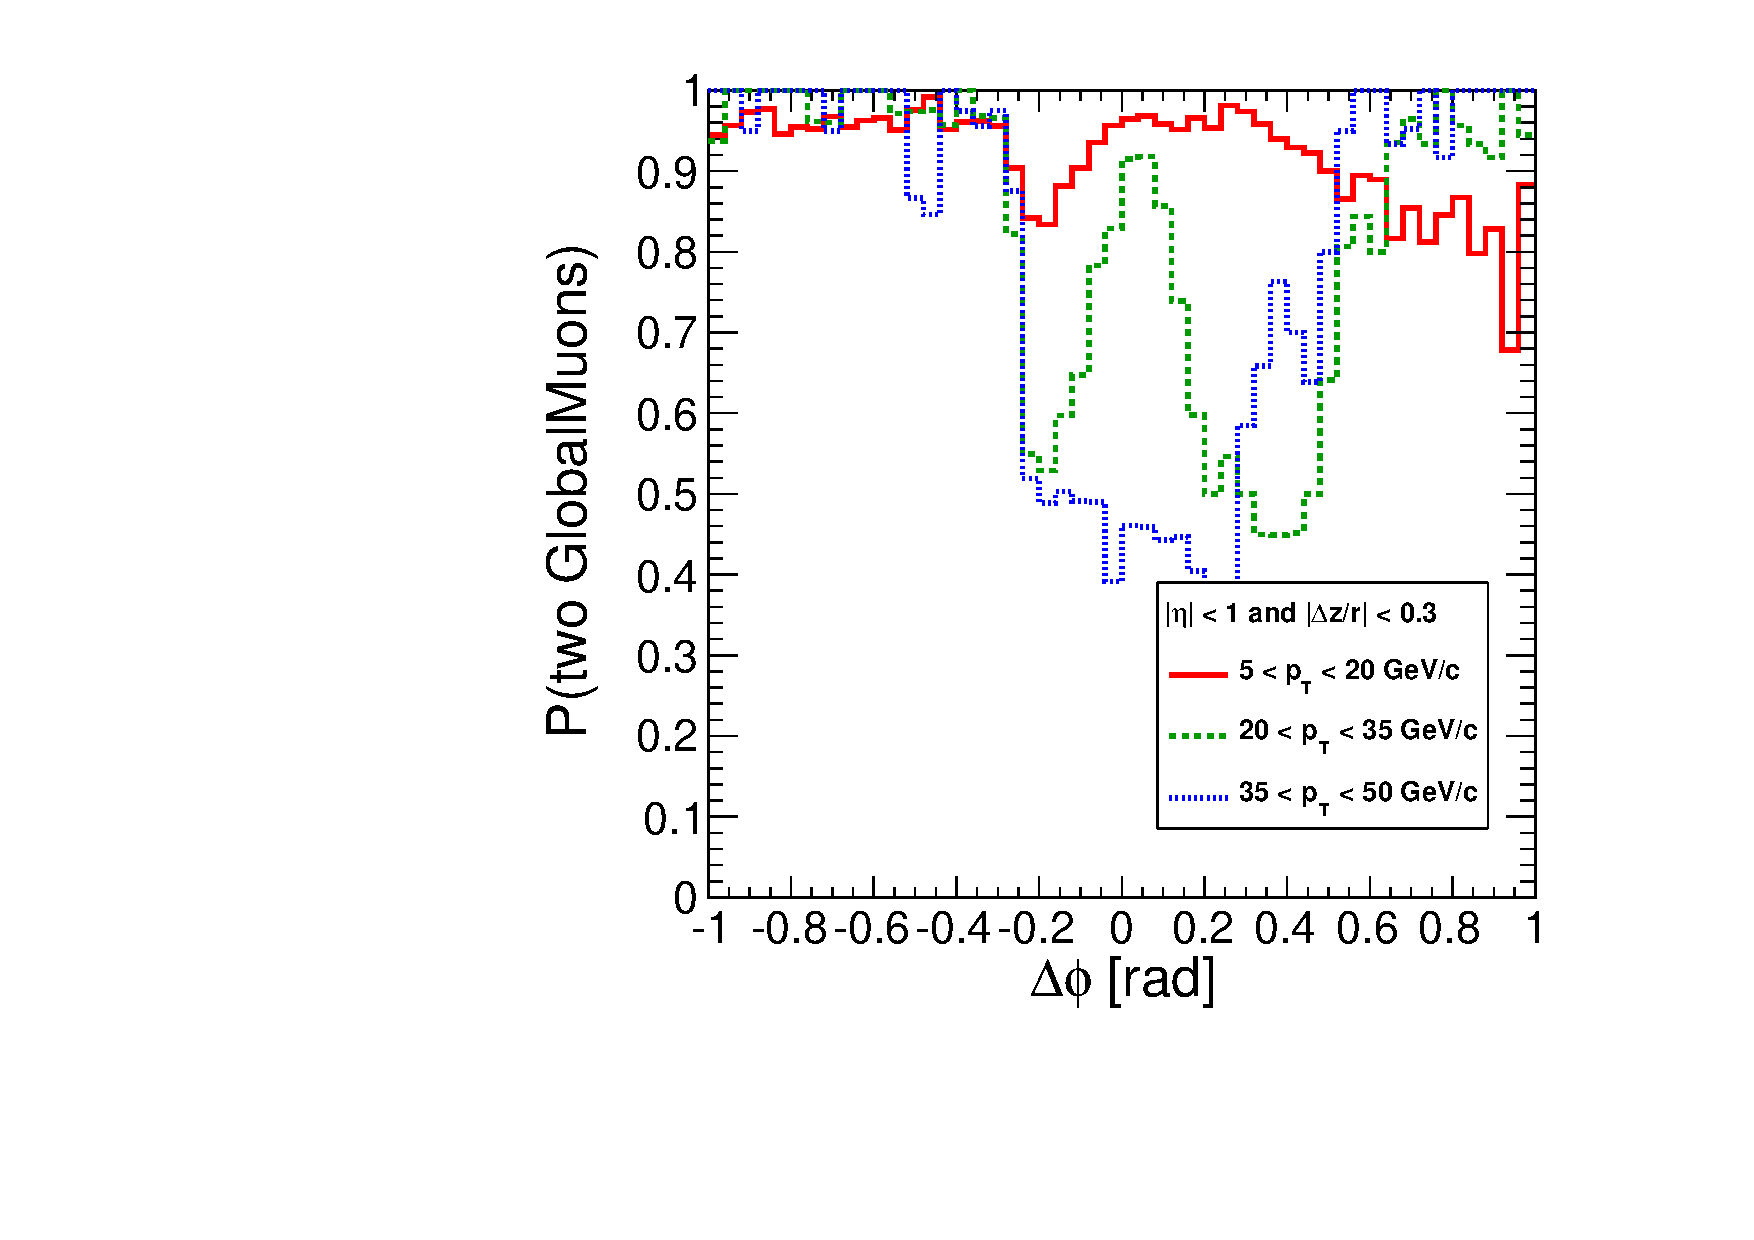
\includegraphics[width=0.48\linewidth]{PLOTS/barrel_dphi_bypt_twoGlobalMuons.pdf} \hfill
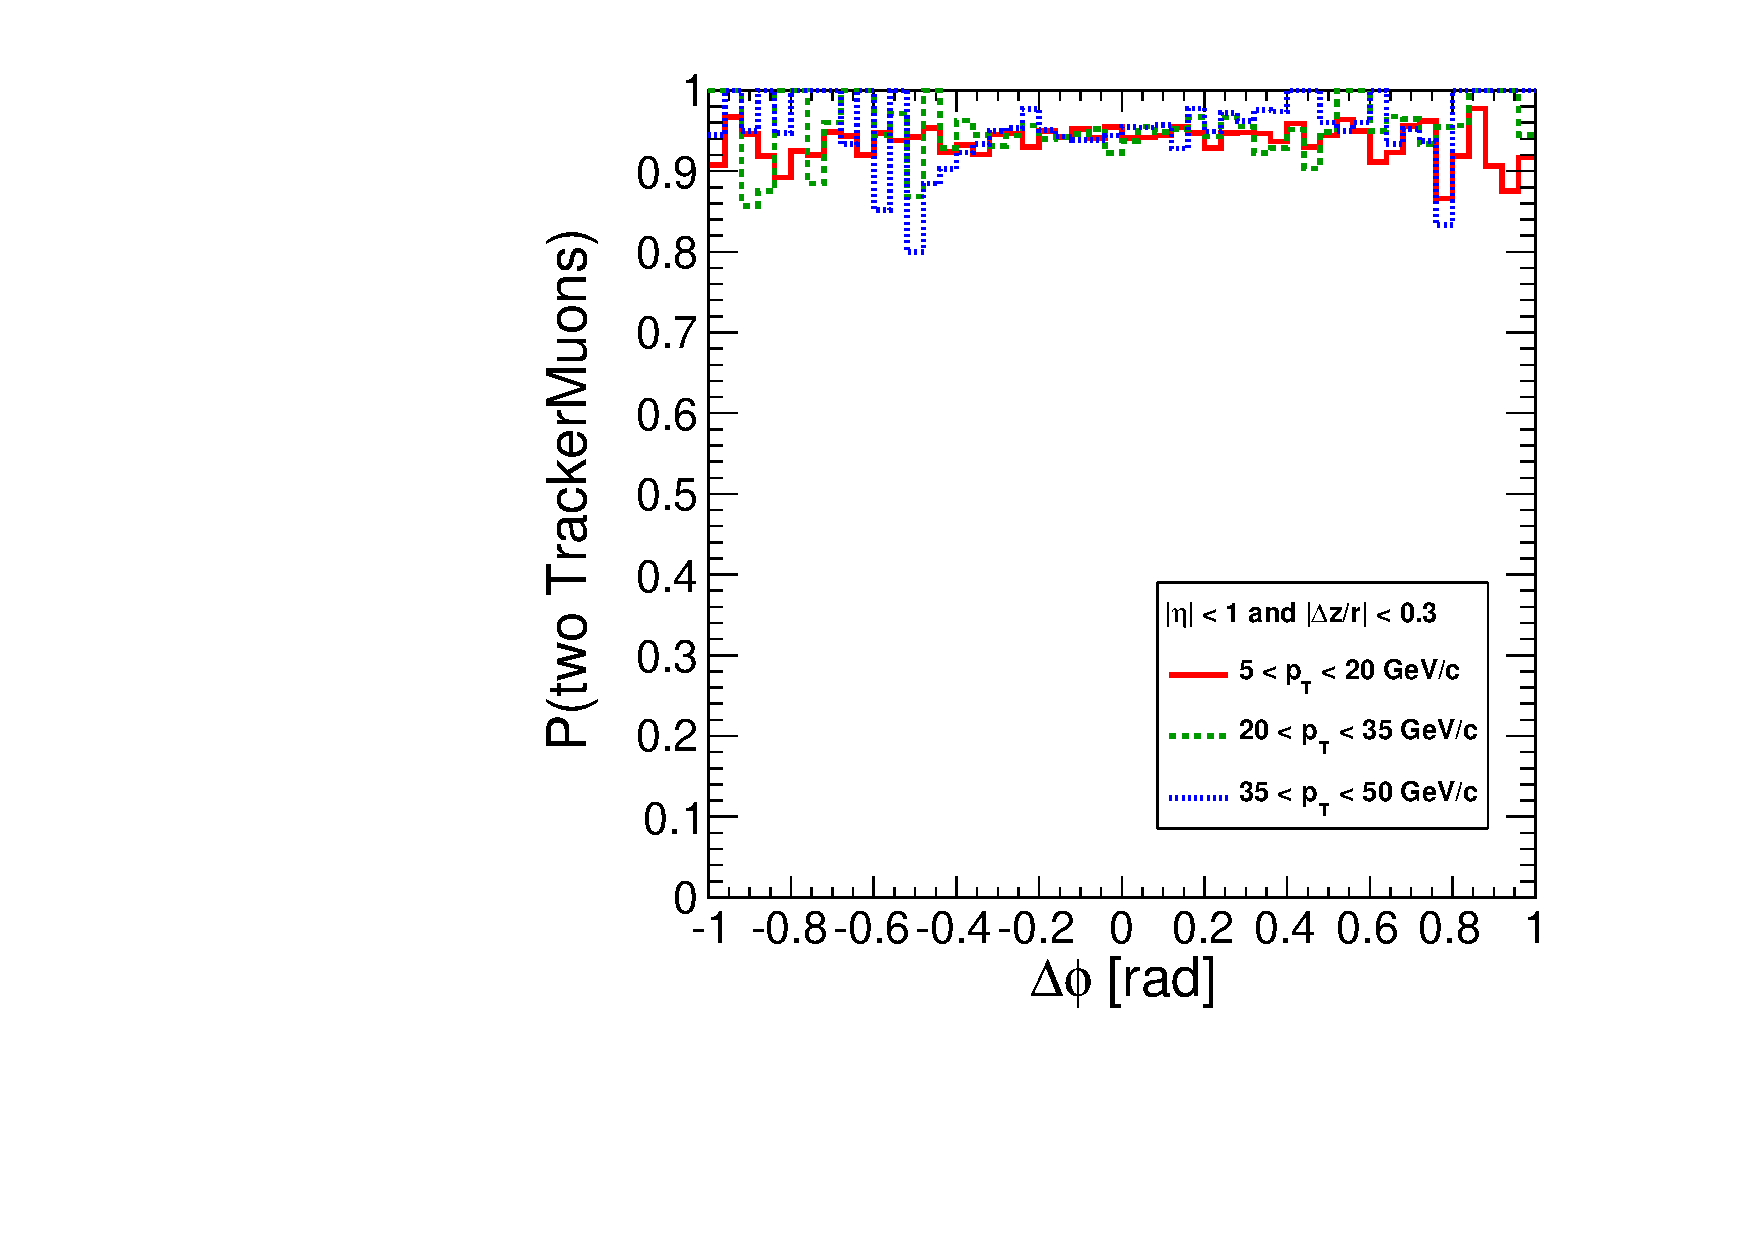
\includegraphics[width=0.48\linewidth]{PLOTS/barrel_dphi_bypt_twoTrackerMuons.pdf}
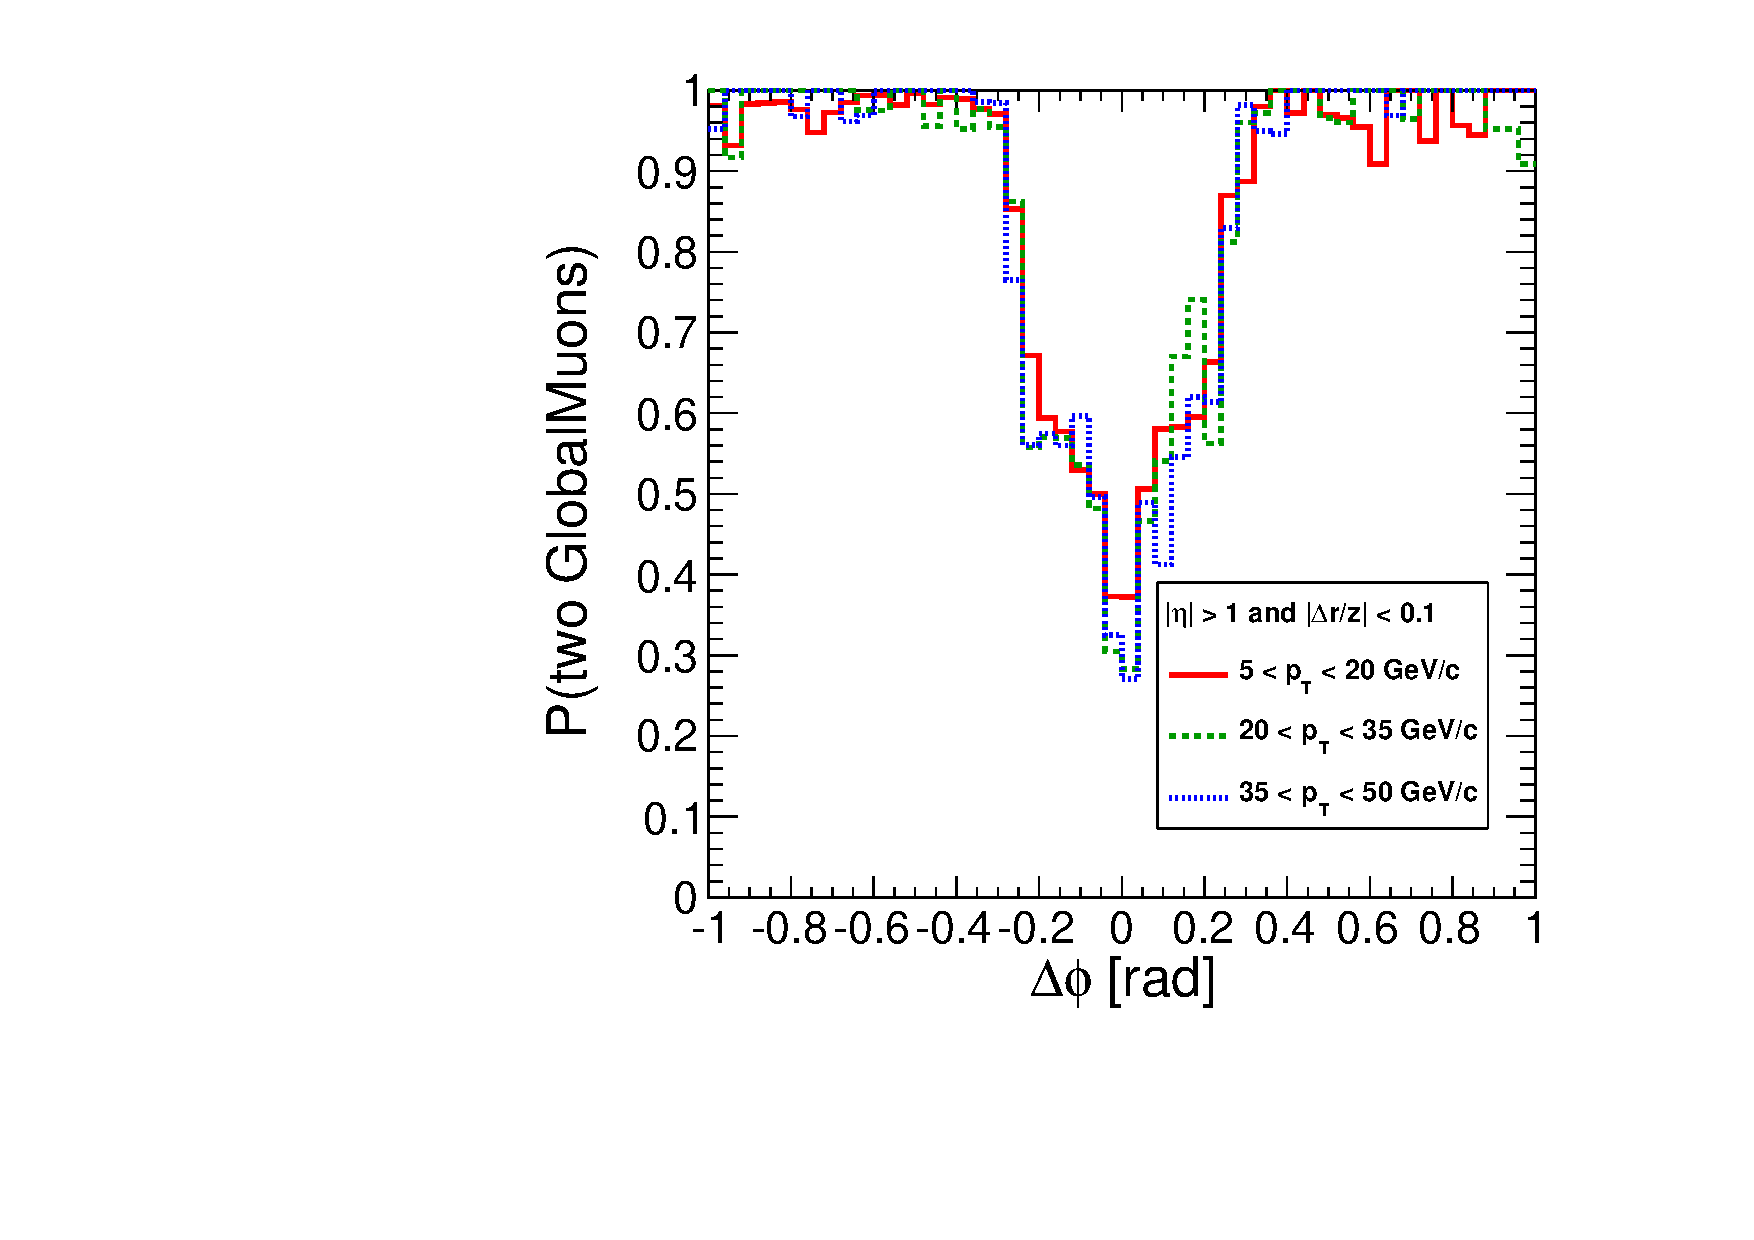
\includegraphics[width=0.48\linewidth]{PLOTS/endcap_dphi_bypt_twoGlobalMuons.pdf} \hfill
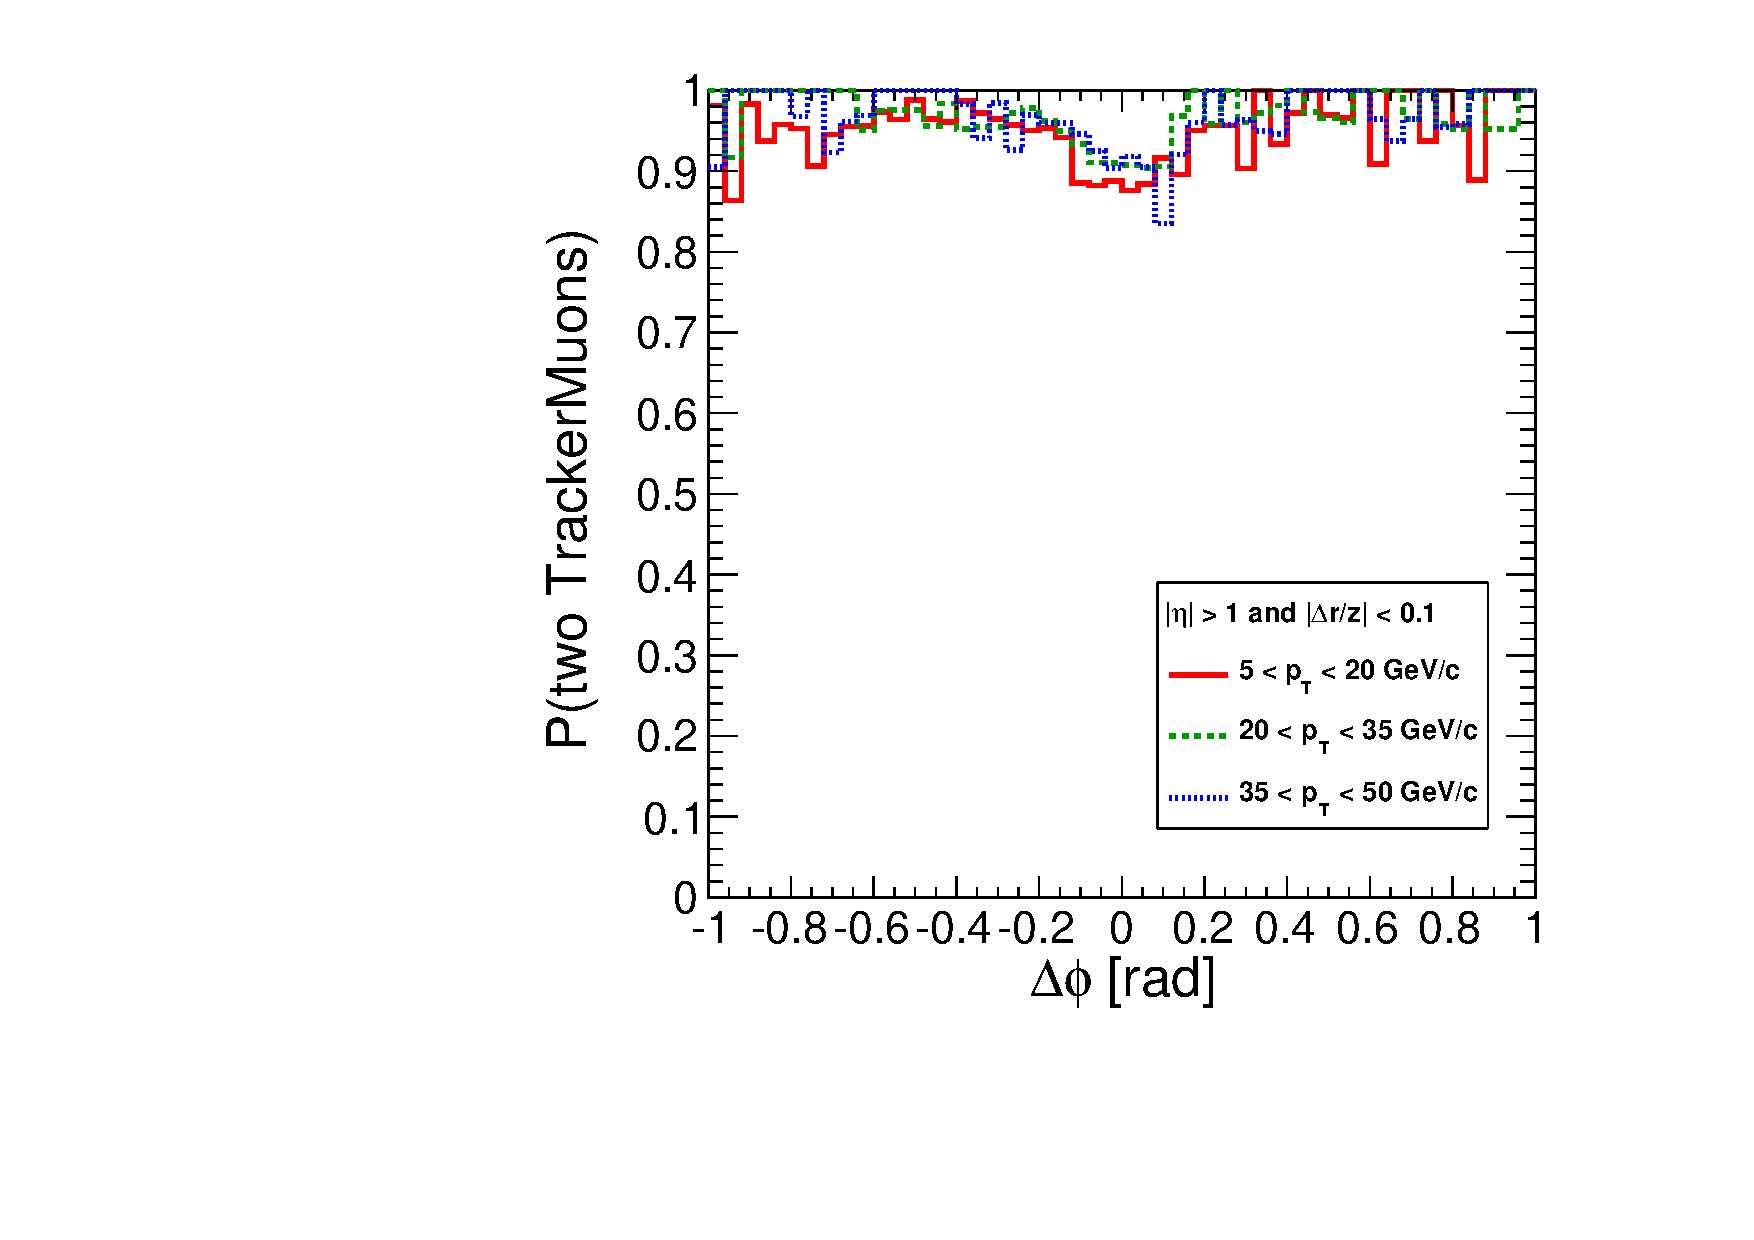
\includegraphics[width=0.48\linewidth]{PLOTS/endcap_dphi_bypt_twoTrackerMuons.pdf}
\caption{Comparison of outside-in (left) and inside-out (right) muon
identification efficiency as a function of the separation of the muon trajectories in the muon system (top: barrel, bottom: endcap). \label{fig:appendix_reconstruction}}
\end{figure}

\section{Muon Trigger Performance for Events with Nearby Muons}
\label{sec:motivation_for_trigger_choice}

There are many reasons why the muon trigger performance may be
affected by the presence of additional muon hits or segments nearby
affecting triggering efficiency for events with multiple nearby or
even crossing (in the muon stations) muons. In the worst-case
scenario, events with a sufficiently energetic muon and additional
nearby muons, there could be no single muon reconstructed by the
trigger or, because of incorrect assignment of segments, the trigger
may reconstruct one or more soft muons below the trigger
threshold. While outside-in reconstruction used in the HLT always
reconstructs the highest $p_T$ muon, it often fails in reconstructing
the second muon if it happens to be nearby. Therefore, selecting such
events using multi-muon triggers (e.g.\ HLT\_DoubleMu3) will lead to a
substantial loss of efficiency even at the HLT level. This was one of
the reasons for this analysis opting for a single-muon trigger, as
outside-in reconstruction guarantees that at least the highest $p_T$
muon candidate is reconstructed. However, apart from HLT, there are
many reasons why the topologies for intersecting muons may be
difficult for the Level-1 muon trigger. Examples of it include the
limitation in the CSC on the maximum number of two trigger stubs per
chamber reported to the CSC Track Finder (CSC-TF), which could lead to
stubs reported to the CSC-TF being a mixture of stubs from different
muons.  Another example is ghost-busting veto at the level of chambers
and in the CSC-TF vetoing duplicate muon candidates. While the latter
effect is likely to mostly affect multi-muon triggers by failing to
reconstruct two nearby muons, the former may affect even the single
muon triggers by not reconstructing any muon candidates above the
trigger threshold.

\begin{figure}[tbh]
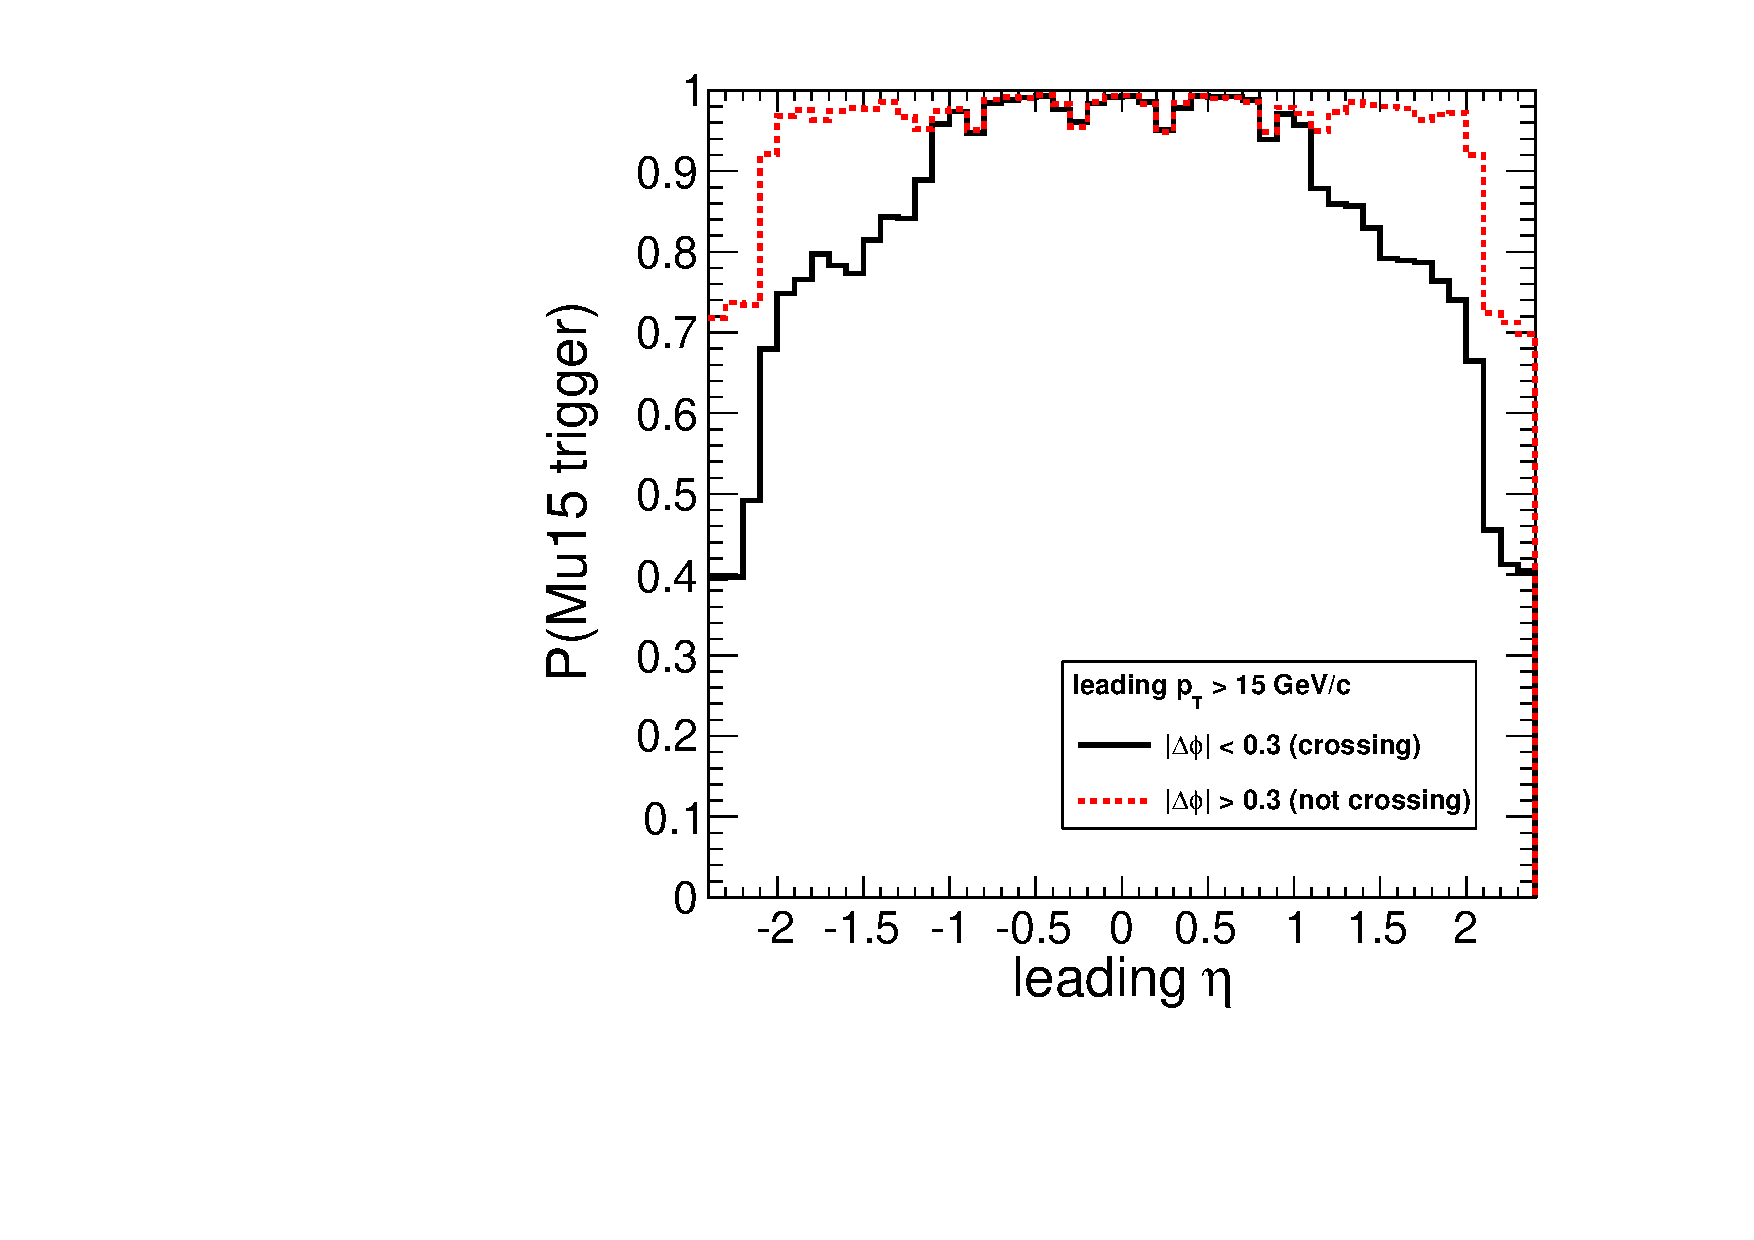
\includegraphics[width=0.32\linewidth]{PLOTS/eta_mass5cut_triggerMu15_nosuppressedzero.pdf} \hfill
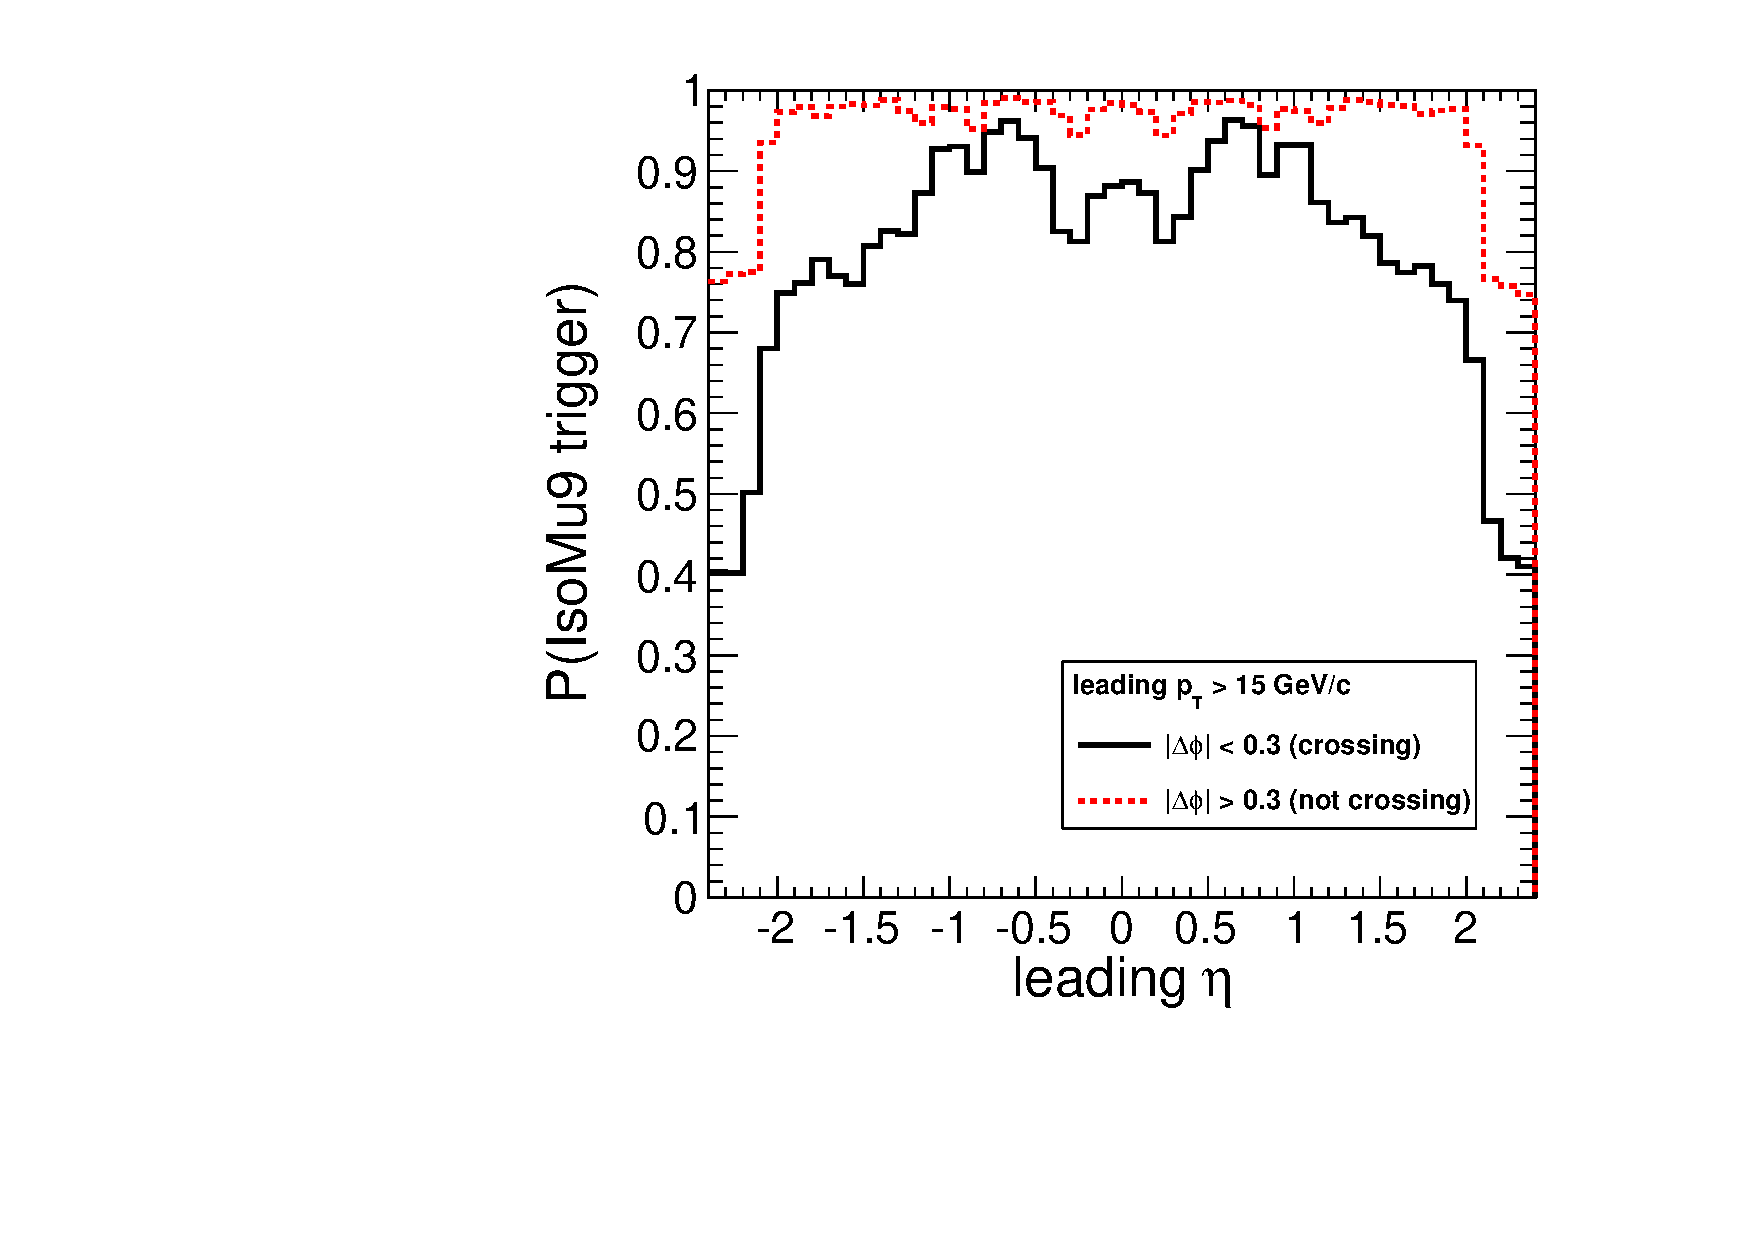
\includegraphics[width=0.32\linewidth]{PLOTS/eta_mass5cut_triggerIsoMu9.pdf} \hfill
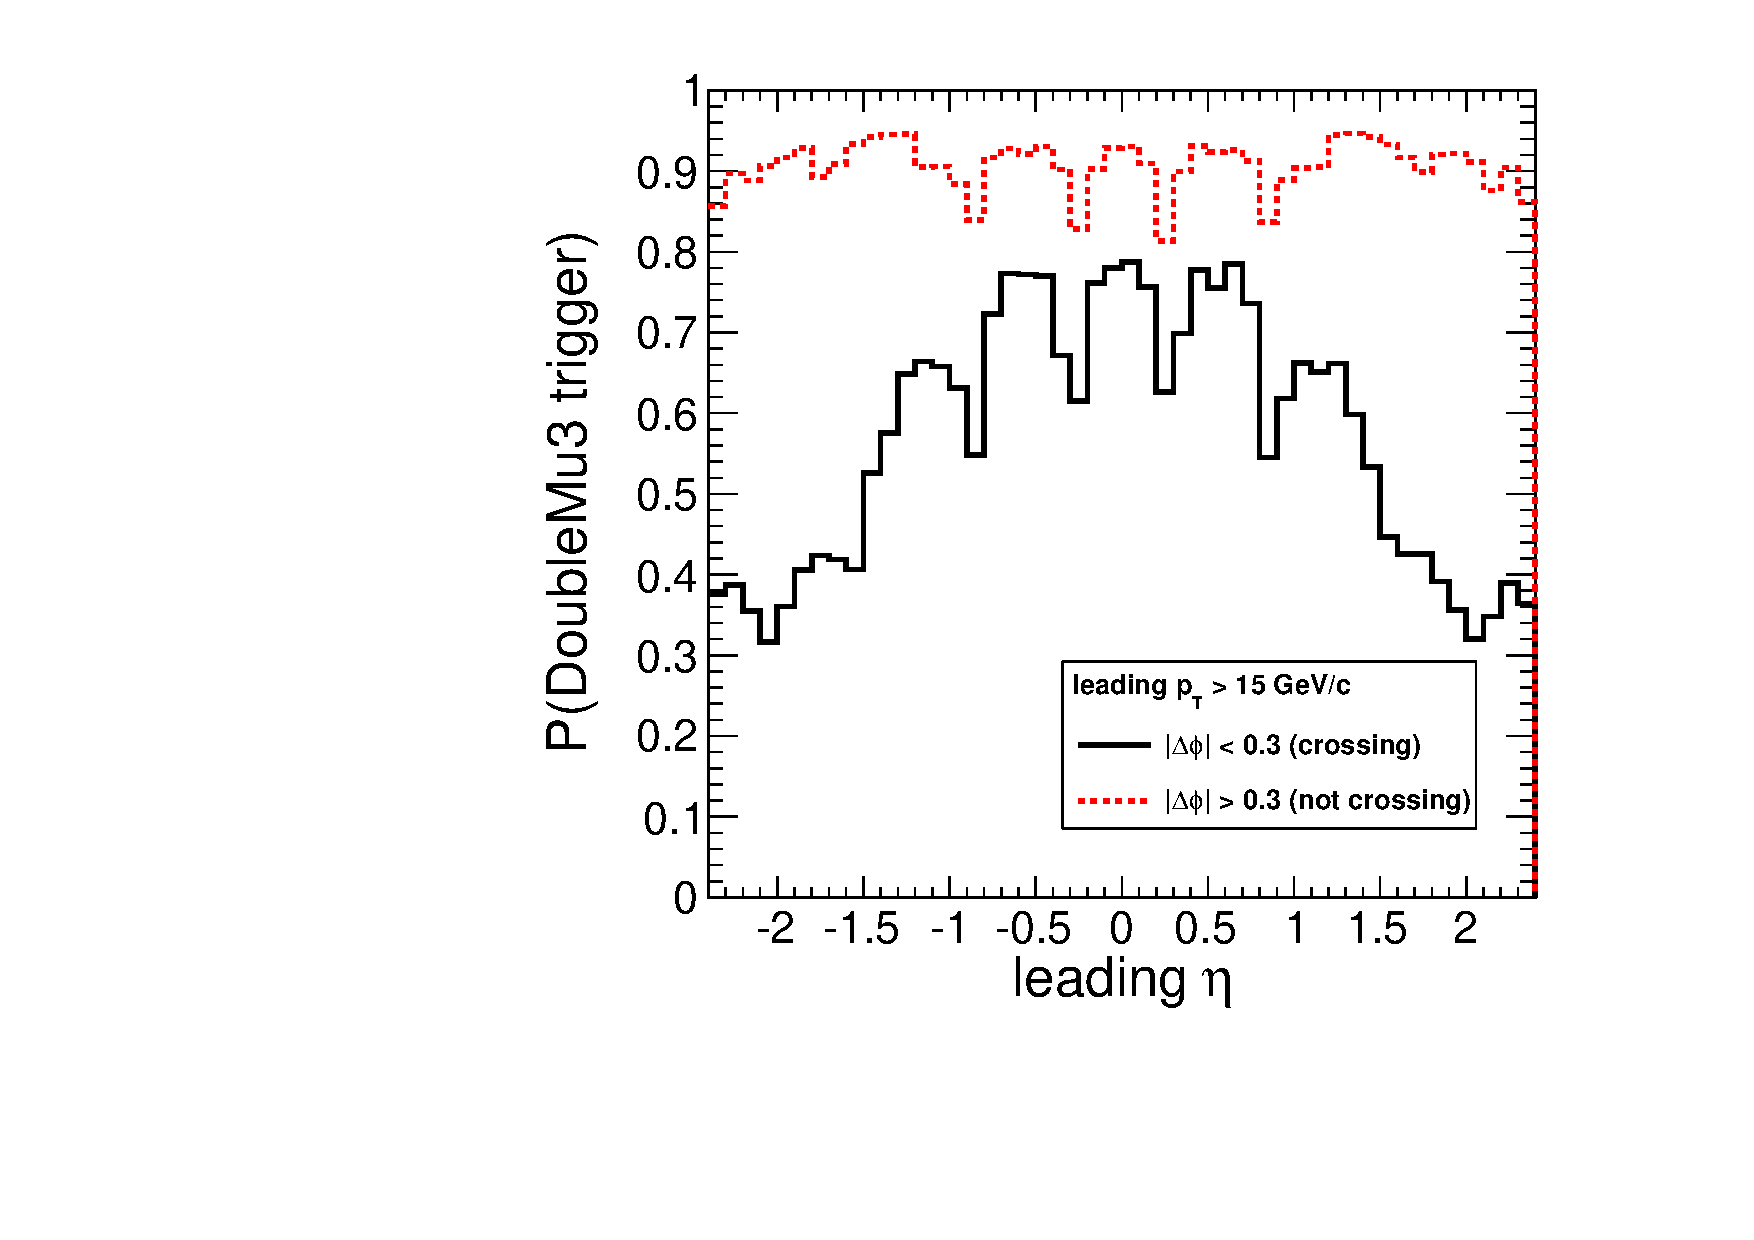
\includegraphics[width=0.32\linewidth]{PLOTS/eta_mass5cut_triggerDoubleMu3.pdf}
\caption{Efficiency of three triggers as a function of $\eta$ and degree of trajectory-crossing in the muon system.  Left: single-muon, unisolated trigger (used within $|\eta| < 0.9$).  Middle: single-muon, isolated trigger (not used).  Right: double-muon trigger (not used). \label{fig:appendix_trigger}}
\end{figure}

To investigate these effects, we used the same sample of simulated
dimuon with a flat dimuon invariant mass distribution and measured
trigger efficiency for single inclusive muon (HLT\_Mu15\_v1), single
isolated muon (HLT\_IsoMu9), and the dimuon (HLT\_DoubleMu3) trigger
configurations. Because the main cause of inefficiency is the
closeness of muons in muon stations, we split the sample into the
``crossing'' and ``not crossing'' samples using $\Delta \phi$ of the
two propagated muon positions at the cylinder and planes described in
Appendix~\ref{sec:motivation_for_reconstruction_methods}. We use trigger
emulation to parameterize efficiency of each trigger using $\eta$ of
the highest $p_T$ muon. The corresponding efficiencies are shown in
Fig.~\ref{fig:appendix_trigger} for the three trigger
configurations. From the comparisons of the ``crossing'' and ``not
crossing'', it is evident that only the inclusive non-isolated
trigger is robust with respect to the presence of additional muon
segments, and only in the barrel region, which determined the
requirement of a trigger muon within $|\eta|<0.9$ in our analysis. The
same trigger develops inefficiency in the overlap and endcap region,
likely because of the confusion in selecting segments used in building
a track and the effects of the ``ghost-busting'' procedure in the
CSC-TF. The isolated trigger shown in Fig.~\ref{fig:appendix_trigger}(b),
is also developing inefficiency for ``crossing'' topology in the
entire range due to the second muon interfering with the isolation
requirements. Finally, as shown in
Fig.~\ref{fig:appendix_trigger}(c), the dimuon configuration suffers
the largest inefficiency for the ``crossing'' topology as in this case
the requirement is that both outside-in muon candidates are to be found. The
reduction in efficiency for the ``not crossing'' topology is because
the efficiency in this case is a product of trigger efficiencies for
both legs and the inefficiency in reconstructing the second muon
reduces the overall ``plateau'' efficiency. These observations show
that the the CSC muon trigger algorithm performance deteriorates
significantly\footnote{This study was performed with a 2010B-like
endcap trigger simulation--- no ME1/1 singles and modified ghost
suppression--- though the conclusion is the same for the 2010A-like
endcap trigger simulation.} in the presence of nearby muons even when
the requirement is to reconstruct at least one (high-$p_T$) muon. Both
DT and CSC dimuon trigger efficiencies show large degradation if the
two muons are close to one another and the requirement is to
reconstruct both muon candidates.

While the above addresses the algorithmic part of the muon trigger
performance in the presence of additional nearby muons, another source
of trigger inefficiency is due to generic instrumental effects. These
include accuracy in simulating the response of the chambers in the
fiducial volume and on edges in terms of stub reconstruction
efficiency, reduction in efficiency due to dead regions, masked
channels etc. These effects are not correlated with the presence of
additional nearby muons and are universal. Therefore, we correct for
the difference between simulation predictions and actual efficiency in
the data using a single scale factor for inclusive muon trigger
efficiency based on the measurement derived in
Appendix~\ref{sec:tag_and_probe}, below.

Based on these observations, we conclude that since the masses and
momentum distributions of new physics dimuons is unknown, the endcap
trigger efficiency cannot be quantified easily without parameterizing
efficiency in both of these variables, which will substantially
complicate the analysis and later interpretation of the results.  That
is why we require at least one above-threshold muon in the barrel per
event.

\section{Trigger Efficiency Correction from Tag-and-Probe}
\label{sec:tag_and_probe}

To account for differences between the simulated trigger efficiencies
and the real trigger efficiency, we performed a tag-and-probe study of
our datasets with the $Z\to\mu\mu$ resonance and consulted similar
studies from other CMS analyses.\footnote{Summary of muon trigger
efficiency in $t\bar{t}$ cross-section studies:
\href{https://twiki.cern.ch/twiki/bin/view/CMS/TopLeptonPlusJetsEffStudies}{https://twiki.cern.ch/twiki/bin/view/CMS/ TopLeptonPlusJetsEffStudies}
and especially Sin\'ead Walsh's talk at the Muon HLT POG:
\href{http://indico.cern.ch/conferenceDisplay.py?confId=122082}{http://indico.cern.ch/ conferenceDisplay.py?confId=122082}.  These
studies find an HLT\_Mu9 scale factor of $0.94/0.97 = 0.969 \pm 0.002$
and an HLT\_Mu15 scale factor of $0.955/0.97 = 0.985 \pm 0.002$ in the
$|\eta| < 0.9$ barrel region.}  We selected two offline muons passing
our selection criteria (Sec.~\ref{sec:reconstruction_and_efficiency}),
as well as $p_T > 15$~GeV/$c$.  We designated one muon as a tag and
required it to be in the endcap with $1.2 < |\eta| < 2.1$ and matched to a
$p_T > 15$~GeV/$c$ trigger object (Level-3), thereby satisfying the
trigger.  The other muon, designated as probe, was required to have
$|\eta| < 0.9$.  We call this sample of events the denominator.  If,
in addition to these requirements, the probe also matched a Level-3
$p_T > 15$~GeV/$c$ trigger object, the event belongs to a numerator
sample.  The denominator and numerator samples were independently
background-subtracted using the sidebands shown in
Fig.~\ref{fig:triggeff_tagandprobe} and a linear background shape.
The number of events in the background-subtracted numerator divided by
the number of events in the background-subtracted denominator is taken
to be the efficiency of the single-muon trigger with $p_T >
15$~GeV/$c$, $|\eta| < 0.9$ (a combination of HLT\_Mu9 and HLT\_Mu15
with kinematic cuts on the Level-3 muon to emulate 15~GeV/$c$ for the
whole dataset).  Results are shown in
Fig.~\ref{fig:triggeff_tagandprobe}.  This study was performed for the
dataset used in this analysis and a Monte Carlo sample generated in
the same software version as the Monte Carlo samples used to calculate
efficiencies for this analysis.  The data-over-MC ratio, $0.947/0.978$
implies a $0.968 \pm 0.006$ scale factor, in agreement with studies
performed by other CMS groups.

\begin{figure}
\begin{center}
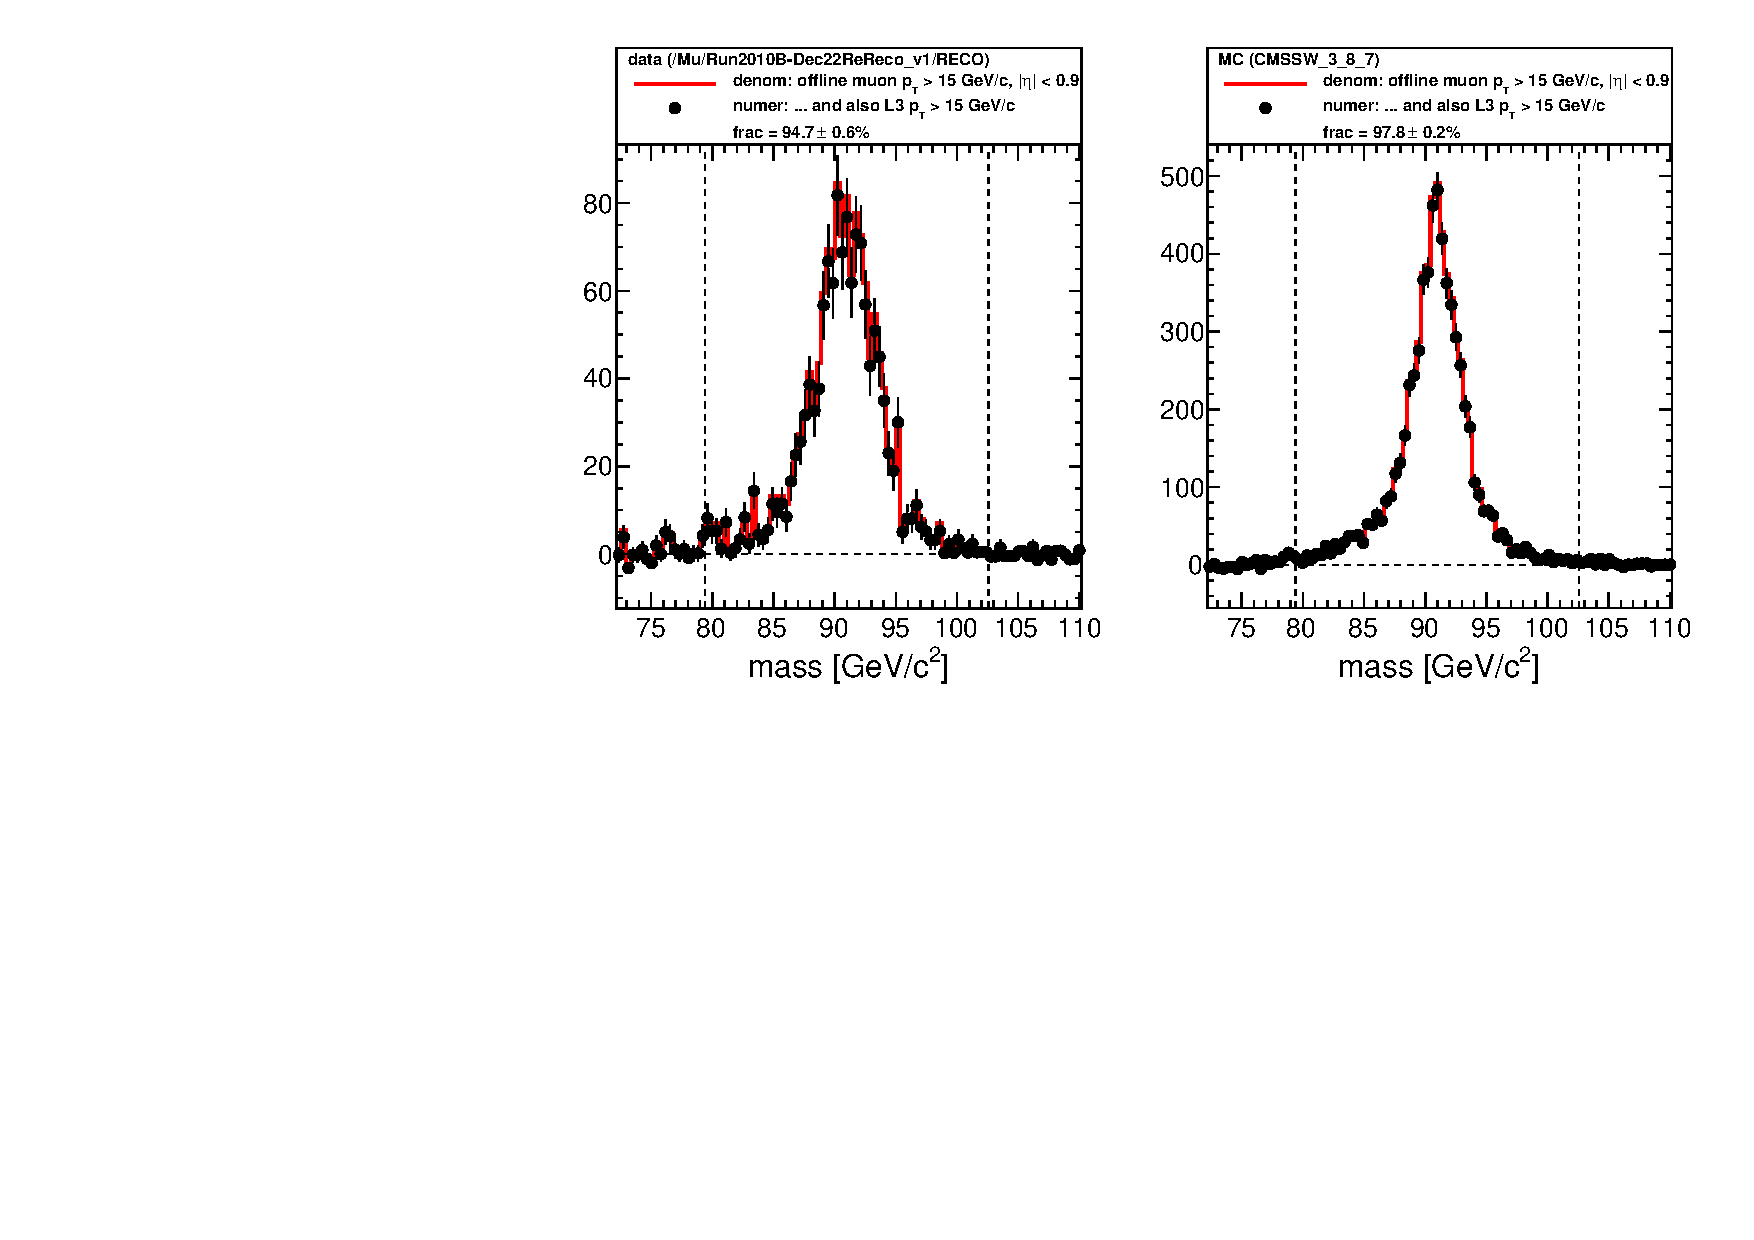
\includegraphics[width=0.8\linewidth]{PLOTS/trigeff_endcapbarrel_0968.pdf}
\end{center}

\caption{$Z\to\mu\mu$ events with and without a $p_T > 15$~GeV/$c$ trigger object matched to the probe muon.  Sidebands beyond the dashed lines were used to subtract non-resonant backgrounds.  Left: dataset used for the analysis.  Right: Monte Carlo generated in the same software release as all efficiency measurements.  See text for details. \label{fig:triggeff_tagandprobe}}
\end{figure}

The tag and probe are required to be in non-overlapping regions of the
detector (endcap and barrel, respectively) to ensure that their
trajectories do not cross in the muon system.  We know from studies in
Appendix~\ref{sec:motivation_for_reconstruction_methods} that the
outside-in muon identification algorithm is highly inefficient for
muons that cross (about 50\%, depending on closeness and $p_T$), and
the muon identification used by the software trigger is outside-in.
If a fraction of the tag and probe muons cross ($x$
= \#crossing/\#total), then the efficiency measured by tag-and-probe
would be lower than the true single-muon efficiency (tag-and-probe
would measure $[0.5 x + (1-x)] \varepsilon$ instead of the true
efficiency, $\varepsilon$).  Since $Z$ bosons are produced with
relatively little boost, the muons from $Z\to\mu\mu$ decays rarely
overlap ($x \lesssim 0.1$\%), in addition to providing muons with
momenta relevant to our signal search ($p_T \approx$ tens of GeV/$c$).
The tag and the probe do not strictly need to be in different
subsystems to avoid bias from overlaps: we know from
Fig.~\ref{fig:appendix_reconstruction} that a sufficient condition to
avoid overlaps in the barrel is
\begin{equation}
(\Delta \phi < -0.4 \mbox{ \bf or } \Delta \phi > 1) \mbox{ \bf and } |\Delta z / r| > 0.3.
\end{equation}
Repeating the efficiency study with this cut to avoid overlaps instead
of requiring the tag to be in the endcap yields a scale factor of
$94.2/97.7 = 0.964 \pm 0.004$, a systematic difference from the first
study which is smaller than the statistical uncertainty.

Tag-and-probe studies of offline selection efficiency performed
by other CMS groups yield data/MC scale factors of $1.000 \pm 0.003$,
so we did not repeat them for our datasets.

\section{Signal Shape Studies Using Low Mass Resonances in Data}
\label{sec:appendix_signal_shape_studies}

Because the shapes of the dimuon invariant mass distributions are completely determined by detector resolution effects (dominated by tracking), these shapes can be obtained from actual low mass resonances directly in data. The studies in data are compared to Monte Carlo predictions and we use these comparisons to detemine evolution of the resolution parameters. 

We used the same dataset as in our analysis selections, but to avoid unblinding our signal regions, selected events were required to contain exactly two muons with the transverse momentum of the dimuon system $p_T < 80$~GeV/$c$. Additionally, we expanded the requirement of at least one muon with $p_T > 15$~GeV/$c$ to be within $|\eta| < 2.4$ (as opposed to $|\eta|<0.9$ in the main analysis) to include dimuons reconstructed in the overlap or endcap regions and correspondingly dropped the requirement of a central muon in the trigger selections. This is justified because resolutions are driven by tracking and not by muon or muon trigger performance. We then focus on the regions in the dimuon invariant mass spectrum around the four relevant resonances: $\omega$, $\phi$, $J/\psi$, and $\psi^\prime$. The distributions for the selected data events are shown in Fir.~\ref{fig:respeak_fits} separately for barrel ($|\eta|<0.9$) and forward $|\eta|>0.9$ as resolutions in these regions are different.

\begin{figure}[p]
\centering
\begin{tabular}{cccc}
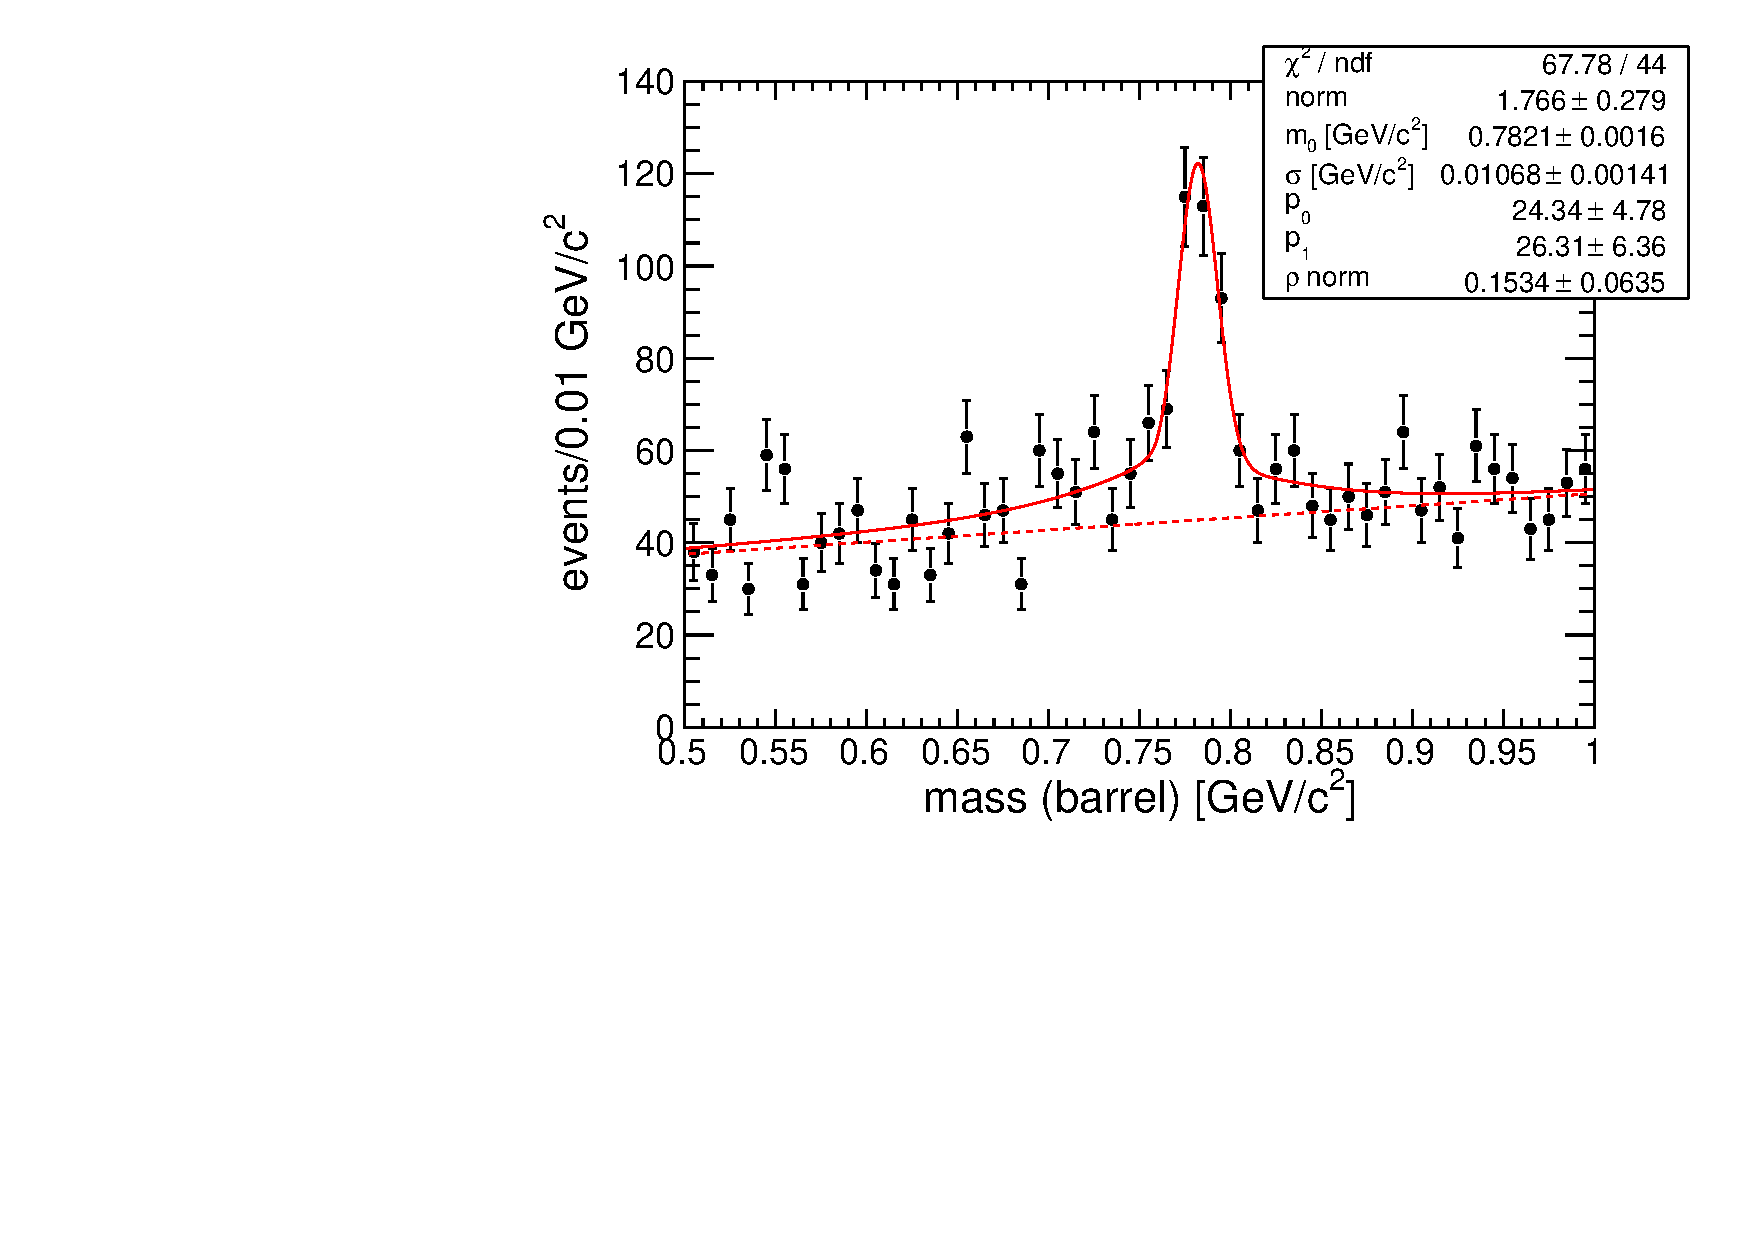
\includegraphics[width=0.48\linewidth]{PLOTS/respeak_omega_barrel.pdf} \hfill
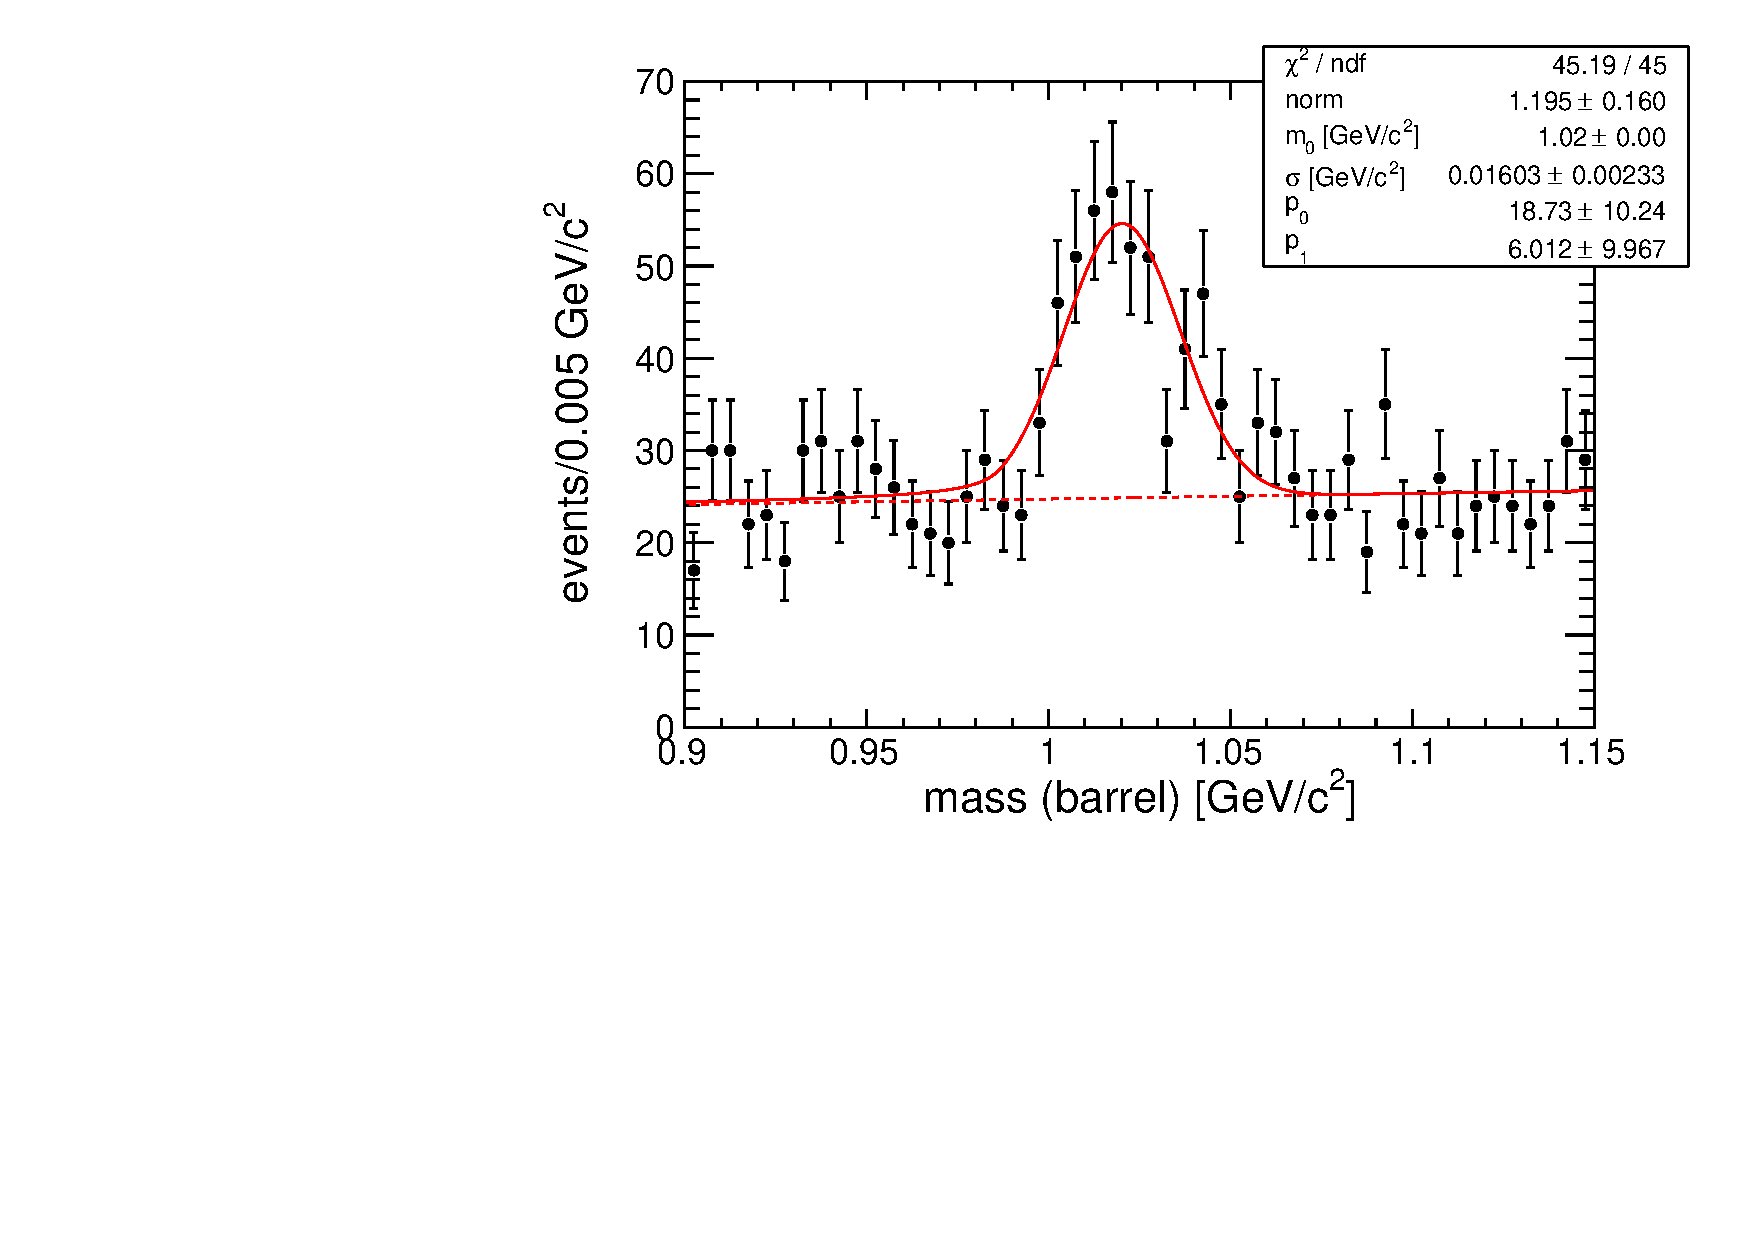
\includegraphics[width=0.48\linewidth]{PLOTS/respeak_phi_barrel.pdf} \\
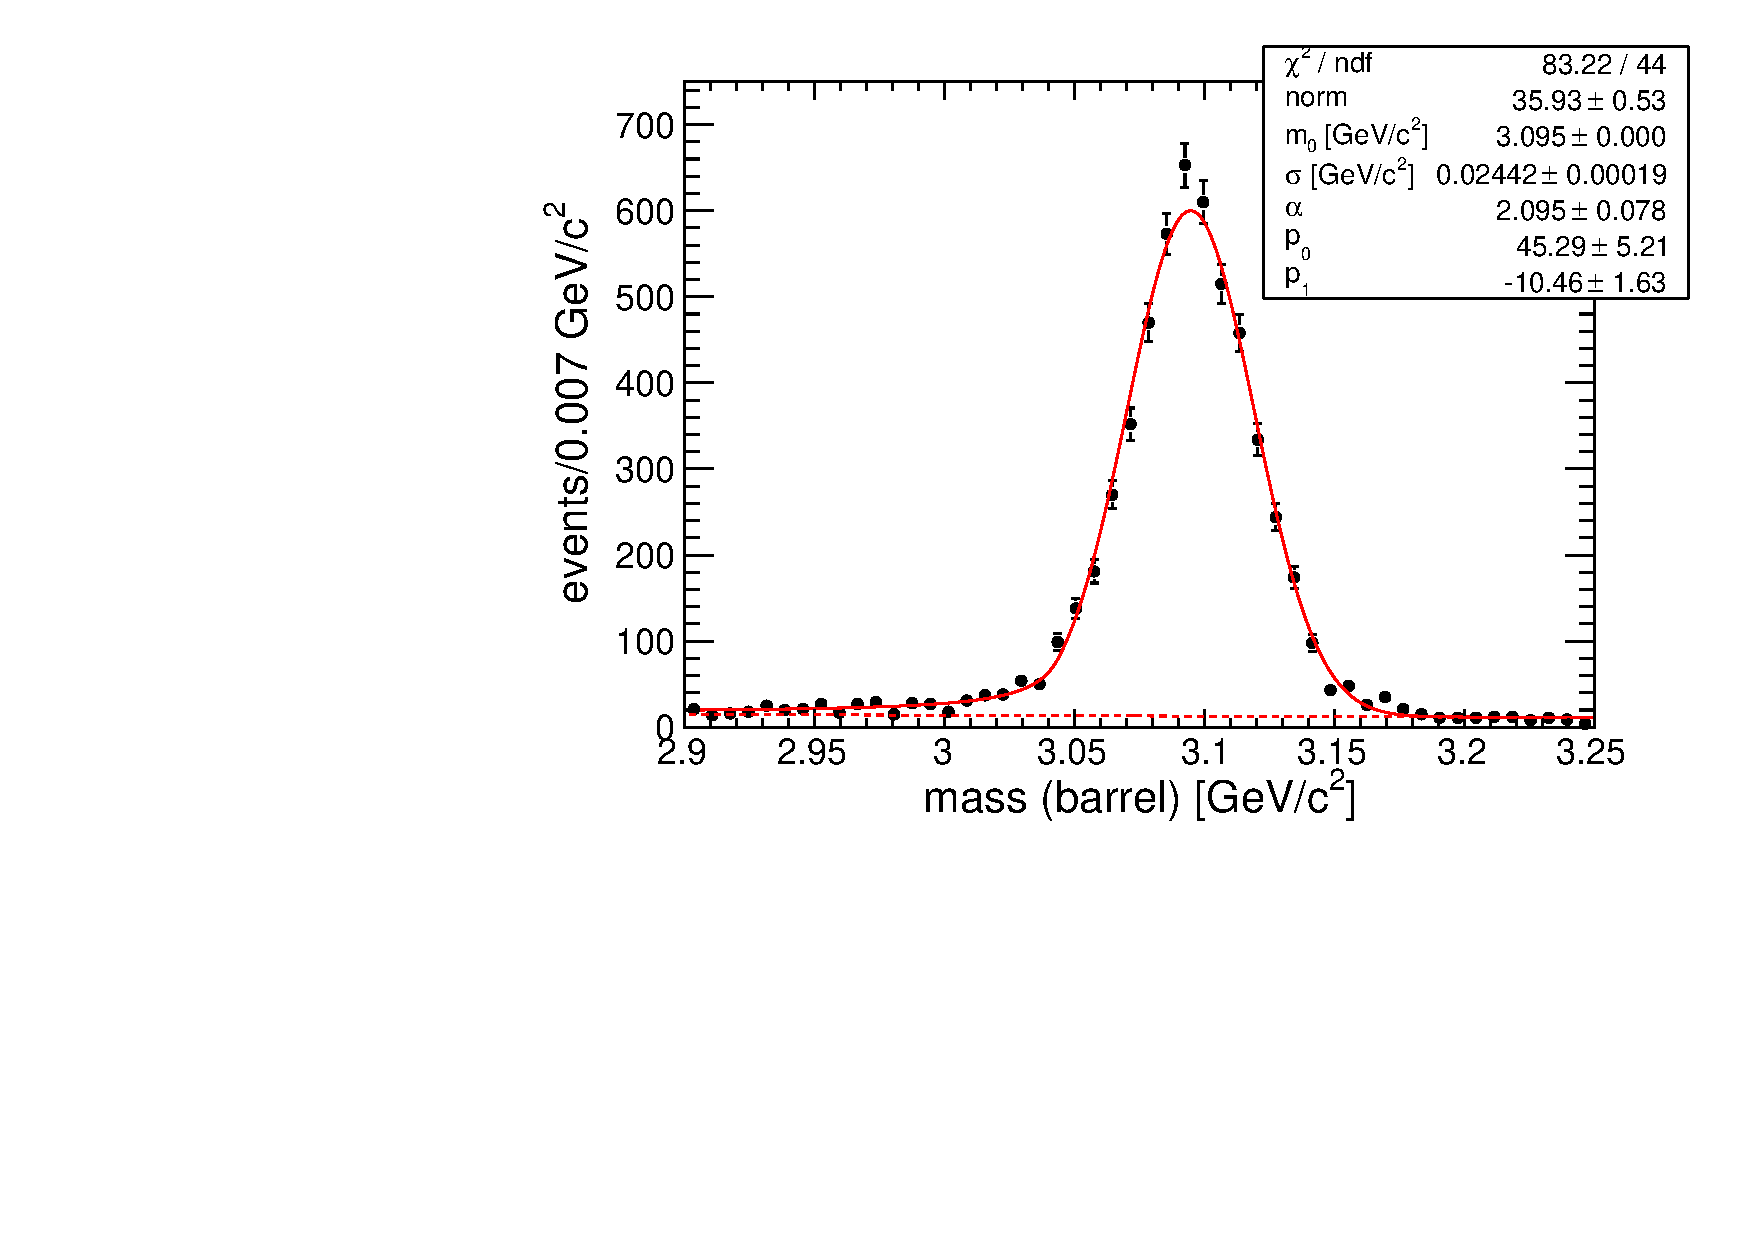
\includegraphics[width=0.48\linewidth]{PLOTS/respeak_jpsi_barrel.pdf} \hfill
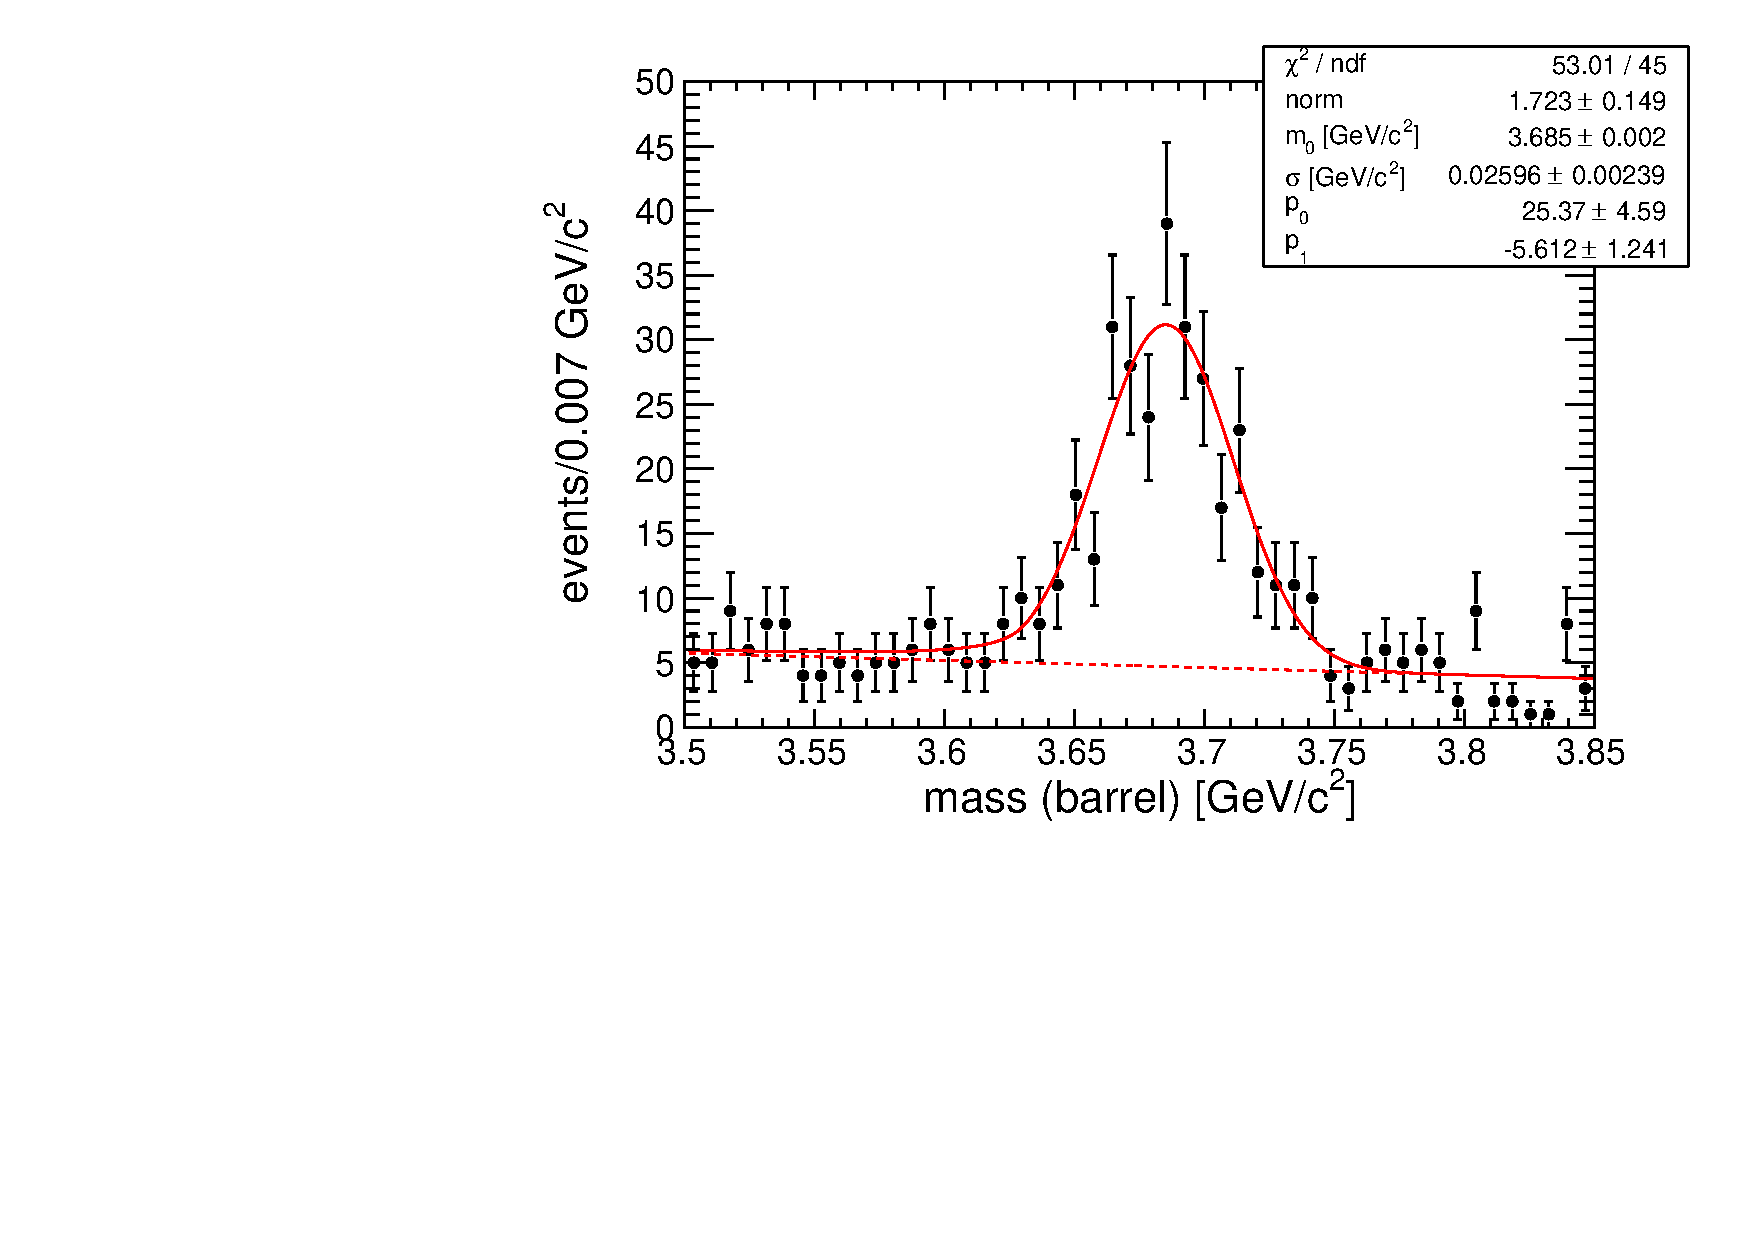
\includegraphics[width=0.48\linewidth]{PLOTS/respeak_psiprime_barrel.pdf} \\
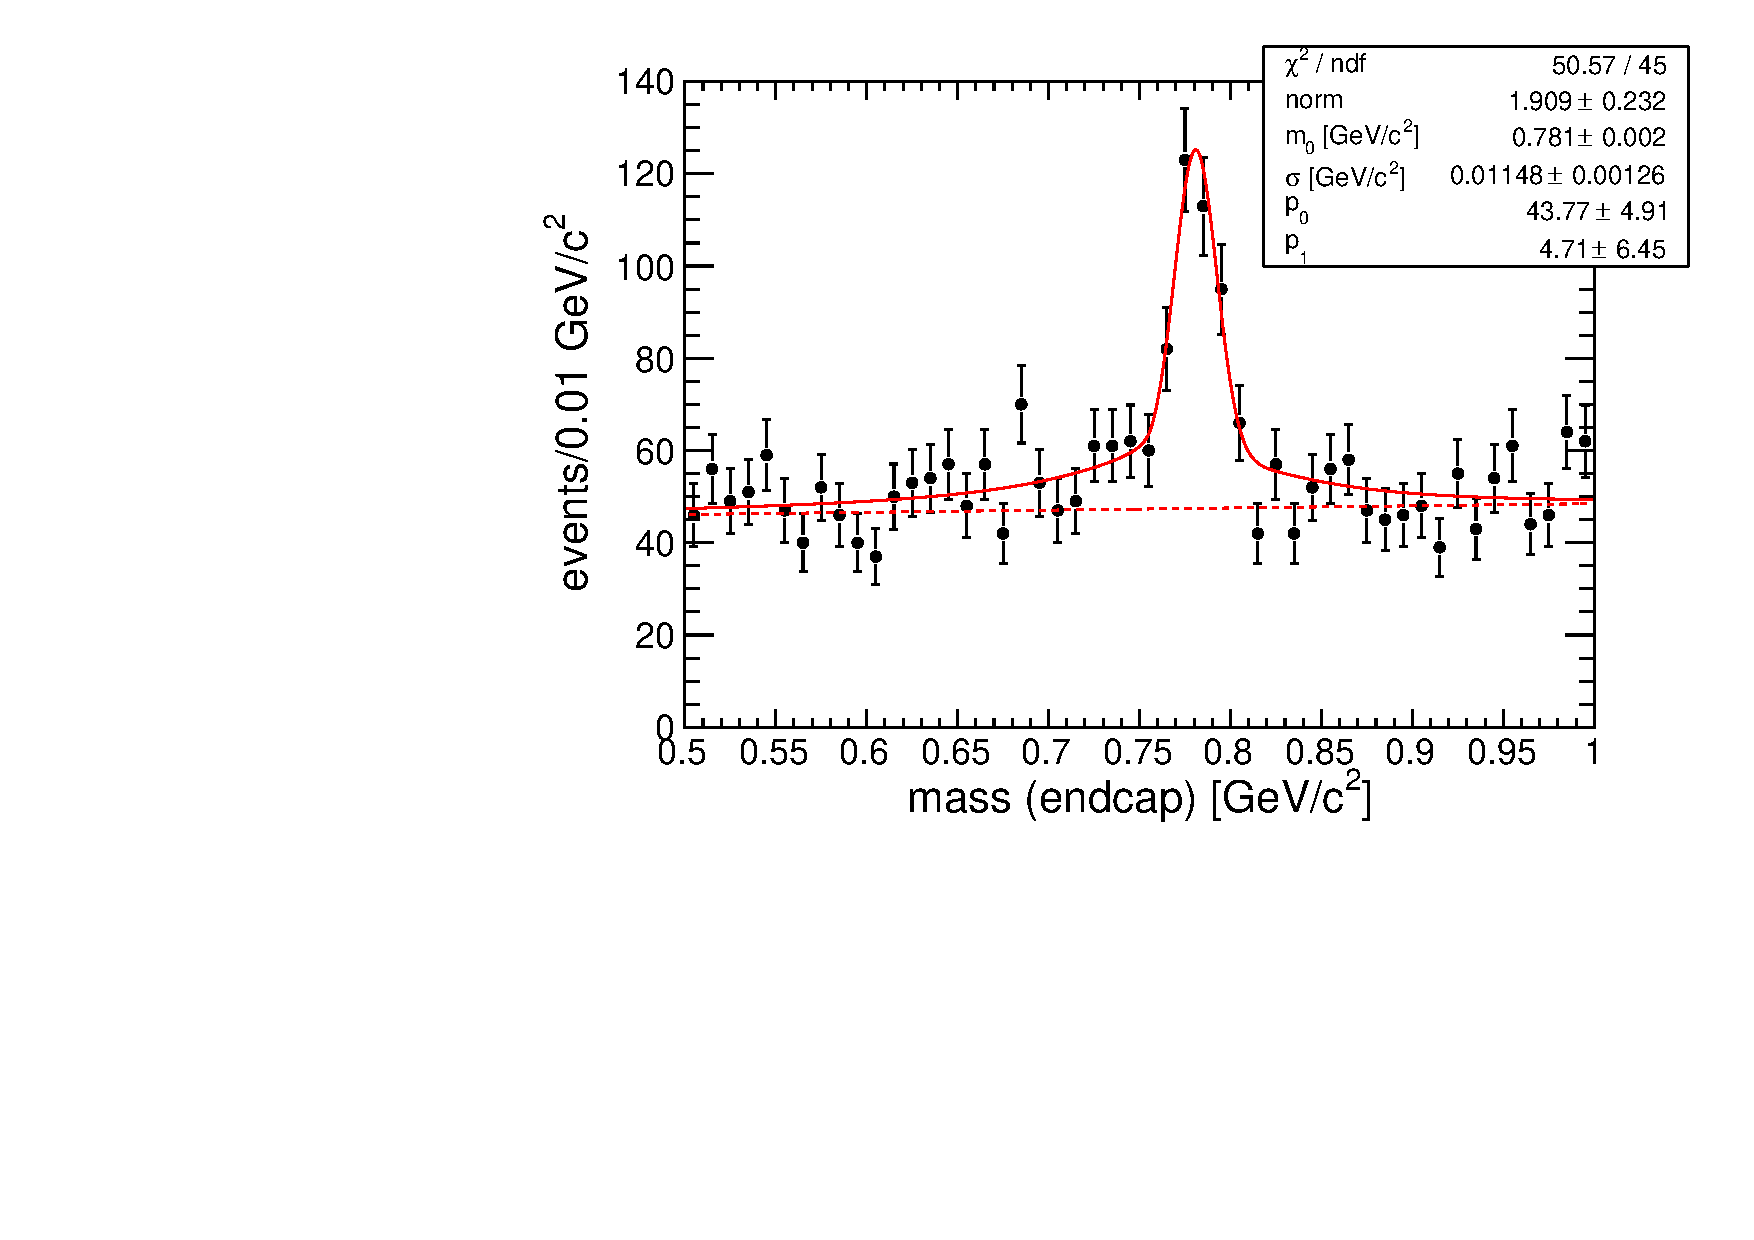
\includegraphics[width=0.48\linewidth]{PLOTS/respeak_omega_endcap.pdf} \hfill
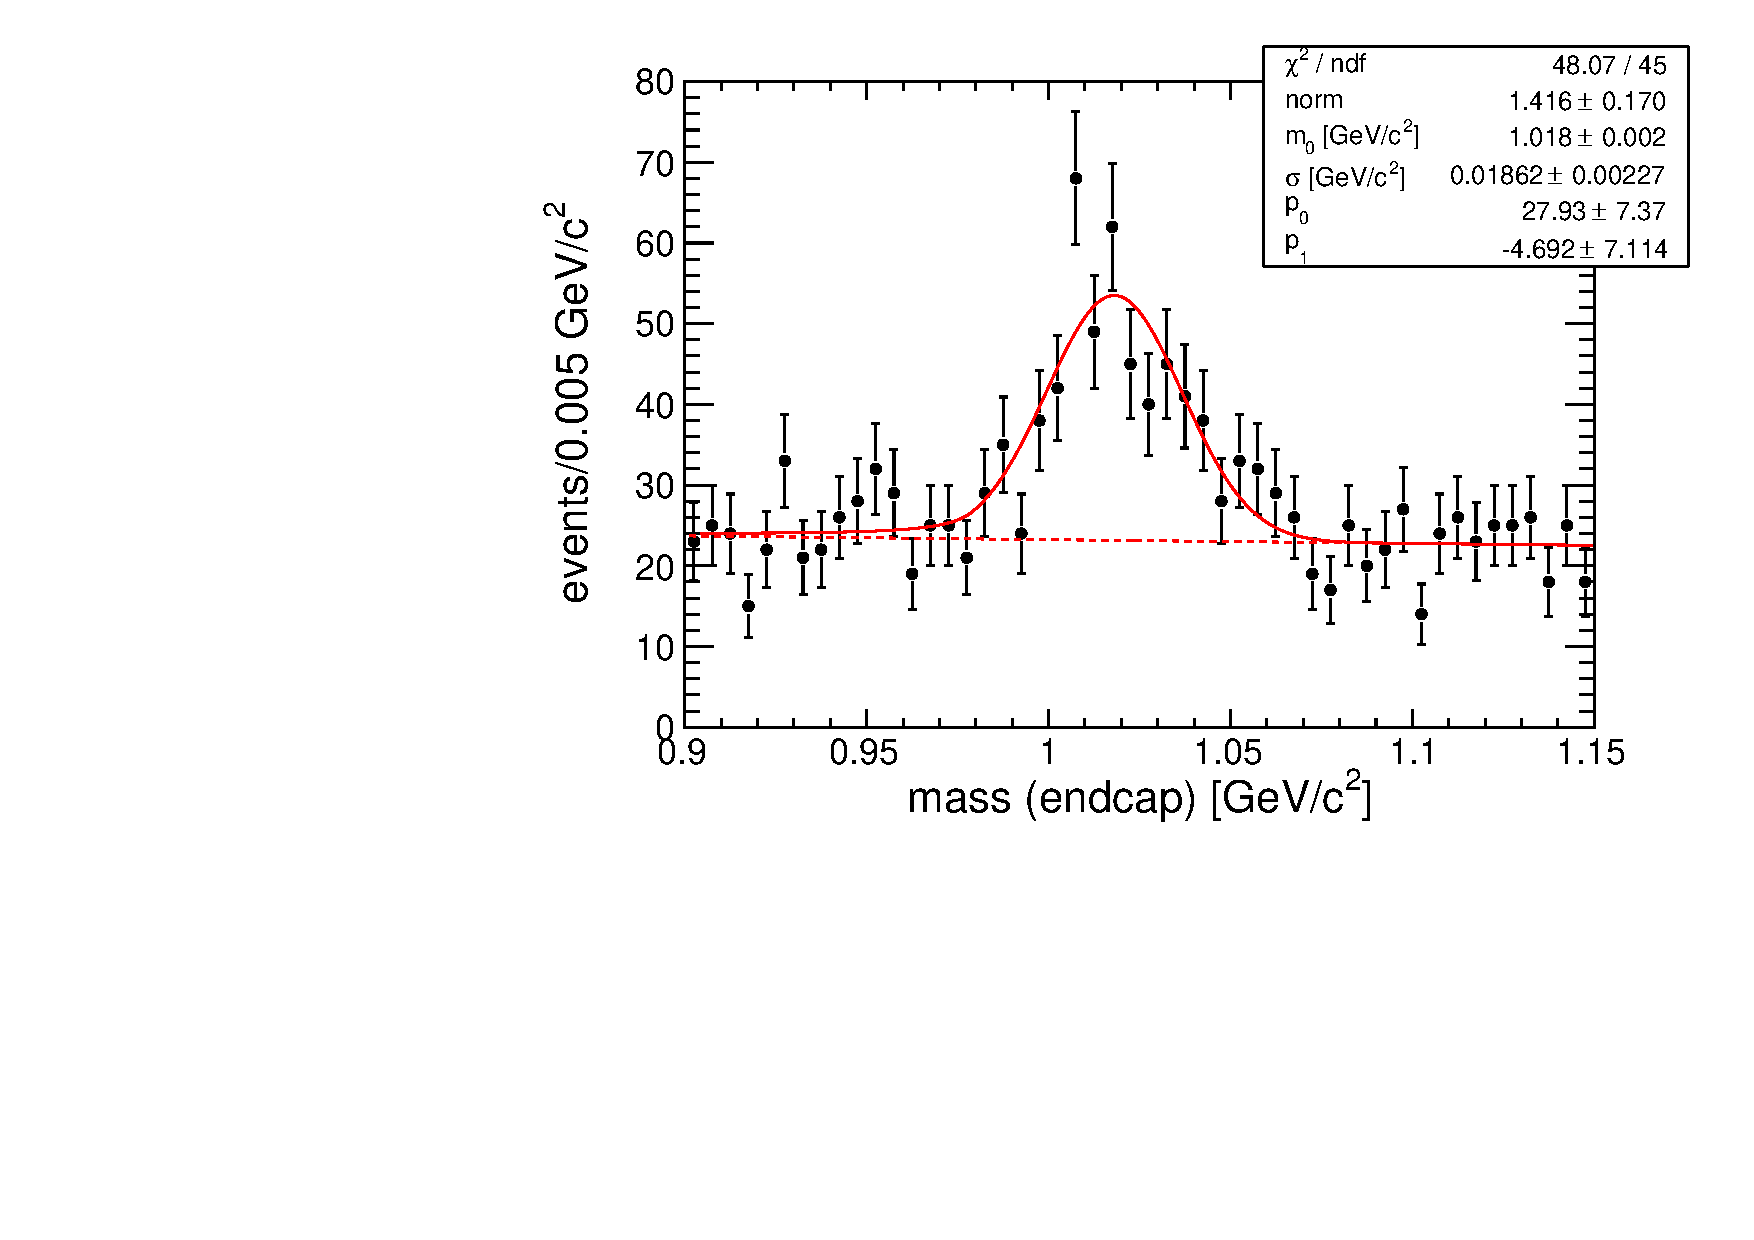
\includegraphics[width=0.48\linewidth]{PLOTS/respeak_phi_endcap.pdf} \\
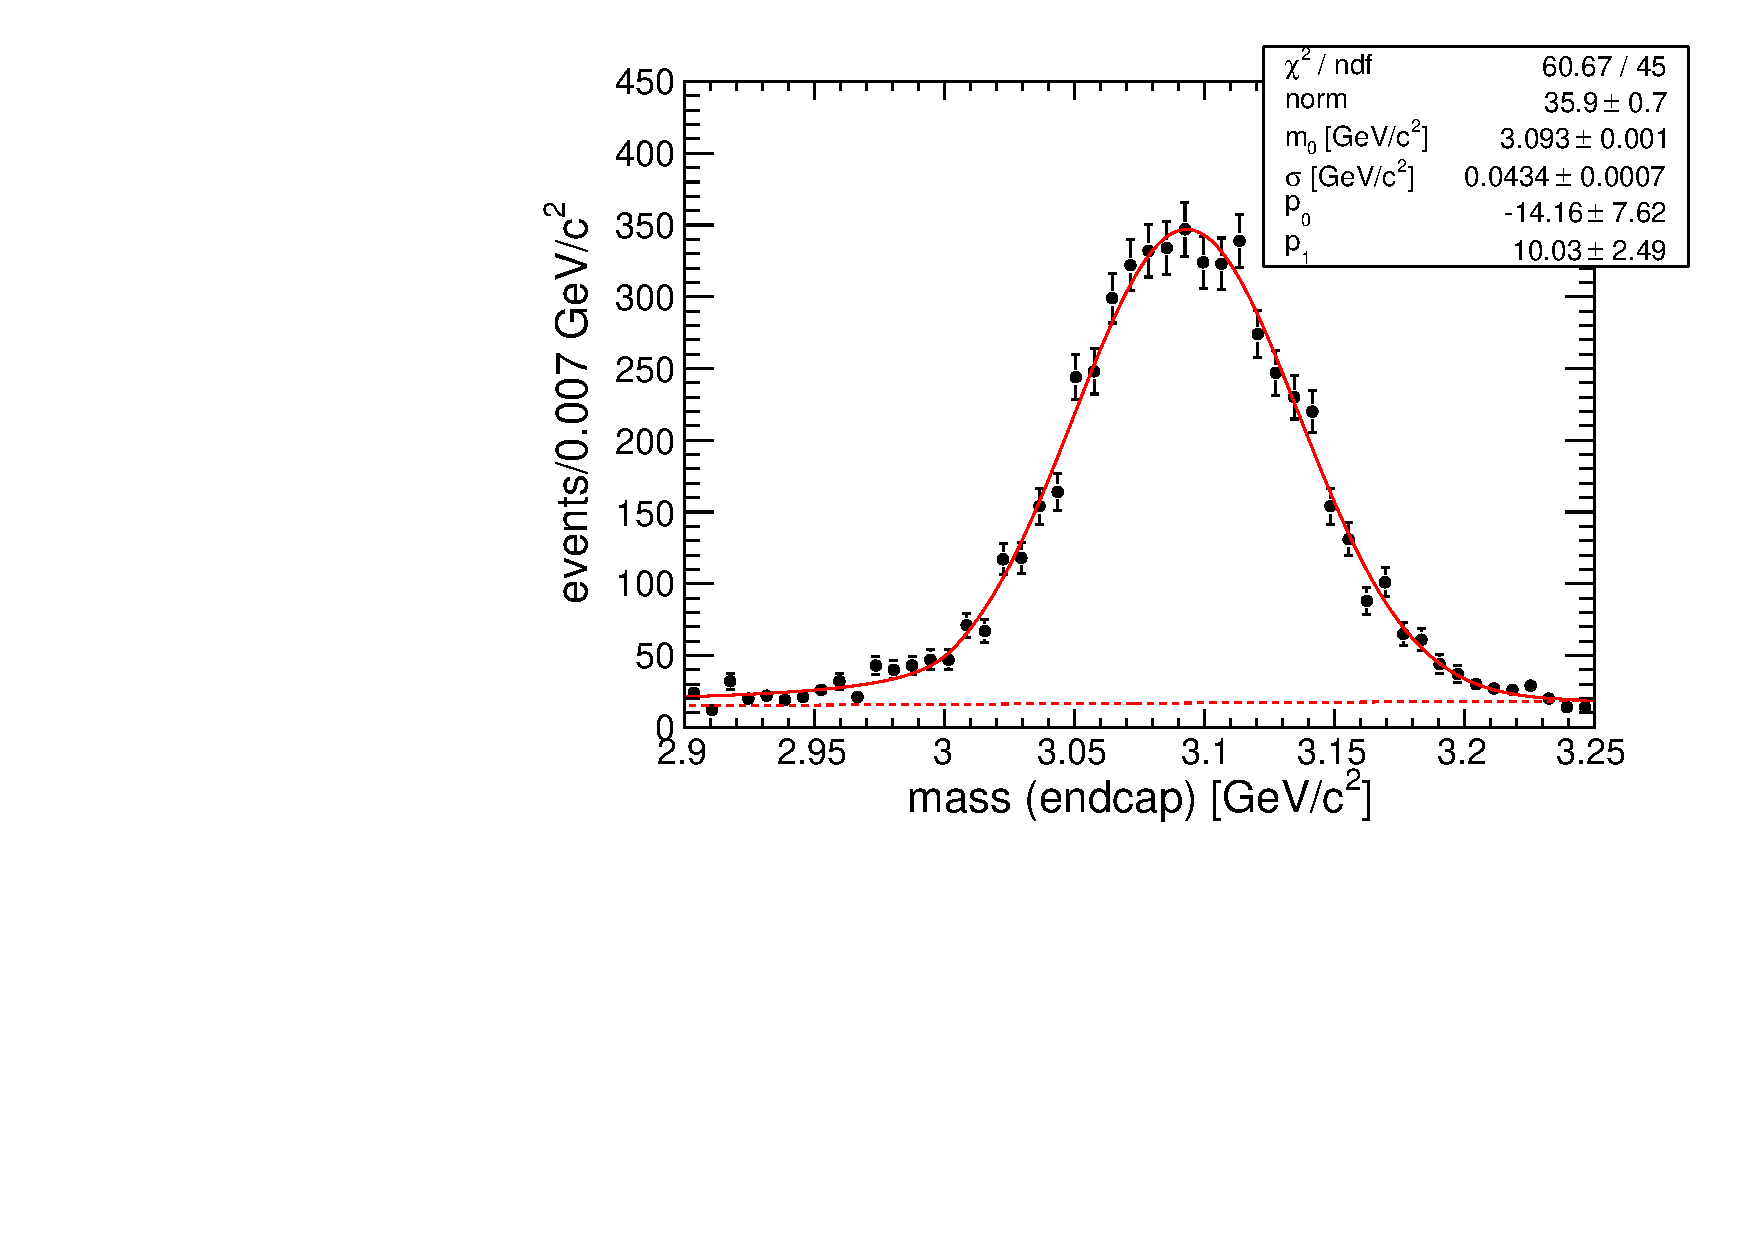
\includegraphics[width=0.48\linewidth]{PLOTS/respeak_jpsi_endcap.pdf} \hfill
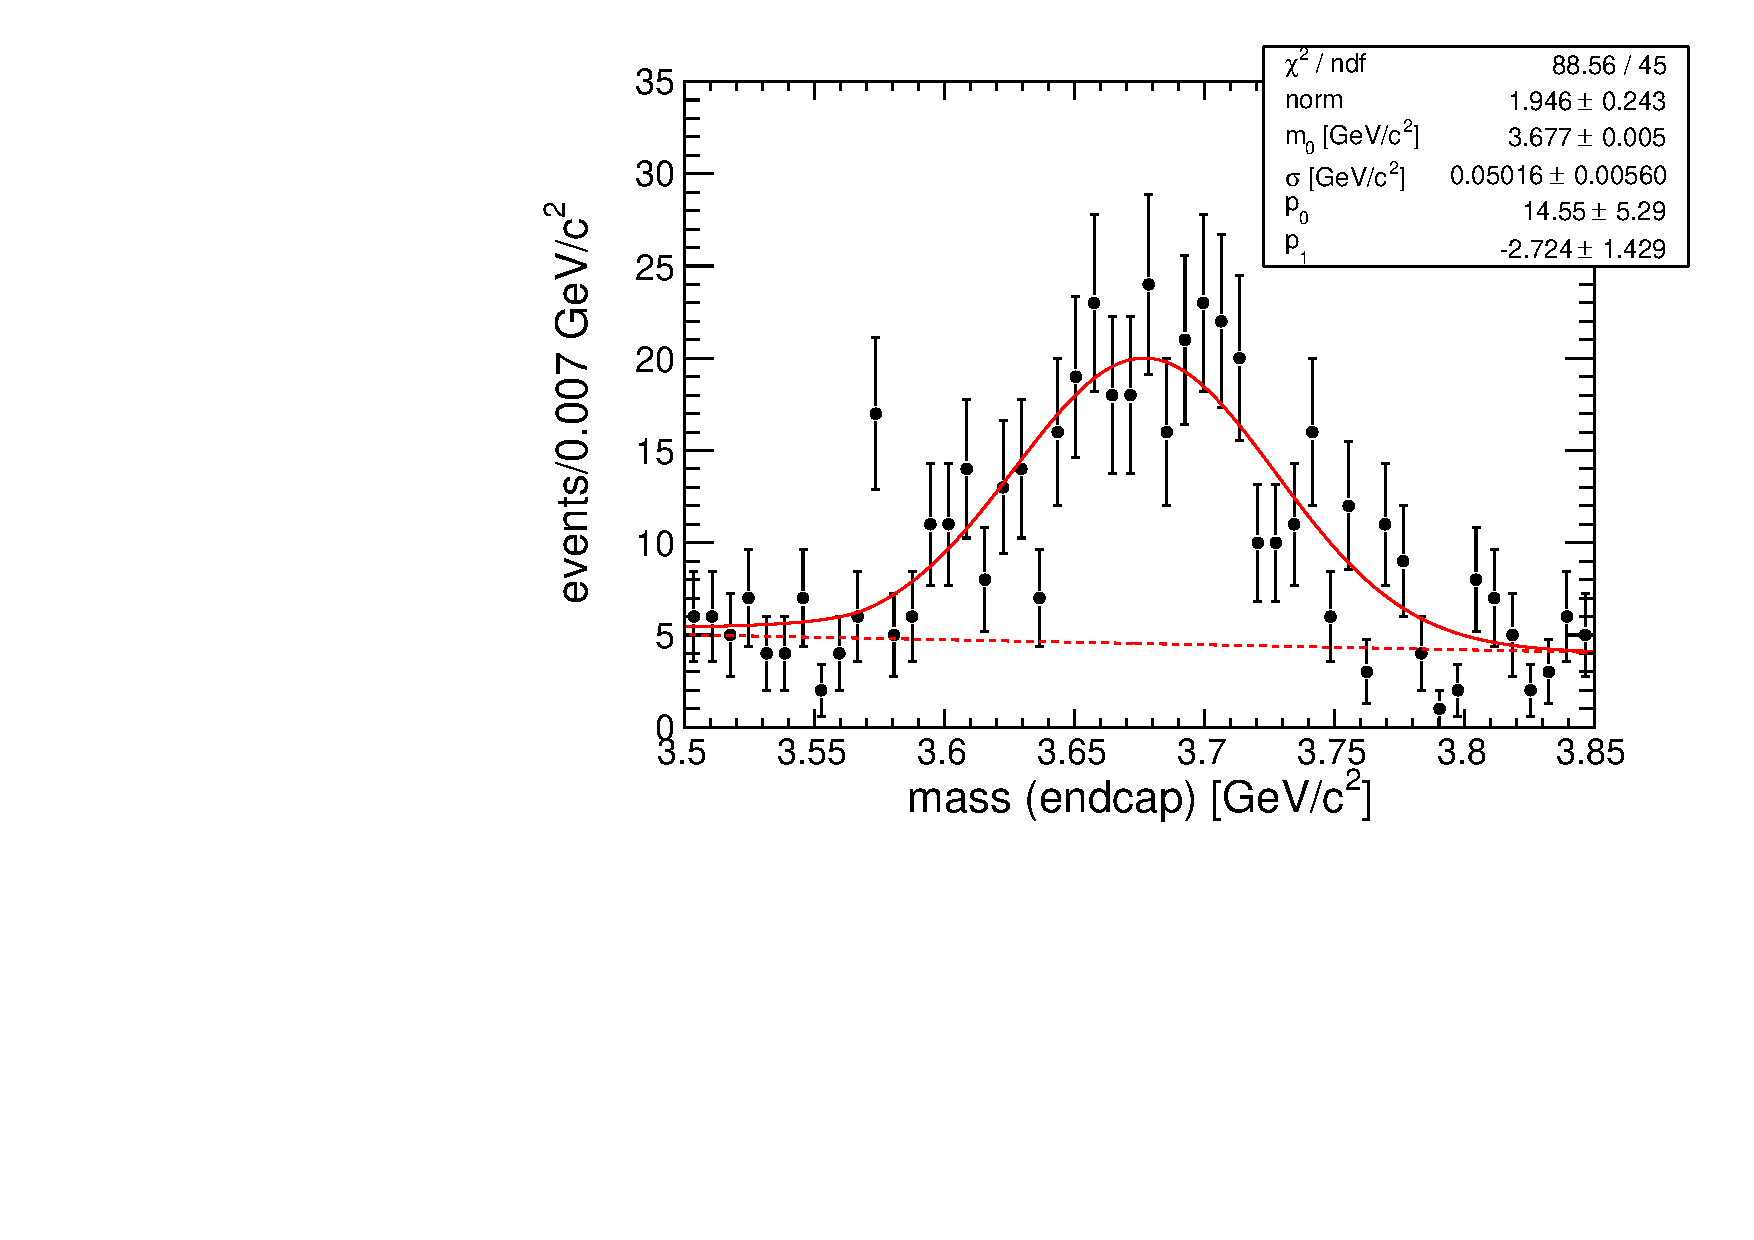
\includegraphics[width=0.48\linewidth]{PLOTS/respeak_psiprime_endcap.pdf} \\
\end{tabular}
\caption{Four resonance mass peak fits in dimuon data: $\omega$, $\phi$, $J/\psi$, and $\psi'$
 in the barrel region $|\eta|<0.9$ (top four plots) and the overlap and endcap $|\eta|>0.9$ (bottom four).  
Signal shapes are fitted to Crystal Ball function with $\alpha$
parameter floating only in the $J/\psi$ barrel case.  Backgrounds are
linear, and the $\omega$
fit has an additional $\rho$ background component with $\rho$ mass and width
taken from the PDG. \label{fig:respeak_fits}}
\end{figure}

\begin{figure}[p]
\centering
\begin{tabular}{c}
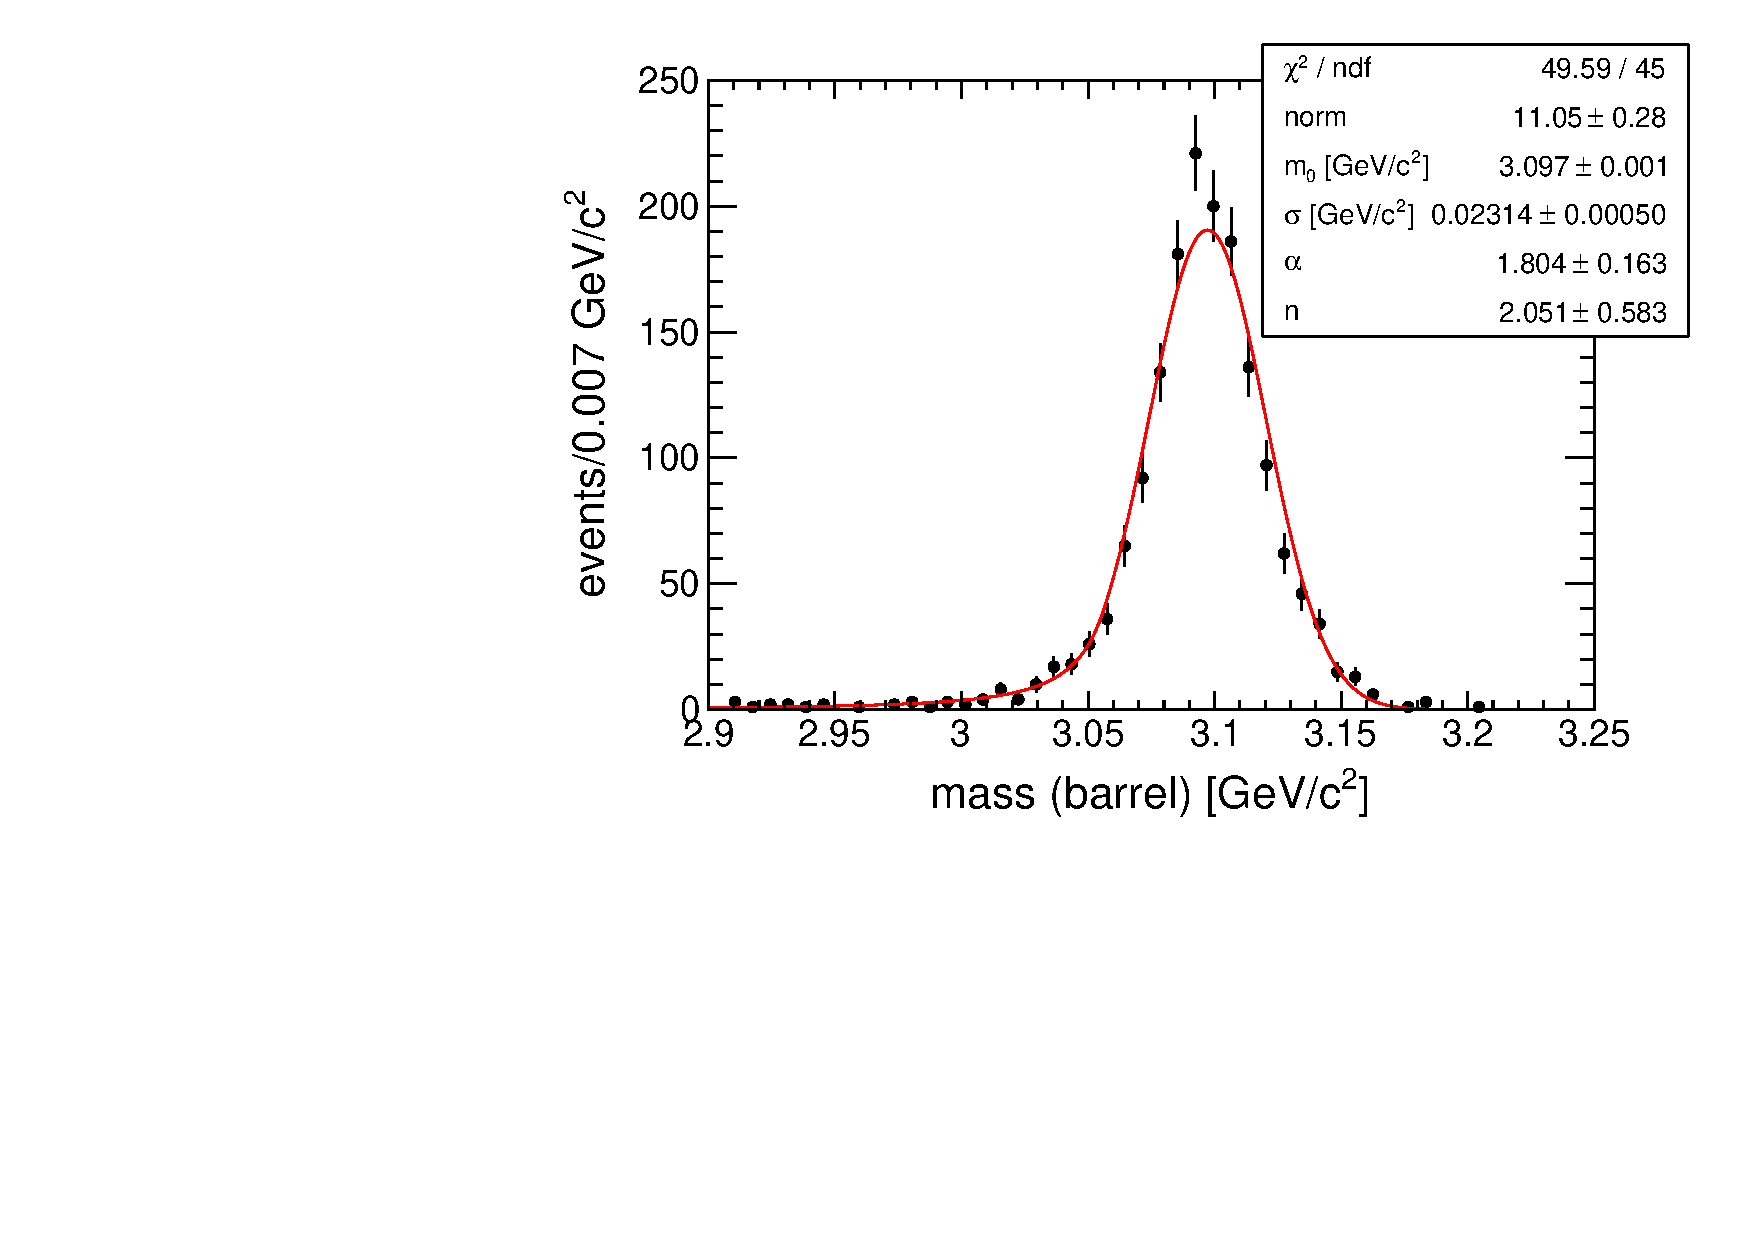
\includegraphics[width=0.48\linewidth]{PLOTS/jpsi_peak_mc.pdf}
\end{tabular}
\caption{Fit of the $J/\psi$ resonance mass peak using simulation to extract parameters $\alpha$ and $n$ for the Crystal Ball shape and their correlation. There is a strong negative corelation ($k=-0.9$) between the two parameters, which was incorporated into the final fits of data. \label{fig:respeak_fits_mc}}
\end{figure}

We assume that the background is a linear function of mass, $p_0 + p_1 m$, and use a Crystal Ball shape to fit the shape of the resonances: 
\begin{multline}
CB(m; m_0, \sigma, \alpha, n) = \\ \dfrac{1}{\sqrt{2\pi}\, \sigma} \left\{ \begin{array}{c l} \exp\left(-\dfrac{(m - m_0)^2}{2 \sigma^2}\right) & \mbox{if $(m - m_0)/\sigma > -\alpha$} \\
\exp\left(-\dfrac{\alpha^2}{2}\right)\left[\dfrac{n}{n - \alpha^2 - |\alpha|(m-m_0)/\sigma}\right]^n & \mbox{otherwise} \end{array} \right.
\end{multline}
The peak of the mass distribution (true mass of the particle in this
parameterization) is $m_0$ (GeV/$c^2$), with core resolution $\sigma$
(GeV/$c^2$).  The Crystal Ball parameter $\alpha$ indicates where the
core Gaussian smoothly connects to a low-side $1/(m-m_0)^n$ tail (in
number of standard deviations below the peak).  In the $\omega$ fit,
the $\rho$ is included with mass and width fixed to its PDG values and
allowed to float in normalization, as an additional background.  Each
resonance is fitted in the barrel and endcap separately, with large
differences in $\sigma$ observed between the two regions.  Only in the
$J/\psi$ barrel fit is the Crystal Ball $\alpha$ parameter allowed to
float (in the other seven fits, the value is fixed to the result from
barrel $J/\psi$.)

To better understand the parameters of the Crystal Ball shape suitable for our analysis, we performed
the same fit using simulated $J/\psi$ events, see results shown in Fig.~\ref{fig:respeak_fits_mc}. It
was found that there is a strong negative correlation between the parameters $\alpha$ and $n$, which
determine the tail behavior of the function. The correlation coefficient was found to be $k=-0.9$. While
this has negligible effect on the acceptance (the signal corridor is defined to be $5\sigma$ in core resolution,
while variations in $\alpha$ and $n$ mainly modify the shape near $\sigma \sim 2$--$3$) and is consistent with the
measurements in data, we incorporated this correlation into the fit and used simulation prescribed parameters
for $\alpha$ and $n$.

Results of the fits are shown in Fig.~\ref{fig:respeak_fits} overlaid
on the data. Parameters of the fitted function were compared to the
simulation predictions and were found to be in good agreement as shown
in the main text (Fig.~\ref{fig:resolution}). Because mass resolutions
depend on the mass, the shape of the dependency was taken from the
simulation. In addition, as shown in the main text, mass resolutions
weakly depend on the momentum (boost) of the dimuon system and we used
simulation to determine the spread in the fit parameters using a broad
range of dimuon momenta. Because the spread is small and has little
effect on the final results, we use it as a measure of the systematic
uncertainties in parameterizing the signal shape.

\section{Background Composition of the Low Mass Dimuon Sample}
\label{sec:analysis_of_the_low_mass_background_composition}

To understand the composition of the dimuon events with low invariant mass of muon pairs, we
first separate the sample into two orthogonal sub-samples: one enriched with the dimuons from
the $b\bar{b}$ production and the other depleted of the $b\bar{b}$ events. This is achieved 
using selections based on isolation of the muon pair and the flight distance calculated using the 
common vertex of the two muons. We then compare events in data with the predictions based
on simulated events for each of the main backgrounds: $b\bar{b}$ production, light flavor QCD
multi-jet production, prompt resonance production (e.g. $J/\psi$) and Drell-Yan 
($pp \to \gamma^* \to \mu \mu$ using Pythia 8 with no explicit low mass cut-off, although Pythia
cuts it at $\sqrt{q^2_{\gamma^*}} \sim 0.35$~GeV/c$^2$). 

The isolation variable is defined using tracks around the dimuon system excluding both of the 
muons used in constructing the dimuon candidate such that the two close-by muons do not 
veto one another:
\begin{equation}
Iso = \sum_{\mbox{\scriptsize tracks}} p_T \mbox{ if } p_T > 1.5\mbox{ GeV/$c$, }
\Delta R < 0.4 \mbox{, and not a muon,}
\end{equation}
where the $p_T$ threshold and $\Delta R$ radius were chosen to minimize sensitivity to
tracks from the pile-up and to achieve a near flat distribution of the isolation distribution
for dimuons from the $b-$jets near $Iso = 0$ (using a simulated sample of $b\bar{b}$ MC events). 

The flight distance is defined as
\begin{equation}
L_{xy} = \frac{(v_x - V_x) p_x + (v_y - V_y) p_y}{\sqrt{{p_x}^2 + {p_y}^2}}
\end{equation}
where ($v_x$, $v_y$) is the 2-D position of the dimuon vertex, ($p_x$,
$p_y$) is the 2-D projection of the dimuon momentum vector, and
($V_x$, $V_y$) is the 2-D position of the closest primary vertex in
the $z$ direction ($z$ is parallel with the beamline).

Distributions for both variables, $Iso$ and $L_{xy},$ are shown in Fig.~\ref{fig:support_iso_lxy}, for
the whole mass distribution $m_{\mu\mu}<5$ GeV/c$^2$, and also for two subsets of the events. The 
first subset is events from the ``continuum'' ($1.1 < m_{\mu\mu} < 2.9$~GeV/$c^2$) part of the
spectrum, and the second one contains events from the``low-mass'' part of the spectrum
($0.35 < m_{\mu\mu} < 0.5$~GeV/$c^2$). Note that the ``low mass'' region does not include the
very low mass region of $0.25 < m_{\mu\mu} < 0.35$~GeV/$c^2$. The ``continuum'' and 
``low-mass'' ranges are motivated by different composition of the backgrounds as shown in 
Fig.~\ref{fig:support_mass}(a), where these ranges are indicated by dotted vertical lines. 
As expected, Drell-Yan and prompt resonances are well isolated, while $b\bar{b}$ is not. The 
$L_{xy}$ variable provides another handle on separate the long living and prompt sources of background. 
Drell-Yan and prompt resonances form a peak centered on $L_{xy} = 0$, while $b\bar{b}$ has a 
long tail toward positive $L_{xy}$ due to the long lifetimes of $B$ hadrons. Note 
that vertices with negative $L_{xy}$ are mis-measured; this provides a direct indication of the vertex
resolution.  Vertex resolution degrades when the opening angle becomes small (or equiavlently the low 
invariant mass $m_{\mu\mu}$, particularly as it approaches the kinematic threshold of 
$m_{\mu\mu}=2 m_\mu$), which is why the symmetric peak in the low-mass bin is wider than in all other bins.

\begin{figure}
\centering
\begin{tabular}{ccc}
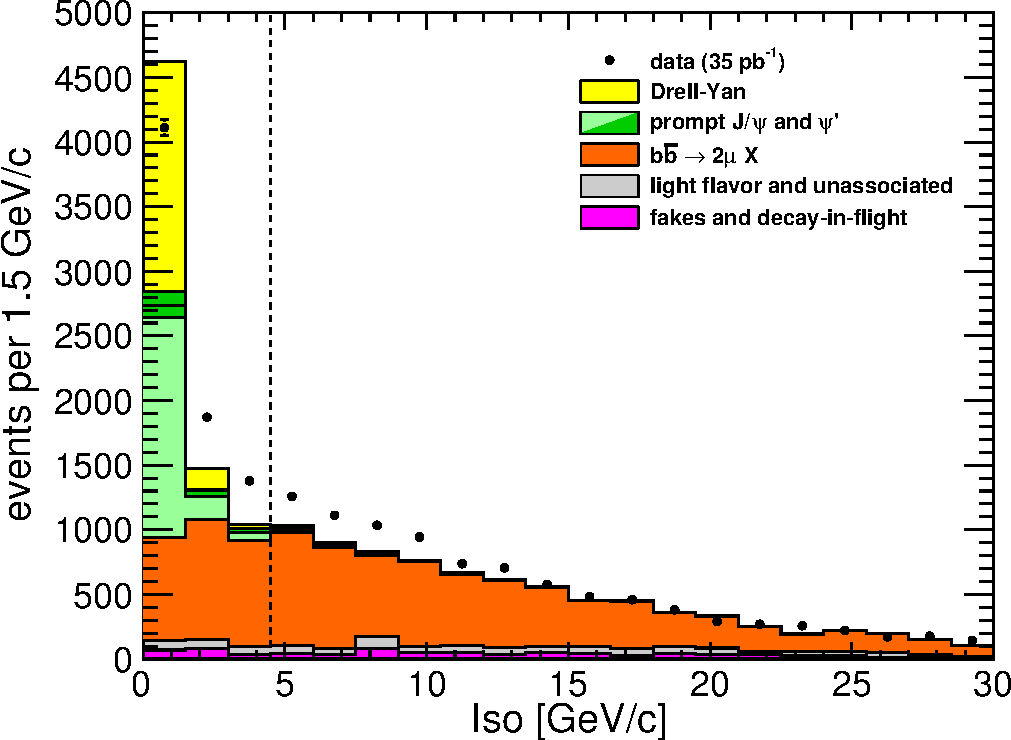
\includegraphics[width=0.3\linewidth]{PLOTS/support_iso_all.pdf} &
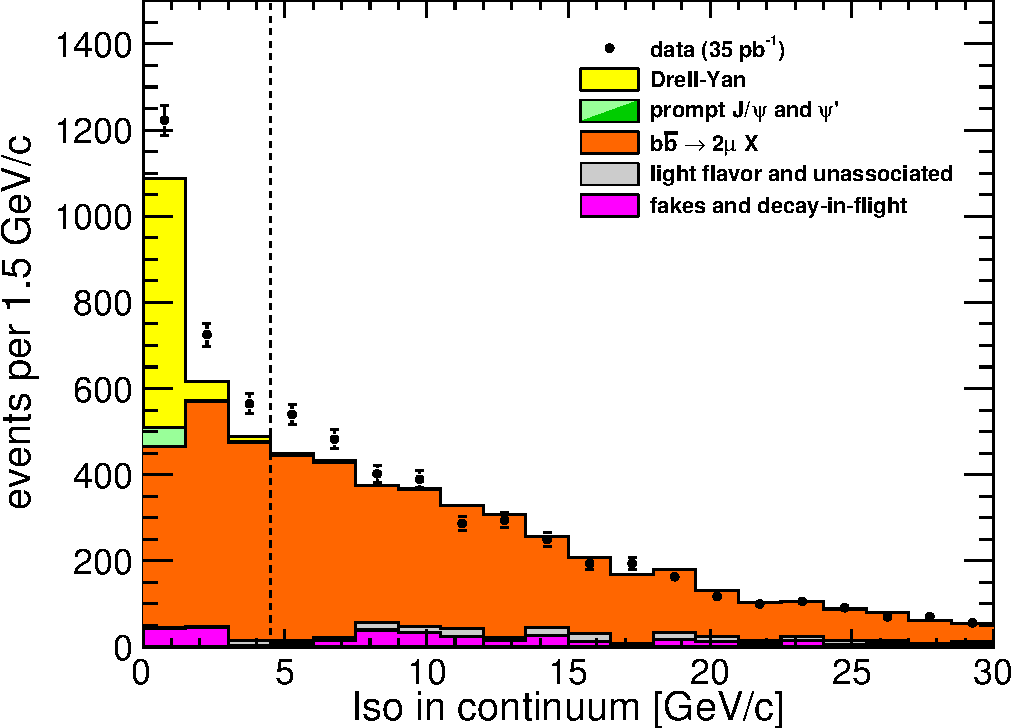
\includegraphics[width=0.3\linewidth]{PLOTS/support_iso_continuum.pdf} &
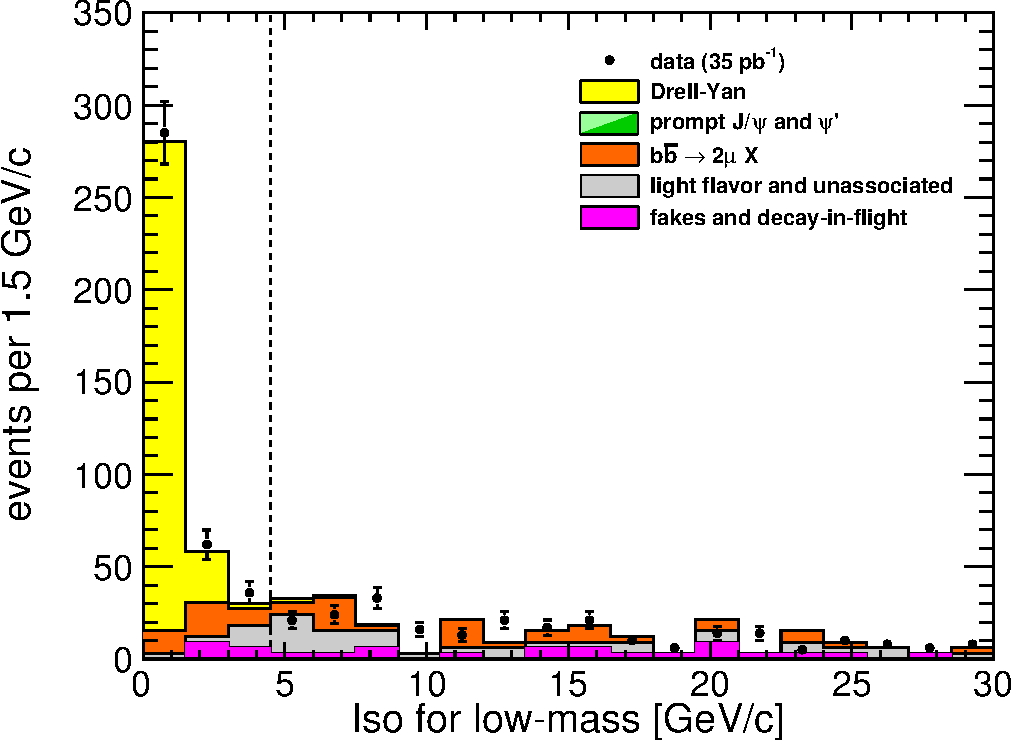
\includegraphics[width=0.3\linewidth]{PLOTS/support_iso_lowmass.pdf} \\
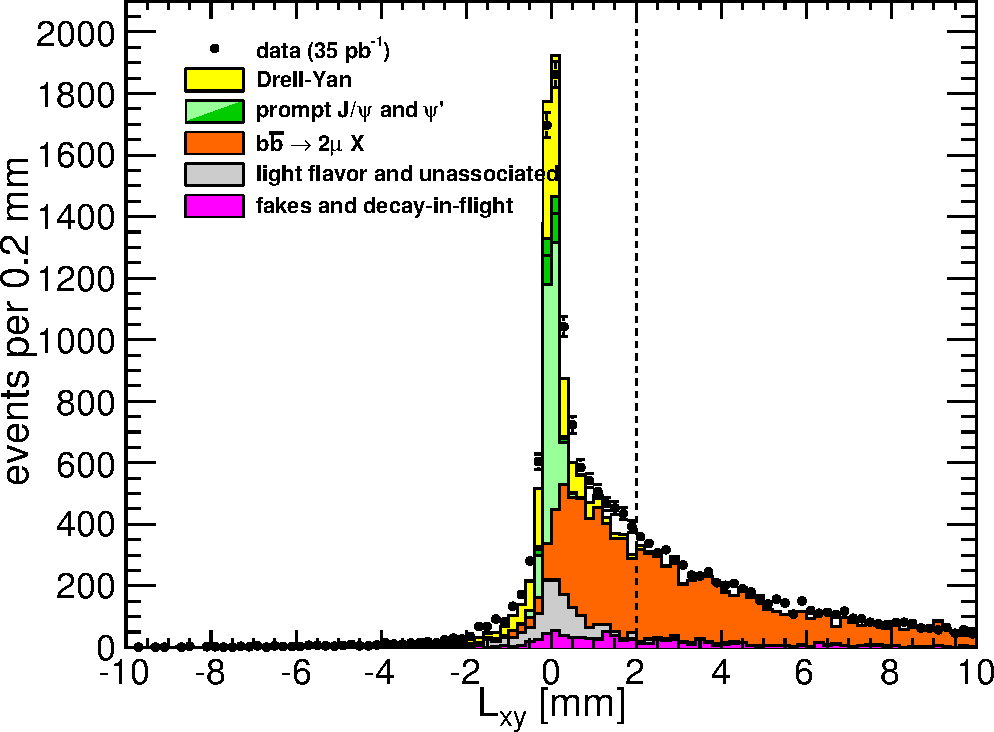
\includegraphics[width=0.3\linewidth]{PLOTS/support_lxy_all.pdf} &
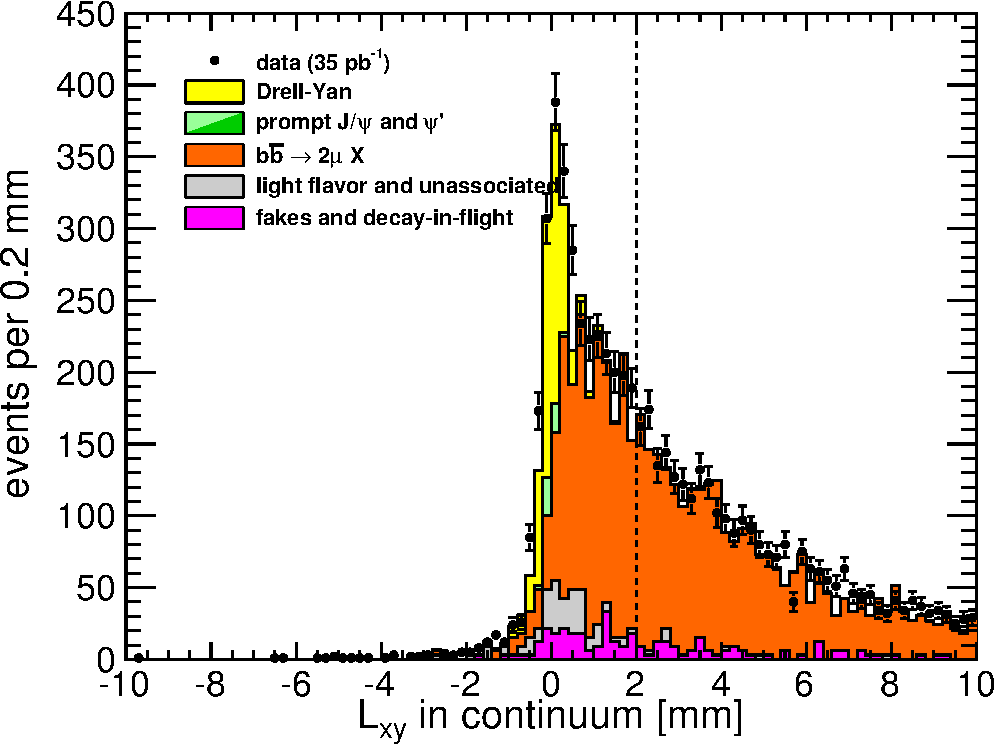
\includegraphics[width=0.3\linewidth]{PLOTS/support_lxy_continuum.pdf} &
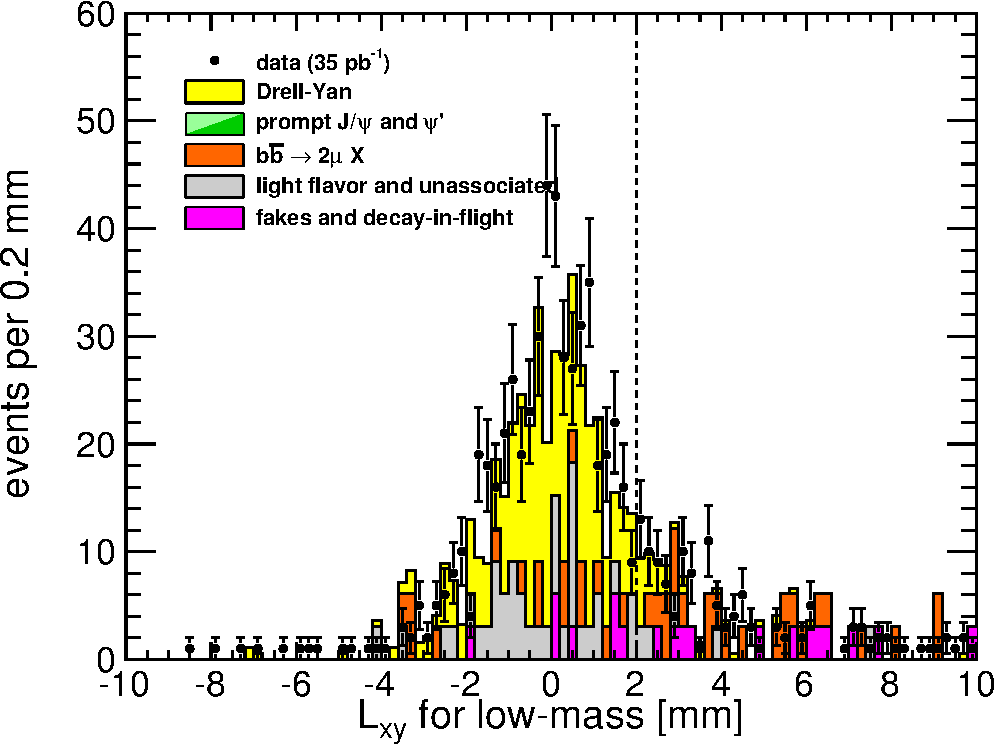
\includegraphics[width=0.3\linewidth]{PLOTS/support_lxy_lowmass.pdf} \\
\end{tabular}
\caption{(a): Track-based isolation (see text for definition) for the whole sample. (b) The same distribution for events with $m_{\mu\mu}=1.1-2.9$~GeV/$c^2$ (the continuum), and (c): for the low mass region $m_{\mu\mu}=0.35-0.5$~GeV/$c^2$. (d): Distance of the dimuon vertex (in $x$-$y$) from the closest
  primary vertex (in $z$), along the direction of the dimuon momentum
  axis, for the whole sample, (e) distribution for events with
  $m_{\mu\mu}=1.1-2.9$~GeV/$c^2$. (f): for the low mass region
  $m_{\mu\mu}=0.35-0.5$~GeV/$c^2$. Note that the events in the ``very
  low mass'' range  $0.25 < m_{\mu\mu} < 0.35$~GeV/$c^2$ are not
  included in the low-mass or continuum plots. \label{fig:support_iso_lxy}}
\end{figure}

These observations prompted us to partition the data into two regions dominated by $b\bar{b}$ and prompt/Drell-Yan, respectively (each containing resonance and continuum contributions) using the ``$b\bar{b}$ cuts'' already mentioned in Eqn.~\ref{eqn:bbcuts} of the main text:
\begin{equation}
Iso > 4.5\mbox{ GeV/$c$ {\bf or }} L_{xy} > \mbox{2 mm.}
\end{equation}
The ranges are indicated with dotted vertical lines in
Fig.~\ref{fig:support_iso_lxy}. Our conclusion is that the data is
reasonably well described by the simulation (with the exception of some of the resonances neglected during event generation) and the two agree well for $m_{\mu\mu}>0.35$ GeV/c$^2$ with no unexpected backgrounds or other features. Small differences between the data and simulation, e.g.\ in the shape of isolation distributions are not a concern as we never use these cuts in the main analysis selections. Also, the agreement in isolation distributions is likely affected by the lack of simulated $b\bar{b}$ events with lower $\hat{p}_T$ (the sample used in these comparisons was generated using $\hat{p}_T > 30$ GeV/c).

In addition to background composition studies, another use of the selections based on isolation and flight distance is to demonstrate the approximate scaling of the dimuon invariant mass distribution in $b\bar{b}$ events with the dimuon transverse momentum (see Fig.~\ref{fig:support_bbbarcut_limits} in the main text). This assumption is used in constructing the dimuon invariant mass template for background events in region (a-1) and for the triggered dimuon template for background events in region (b-1).  It is therefore important to verify that these selections do not bias the shape of the dimuon mass spectrum for $b\bar{b}$ events. Fig.~\ref{fig:support_bbbarcut_efficiency} shows the efficiency of the $b\bar{b}$ cut versus dimuon invariant mass using simulated $b\bar{b}$ events. The efficiency is uniform at the level of precision required for the templates affirming the validity of our assumptions\footnote{Note that the use of both $L_{xy}$ and $Iso$ variables leads to a more uniform efficiency as compared to the case of using isolation only, although the bias in the latter case is not too large.}

\begin{figure}
\begin{center}
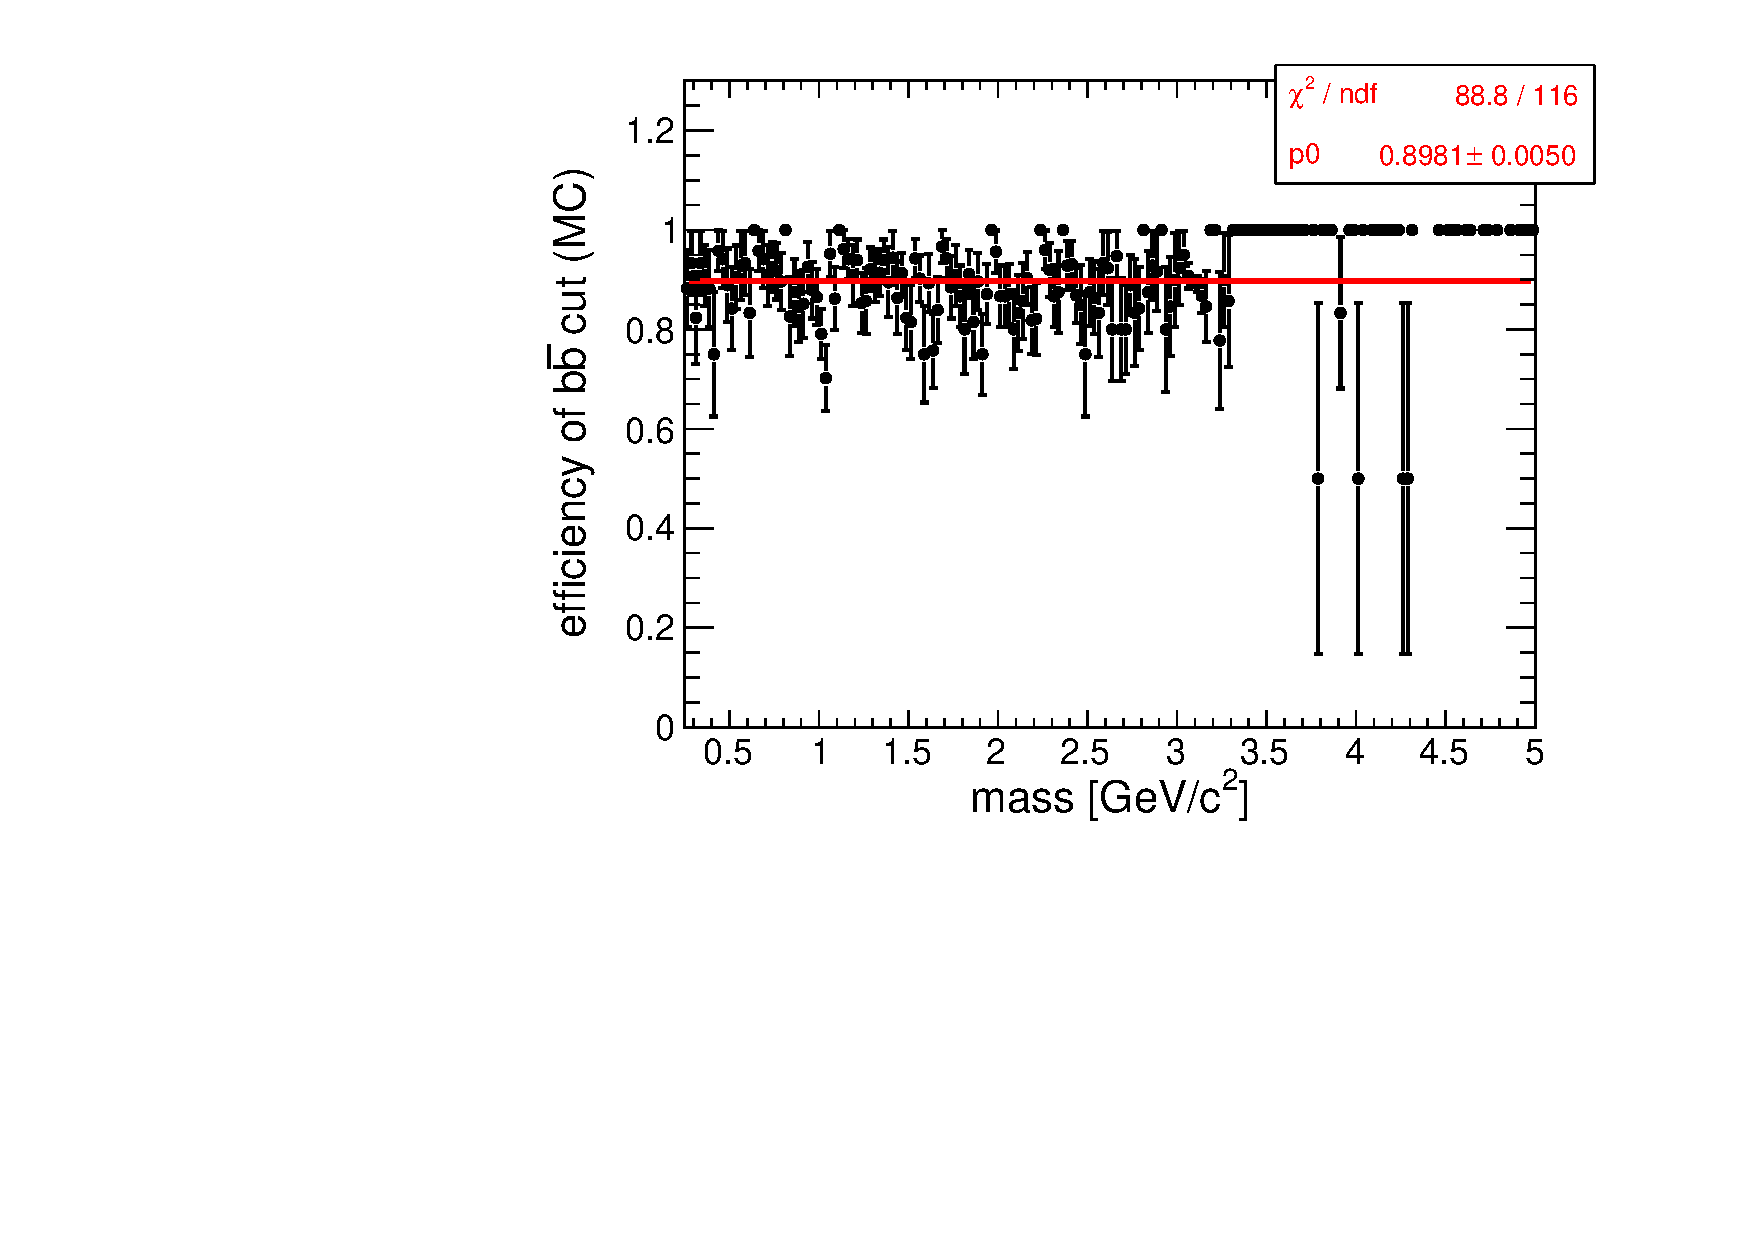
\includegraphics[width=0.6\linewidth]{PLOTS/support_bbbarcut_efficiency.pdf}
\end{center}
\caption{Efficiency of the $b\bar{b}$ cut for simulated $b\bar{b}$
  events, demonstrating that the efficiency is constant, so the
  $b\bar{b}$ cuts do not introduce a shape bias. \label{fig:support_bbbarcut_efficiency}}
\end{figure}

\subsection{The Very Low Mass Region $m_{\mu \mu} < 0.35$ GeV/c$^2$}

In this section we discuss the properties of the events comprising the very low mass excess not predicted by the simulated SM background processes used in this analysis. The excess has a shape of a low-mass rise towards the lower edge of the invariant mass distribution. The excess is very significant in the ``very low mass'' range  $0.25 < m_{\mu\mu} < 0.35$~GeV/$c^2$ and the tail of it may be still present all the way up to $m_{\mu\mu} \sim 0.55$ GeV/c$^2$. 

The shape of the ``excess'' is clearly not consistent with a dimuon resonance as could be concluded from our studies of signal shapes (Sec.~\ref{sec:signal_mass_spectrum_shape} and \ref{sec:appendix_signal_shape_studies}) that extend to very low masses, which indicate that a resonance will have a very narrow shape. In our nominclature, the excess is only present in the ``$b\bar{b}$-enhanced'' region while in the ``$b\bar{b}$ -depleted'' sample a similar rise is consistent with being the low mass DY events and the residual excess below $m_{\mu\mu}=0.35$~GeV/$c^2$ is a likely artifact of the default low mass $\sqrt{q^2} \sim 0.35$ GeV/$c^2$ cut-off in the Pythia 8 Drell-Yan generation. However, at such low invariant masses our definition of the $b\bar{b}$ enriched samples becomes not fully appropriate as the $L_{xy}$ resolution becomes very poor for boosted dimuons as the two muon tracks are nearly parallel. One can see that effect by comparing  Figs.~\ref{fig:support_iso_lxy}(d) and (f), showing the $L_{xy}$ resolution for simulated DY events in continuum and for the mass range $0.25 < m_{\mu\mu} < 0.35$~GeV/$c^2$. For lower masses, the $L_{xy}$ resolution quickly deteriorates becoming very broad. As a result, our ``$b\bar{b}$ cuts'' continue being appropriate for selecting an enriched sample of $b\bar{b}$ events, but no longer constraints the DY events to the $b\bar{b}$-depleted sample as the requirement of $L_{xy}>2$~mm divides DY events in almost equal fractions between the ``$b\bar{b}$-enriched'' and the ``$b\bar{b}$-depleted'' subsets. Therefore, to study the very low mass excess, we partition the sample into $b\bar{b}$-enriched and DY-enriched samples using isolation only, $Iso<4.5$ GeV/c for the DY-enriched and $Iso\ge 4.5$ GeV/c for the $b\bar{b}$-enriched subsamples.The distributions of invariant mass of the dimuon system for the two subsampes is shown in Figs.~\ref{fig:support_very_low_mass}(a) and (b). It is very evident now that the bulk of the excess is due to the unsimulated DY events at very low $Q^2$. Although there is a residual excess in the non-isolated subsample, which we are still studying, this unknown background component is absolutely inconsistent with signal due to its broad shape and constitutes less than 20\% of all backgrounds in that region making it  have no effect on the analysis results. Figures.~\ref{fig:support_very_low_mass}(c) and (d) show the $L_{xy}$ distribution for the very low mass events in isolated and non-isolated subsets reaffirming our earlier observations about degradation of the $L_{xy}$ resolution at very low masses (note that the units on $x-$axis being cm and not mm as in other $L_{xy}$ plots). It also shows that the residual background events in the non-isolated sample are prompt and very similar to DY events in the isolated samples in terms of $L_{xy}$ distribution. 

We therefore conclude that the bulk of the ``excess'' in the very low mass region is understood and is due to Drell-Yan events with very low $Q^2(\gamma^*)$ not generated in our DY simulated samples. The remaining excess is DY-like (except it appears to be not isolated, which perhaps could indicate either an off-shell photon production in jets or a tracking reconstruction artefact in the environment of two very close tracks) and is small compared to the overall size of the background in that region (less than 20\%), which is well within the margin of our systematic uncertainties.

\begin{figure}
\centering
\begin{tabular}{cc}
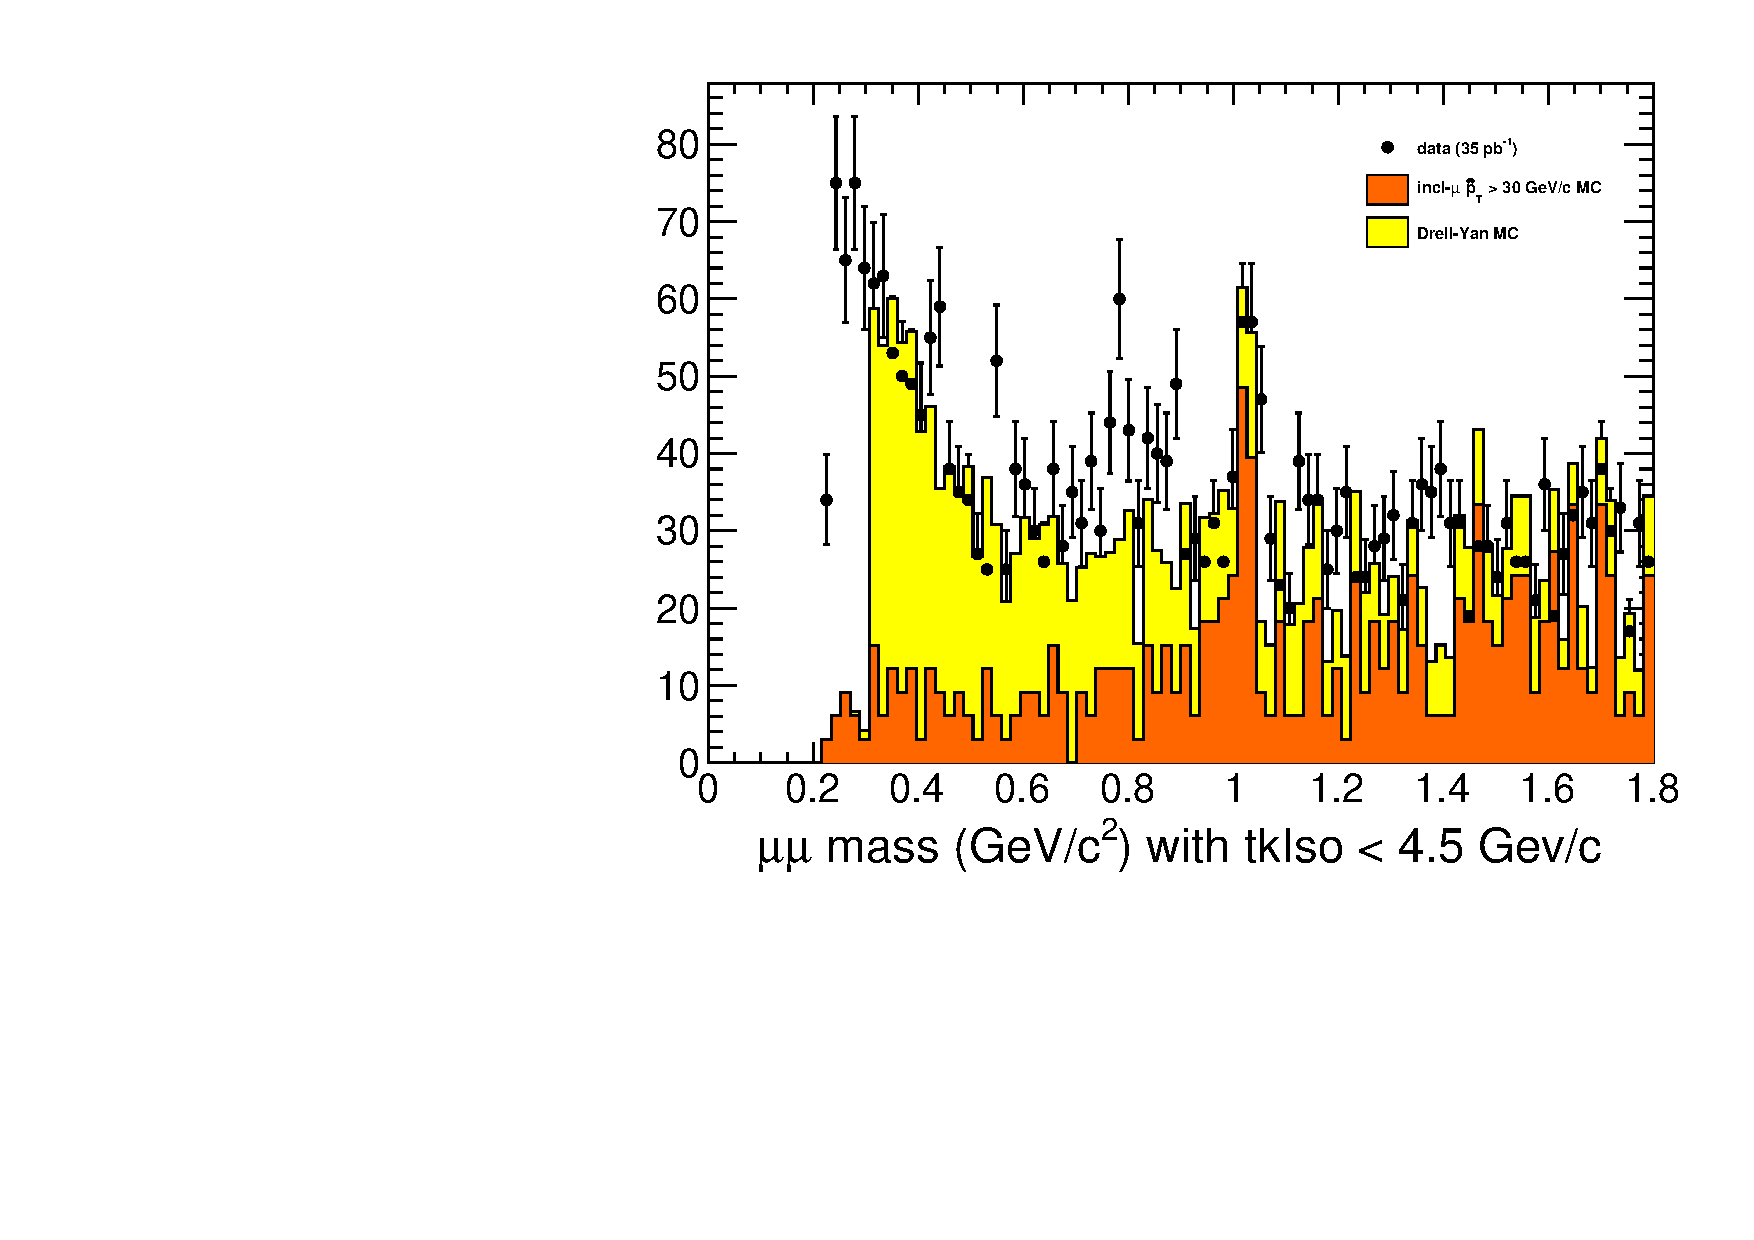
\includegraphics[width=0.45\linewidth]{PLOTS/02_mass_iso_less_45.pdf} &
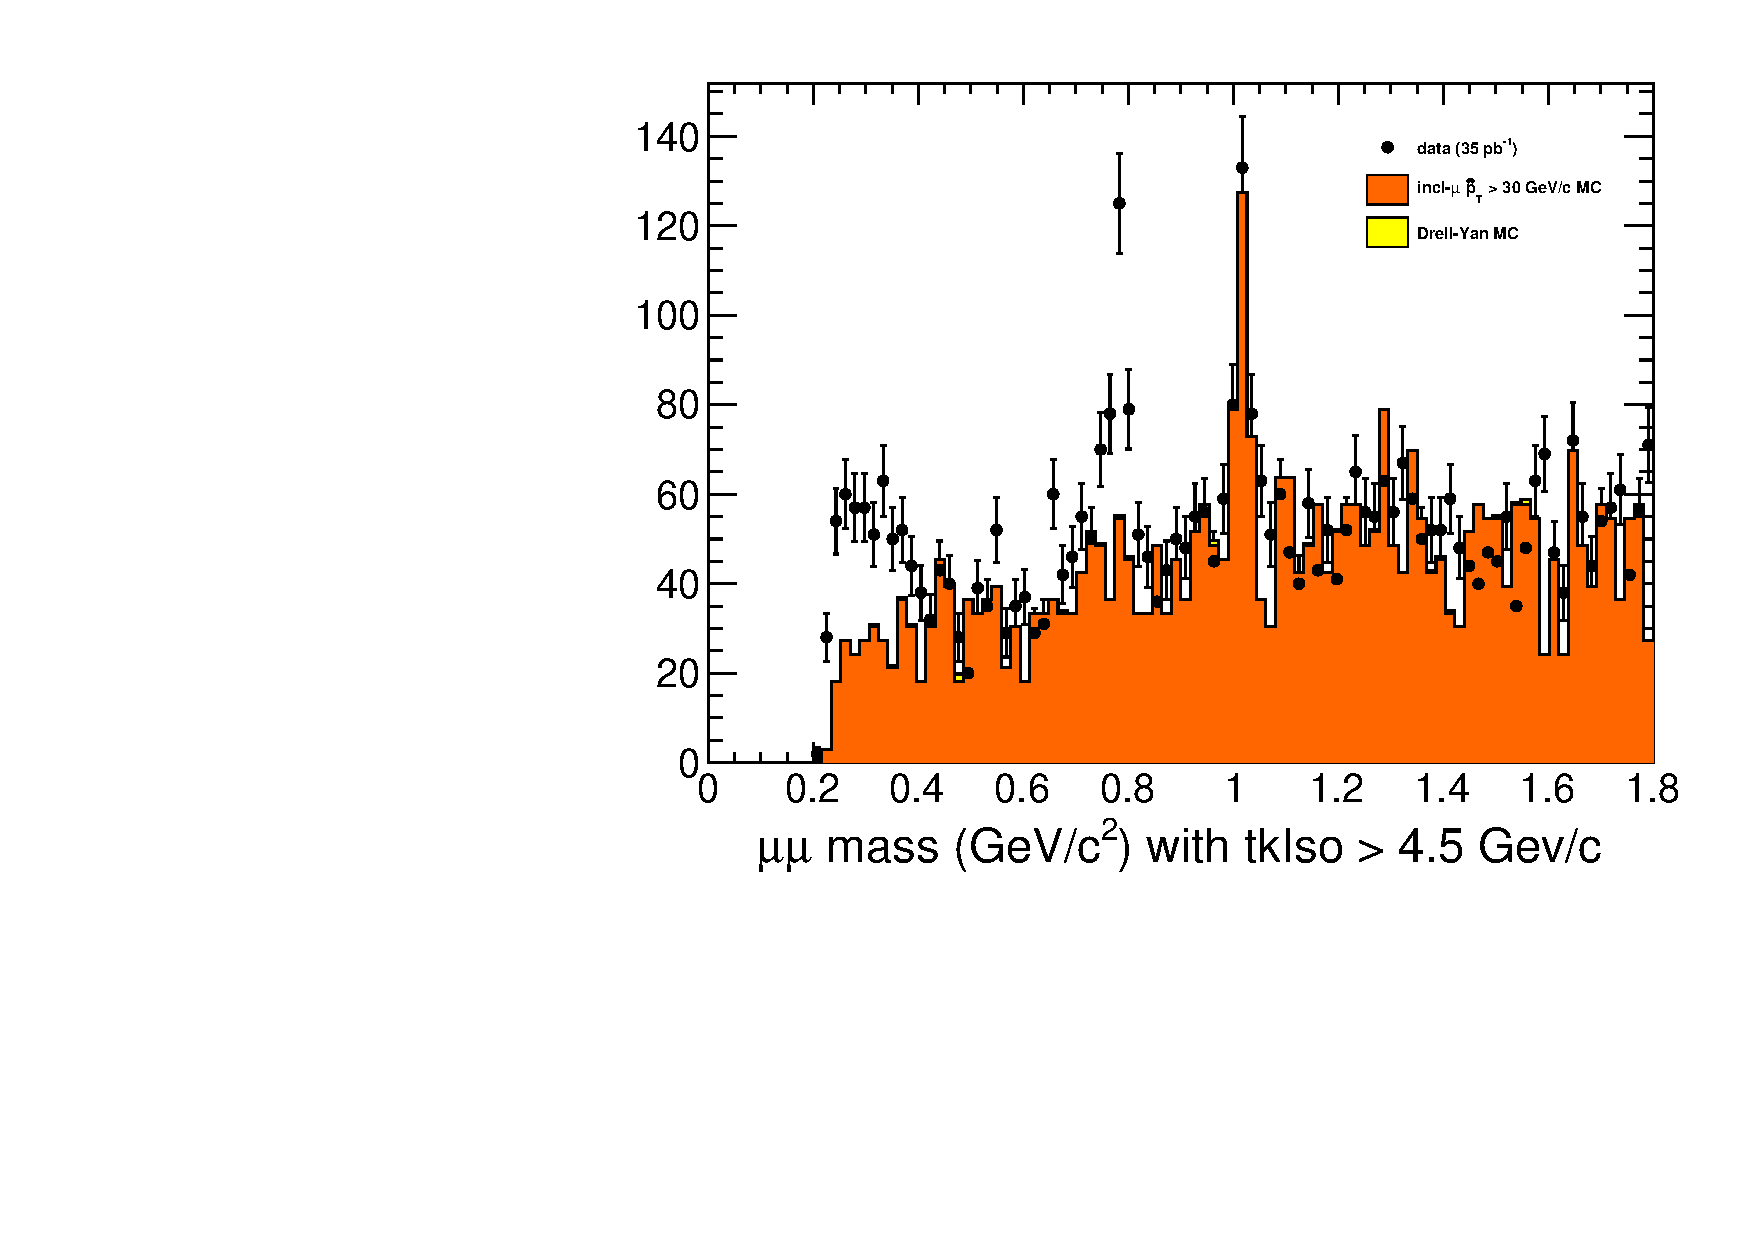
\includegraphics[width=0.45\linewidth]{PLOTS/01_mass_iso_more_45.pdf} \\
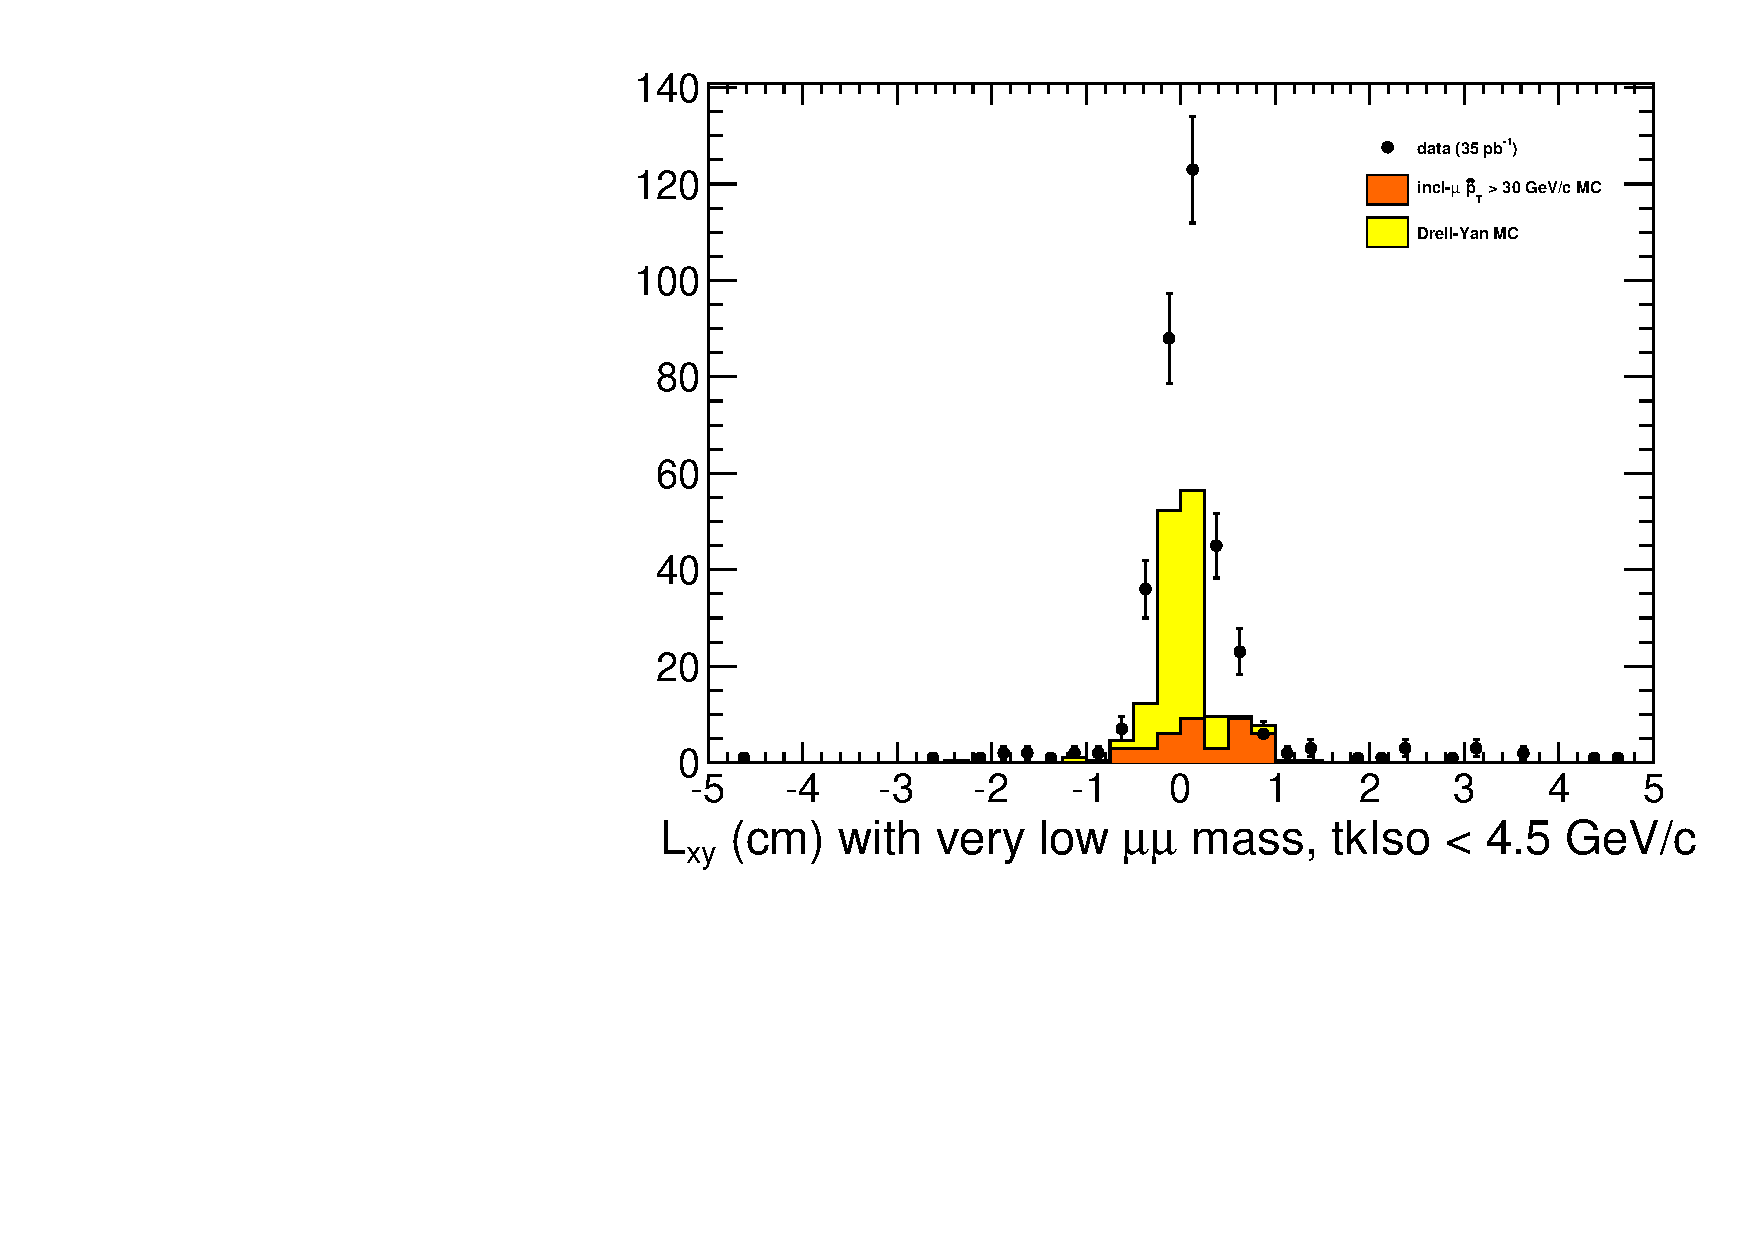
\includegraphics[width=0.45\linewidth]{PLOTS/05_lxy_iso_less_45.pdf} &
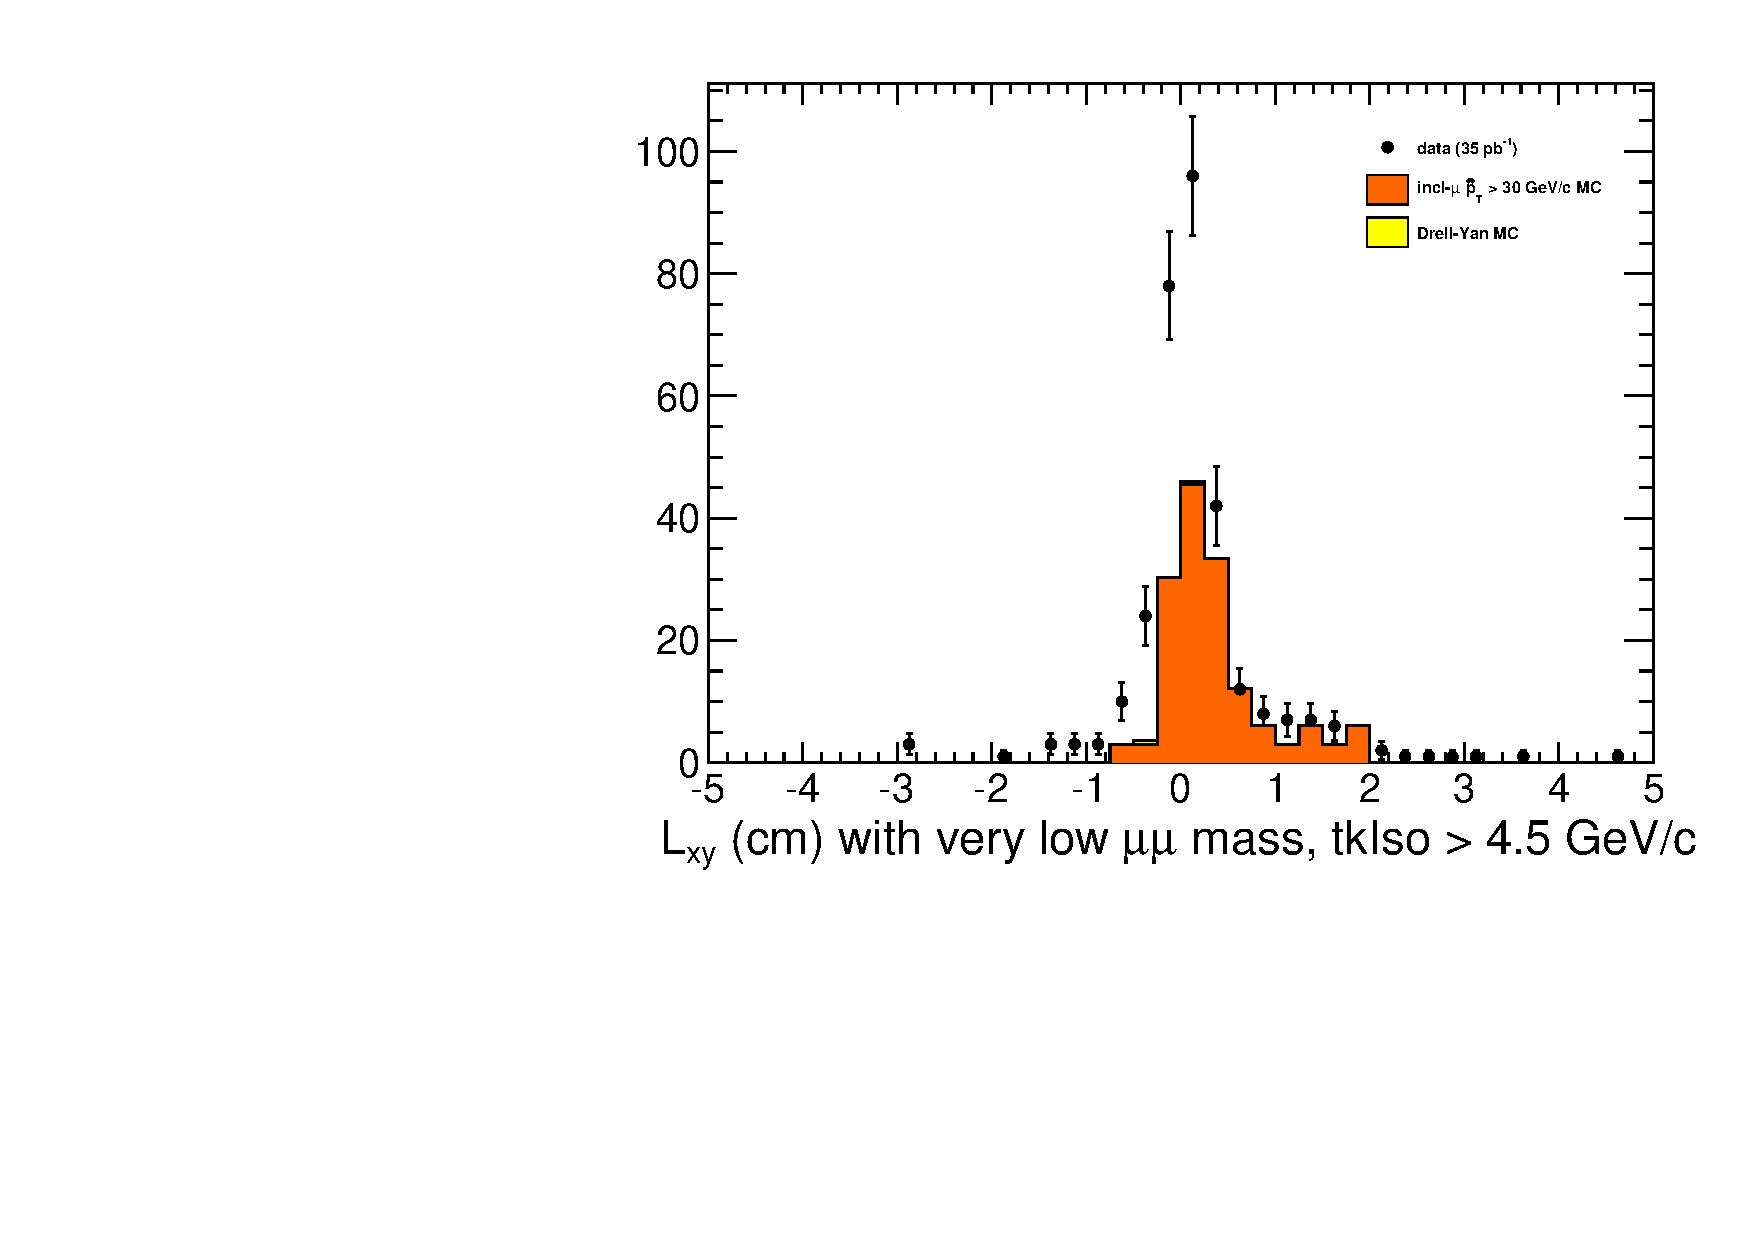
\includegraphics[width=0.45\linewidth]{PLOTS/04_lxy_iso_more_45.pdf} \\
\end{tabular}
\caption{(a): Invariant mass distribution for events with $Iso<4.5$ GeV/c. (b): The same distribution for $Iso \ge 4.5$ GeV/c. (c): $L_{xy}$ distribution for isolated ($Iso<4.5$ GeV/c) events in the very low mass region $0.25<m_{\mu\mu}<0.35$ GeV/c$^2$. (d): $L_{xy}$ distribution for non-isolated events in the very low mass region. \label{fig:support_very_low_mass}}
\end{figure}

\section{Supporting plots for background mass templates}

\subsection{Dimuon Mass Spectrum for Misidentified Muons in Simulation}
\label{sec:appendix_mc_decayinflight_fakes}

Dimuon invariant mass templates for background events in regions (a-2) and (a-3),
containing high multiplicity mu-jets, has a component where a dimuon candidate 
originates from hadronic tracks that are misidentified as muons.  While we measure
the actual invariant mass distribution for pairs of misidentified muons directly 
from the data (see Sec.~\ref{sec:background_spectrum_for_a_2}), it is nevertheless
interesting to compare data driven results with the simulation predictions. The source 
of misidentified muons has two main components: a  $\pi^\pm$, $K^\pm$, or (more rarely) 
strange baryon decays within the detector, and due to accidental matches of tracks with hits 
in the muon chambers. We use the simulated muon enriched QCD multi-jet sample to
constuct dimuon candidates using reconstruction level information. We then select dimuon
candidates reconstructed from misidentified muons from each of these two categories.  For
the first category (decays in flight), we identify reconstructed muons matched to a generator-level muon 
whose parent is a long-lived hadron to select misidentified muons. For the second category, we 
identifying reconstructed muon candidates with no generator-level match. 
Figure~\ref{fig:mc_mass_spectra_fakes} shows the invariant mass spectra for dimuon 
candidates constructed using misidentified muons of each type. Evidently, the spectra are 
very similar to one another, and also similar to the mass templates derived from data in Sec.~\ref{sec:background_spectrum_for_a_2} reaffirming validity of our background modeling procedure.

\begin{figure}
\begin{center}
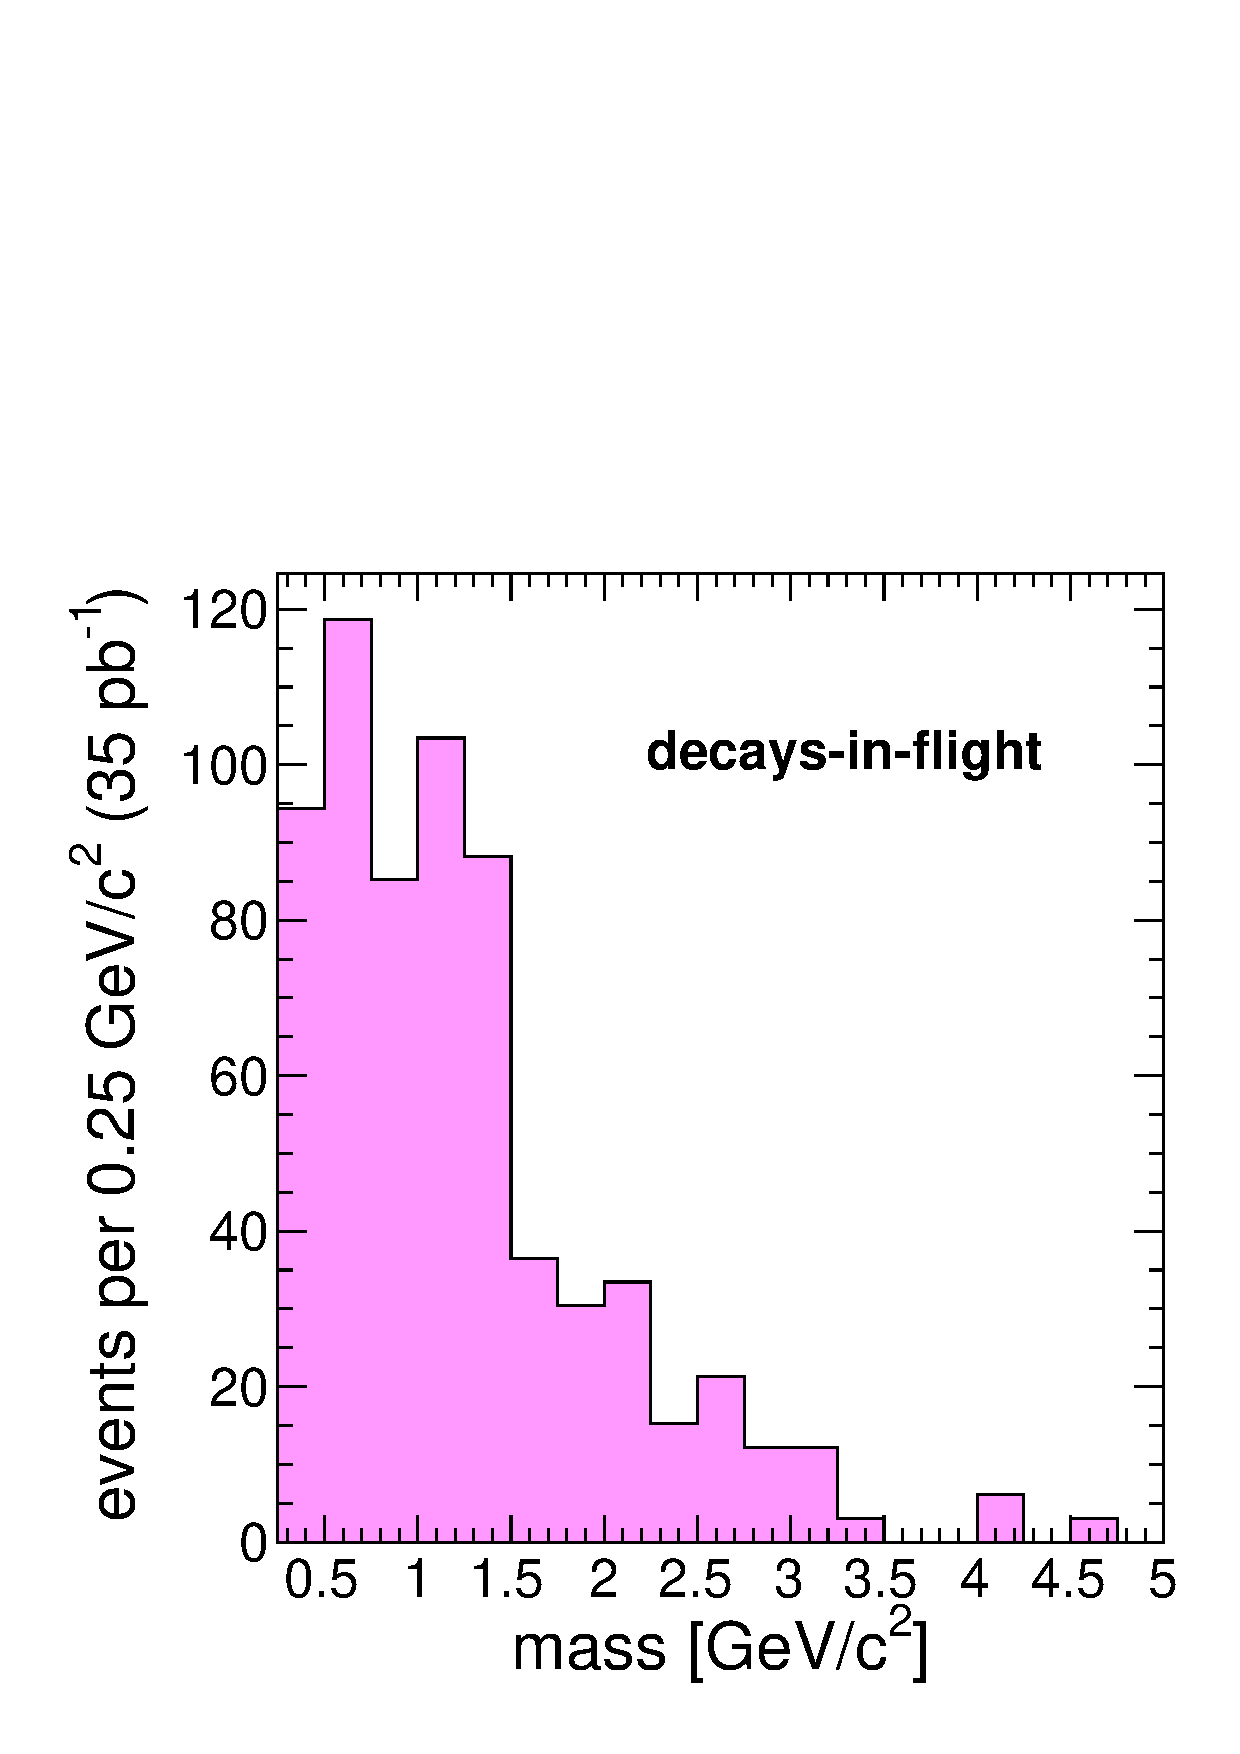
\includegraphics[width=0.3\linewidth]{PLOTS/mc_mass_spectra_onlyinflights.pdf} \hspace{0.25 cm}
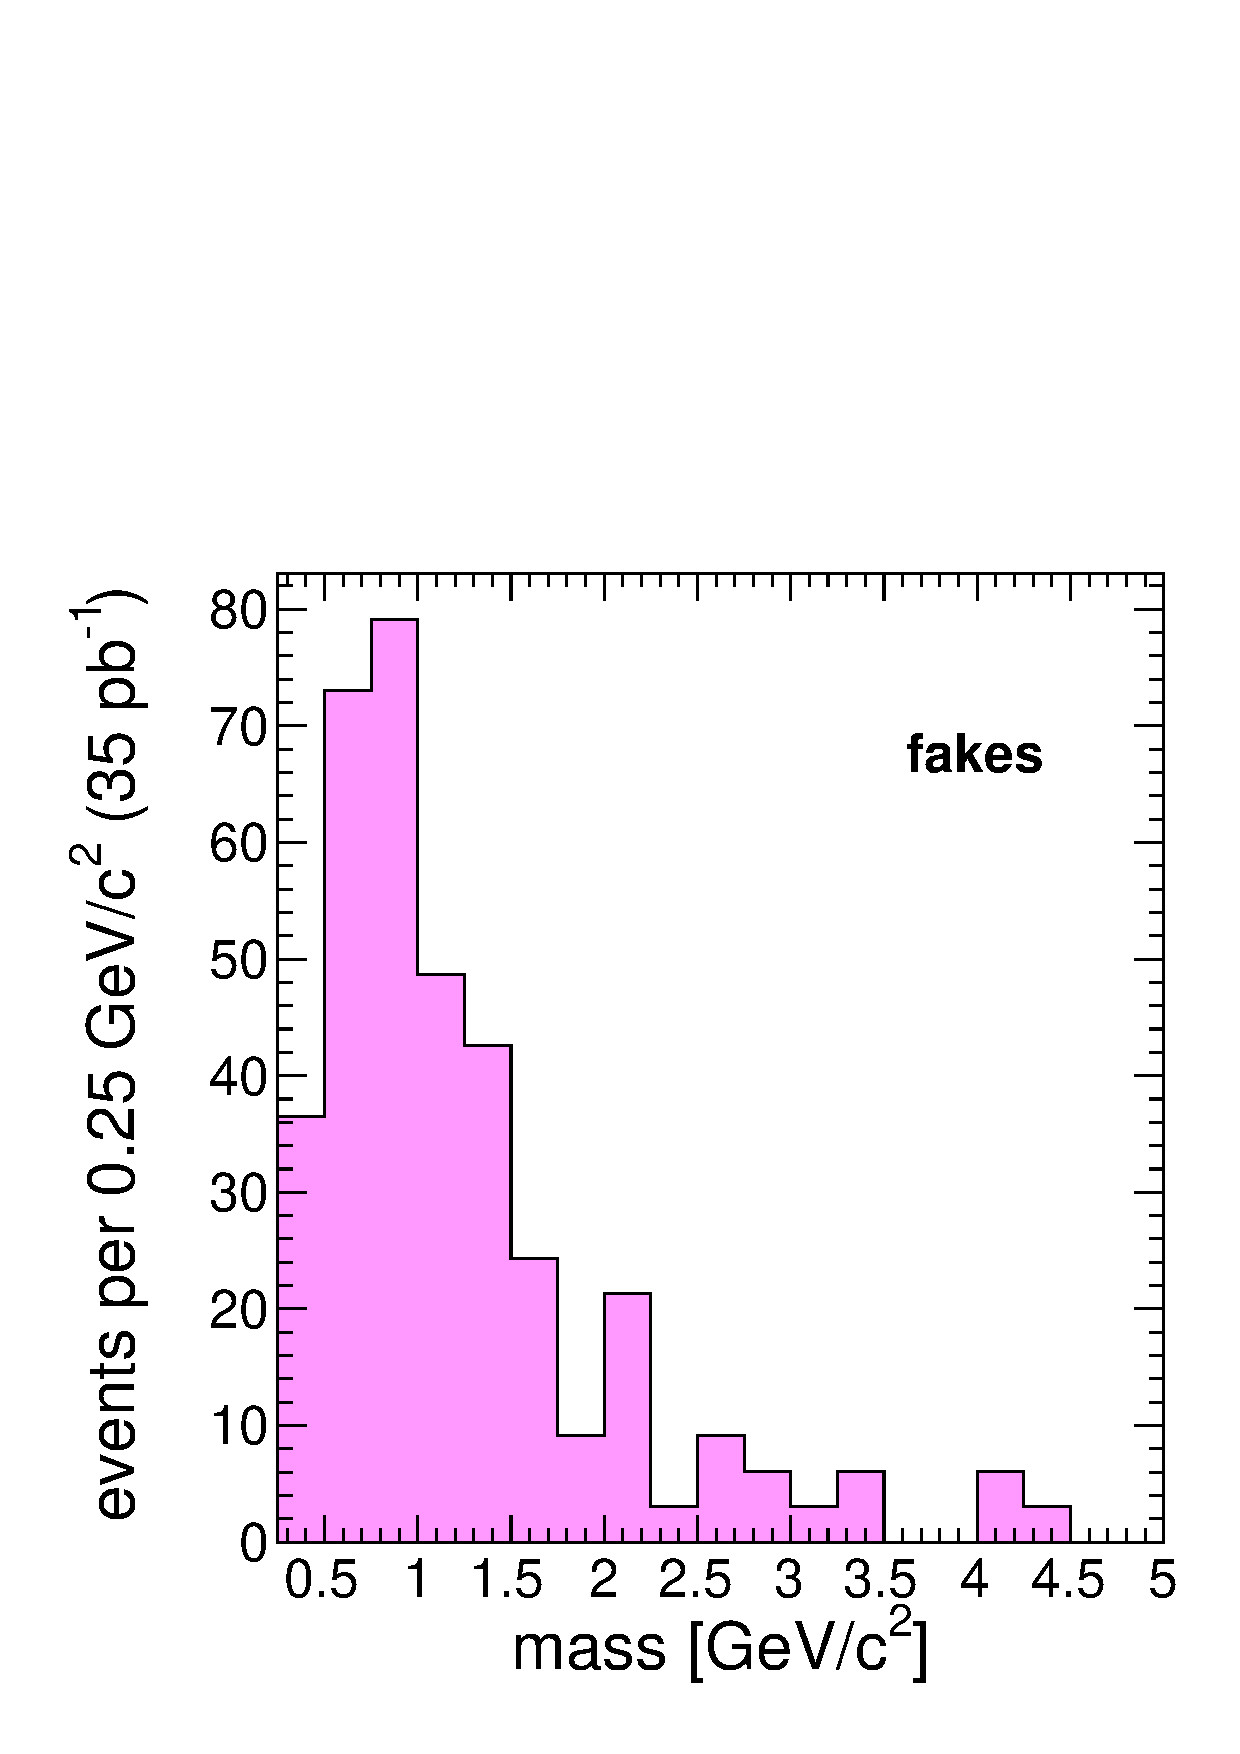
\includegraphics[width=0.3\linewidth]{PLOTS/mc_mass_spectra_onlyfakes.pdf}
\end{center}
\caption{Distributions of dimuon mass for dimuons containing decay-in-flight and
  fake muons in inclusive-muon Monte
  Carlo. \label{fig:mc_mass_spectra_fakes}}
\end{figure}

\subsection{Weighting procedure for triggered and other dimuons (b-1)}
\label{sec:appendix_b_1_weighting}

In events with two well-separated dimuons (b-1), at least one of the
two dimuons must contain a trigger muon, which introduces an asymmetry
between the two dimuons with implications for the shape of the mass
spectrum (discussed in Sec.~\ref{sec:background_spectrum_for_b_1}).
Sometimes, however, both dimuons contain a trigger: in that case, we
randomly assign the labels ``triggered'' and ``other.''  While this
has no effect on the shape of the triggered dimuon mass spectrum, the
triggerable part of the other dimuon mass spectrum becomes depleted by
a factor of $\tfrac{1}{2}$.  To produce the correct mass templates, we
make the same correction in the background-enriched samples used to
construct the templates: events in the ``other dimuon'' template with
a muon with the right kinematics to satisfy the trigger ($p_T >
5$~GeV/$c$ and $|\eta| < 0.9$) are weighted by $\tfrac{1}{2}$.  Note
that the final analysis fit requires no weighting.

To demonstrate that this weighting procedure produces the correct
templates, we performed two toy Monte Carlos, one with uniform
distributions (to see the bias by eye) and another with more realistic
distributions.  Background-enriched samples and
background-in-signal-region samples were simulated independently, but
with the same distributions as each other.  The uniform toy Monte
Carlo was simulated by throwing random $p_T$ and $\eta$ variables
uniformly in 0--50~GeV/$c$ and $|\eta| < 2.4$, respectively, in three
cases: background-enriched for trigger, background-enriched for other,
and a 2D distribution ($p_{T1}$, $p_{T2}$, $\eta_1$, $\eta_2$) for the
signal region.  The background-enriched for trigger sample was
required to satisfy a simulated trigger ($p_T > 15$~GeV/$c$ and
$|\eta| < 0.9$) while the background-enriched for other was not.  The
background-enriched for other events were weighted by a factor of
$\tfrac{1}{2}$ if they happened to satisfy the trigger, however.  The
signal region simulation was required to satisfy the trigger (($p_{T1}
> 15$~GeV/$c$ and $|\eta_1| < 0.9$) or ($p_{T2} > 15$~GeV/$c$ and
$|\eta_2| < 0.9$)), and the dimuons 1 and 2 were assigned labels
``triggered'' and ``other'' the same way as in data: if only one
dimuon satisfied the trigger, it was labeled ``triggered'' and the
other was labeled ``other,'' but if both satisfied the trigger, then
the labels were randomly assigned.  The left-side plots in each of the
four groups in Fig.~\ref{fig:simulation_pteta} shows
background-enriched samples from the uniform toy MC (red lines)
overlaid on projections of the signal samples (black points) from the
uniform toy MC, adjusted for overall normalization.  Each of the four
groups shows a different variable: triggered $p_T$, triggered $\eta$,
other $p_T$, and other $\eta$.  The trigger cuts are evident in the
triggered samples and the $\tfrac{1}{2}$ weighting factor is evident
in the background-enriched other sample.  It is also easy to see that
this weighting exactly compensates for the bias in the signal from
randomly assigning labels in the cases with two triggered dimuons.

For a more realistic demonstration, the toy Monte Carlo was repeated
with realistic distributions taken from $b\bar{b}$ Monte Carlo, though
the same procedure was applied.  These plots are shown on the
right-side of each of the four groups in
Fig.~\ref{fig:simulation_pteta}.  Though it is more difficult to see
the sculpting due to randomly assigning ``triggered'' and ``other''
labels, it is clear that the simulated background-enriched samples
pass through the projections of the simulated background-in-signal
region distributions.

\begin{figure}
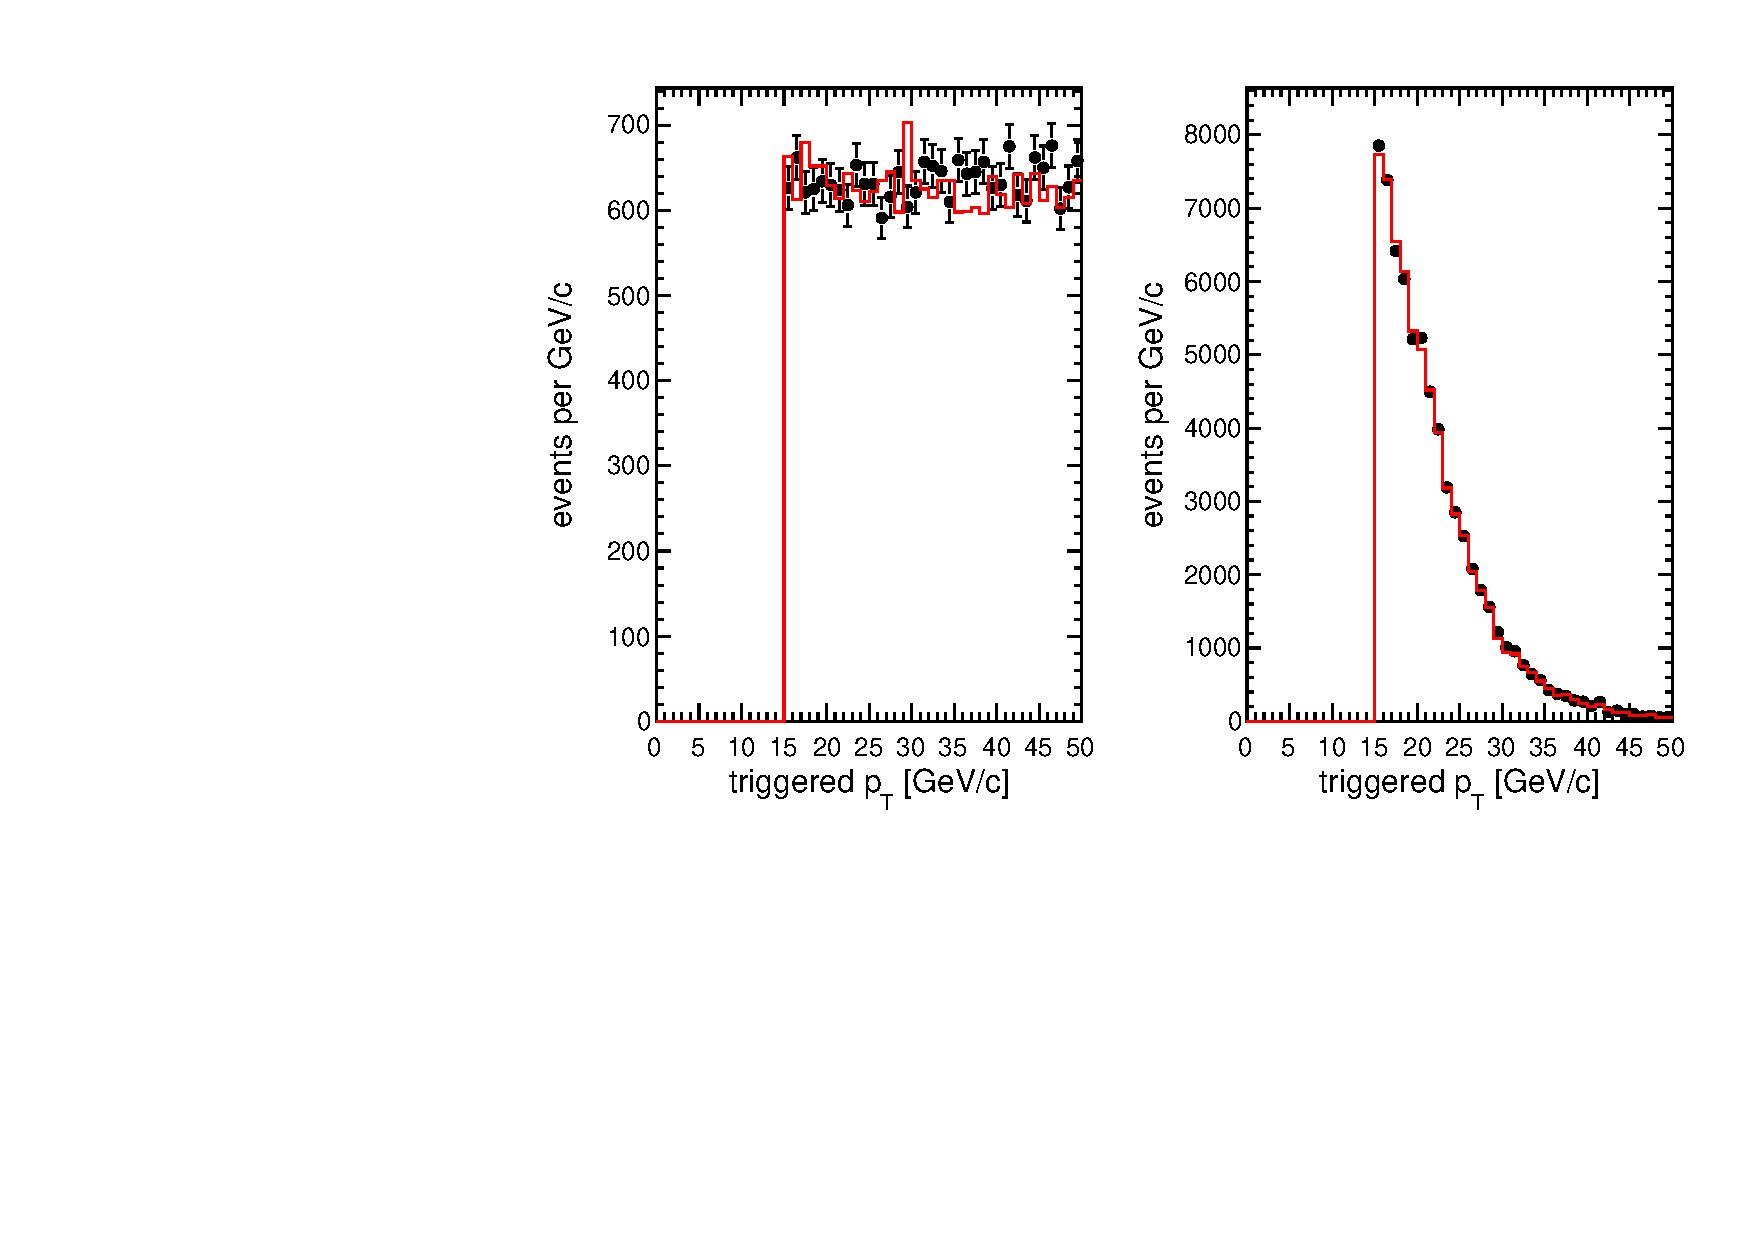
\includegraphics[width=0.47\linewidth]{PLOTS/simulation_triggeredpt.pdf} \hfill
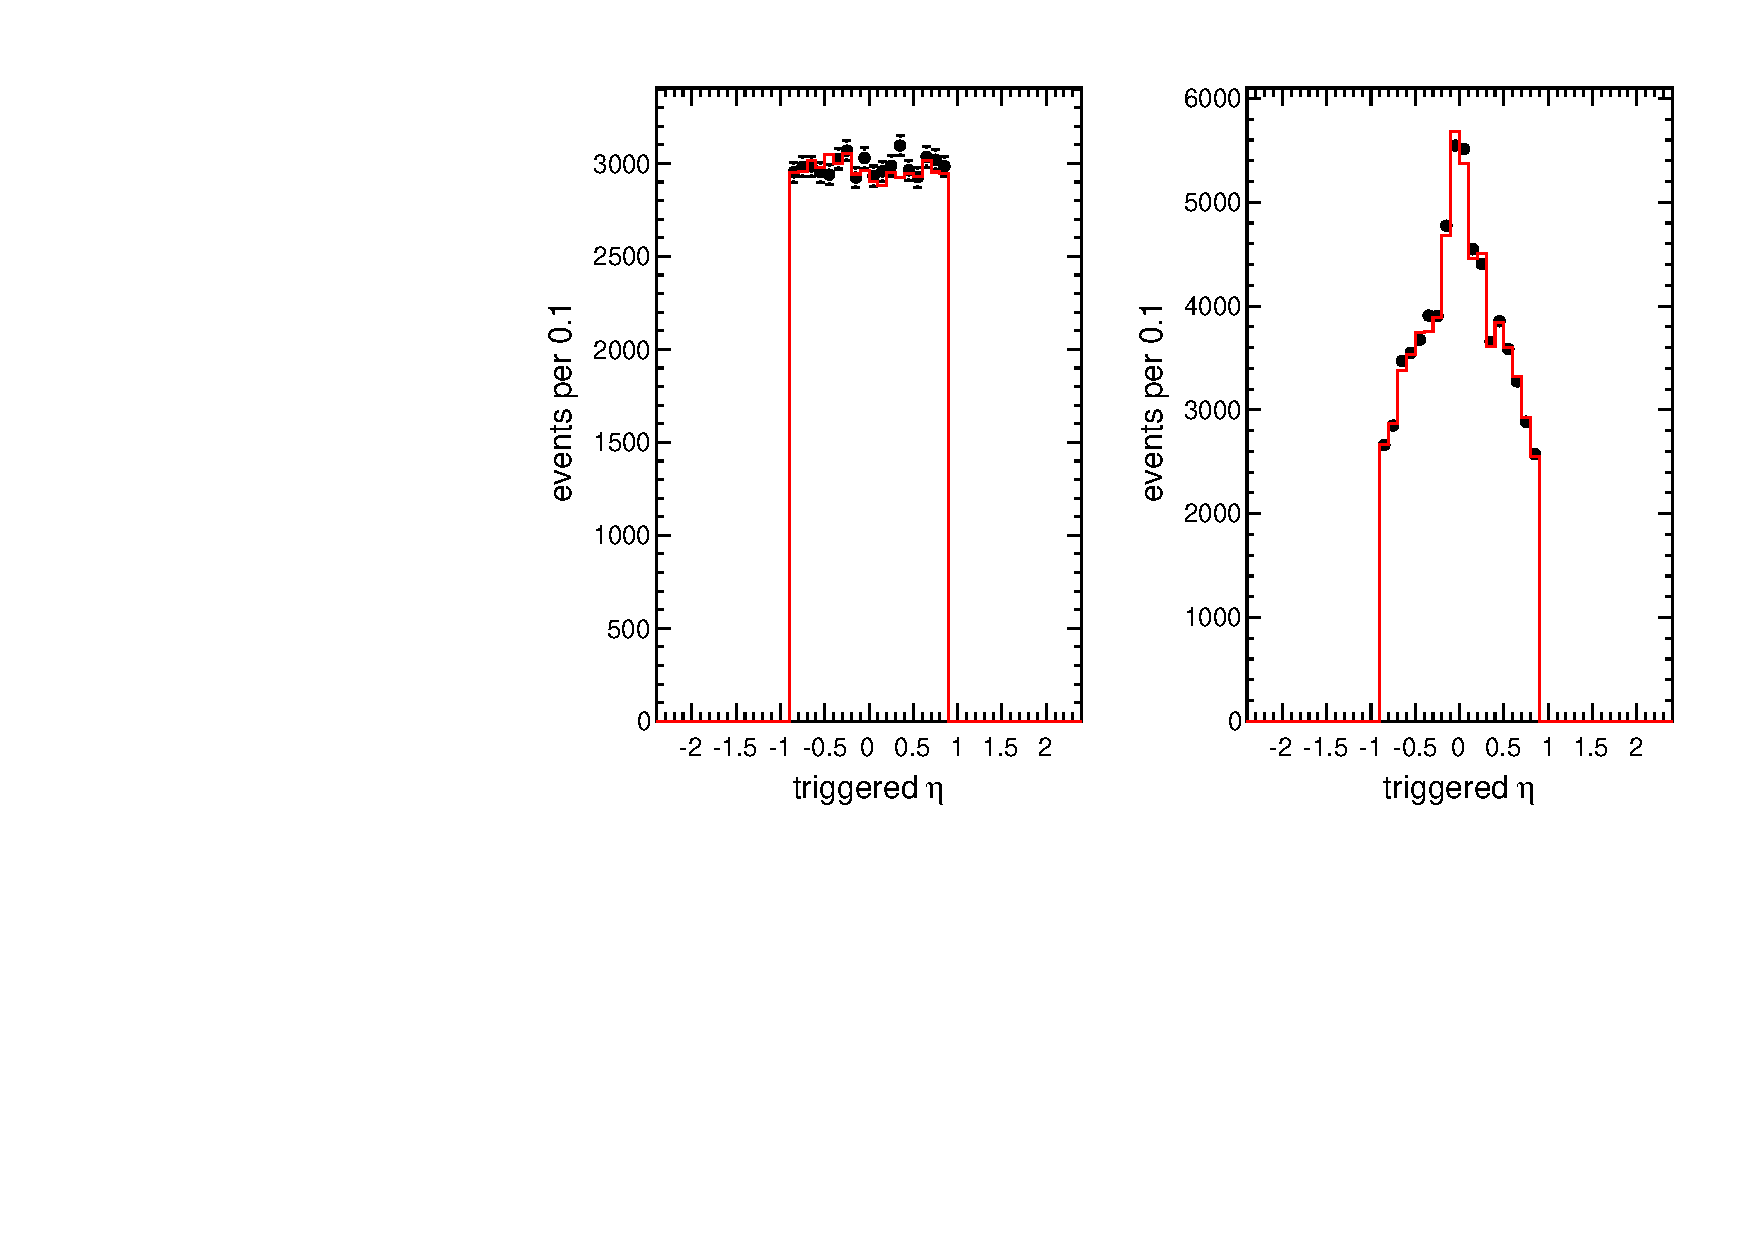
\includegraphics[width=0.47\linewidth]{PLOTS/simulation_triggeredeta.pdf}
\vspace{0.75 cm}
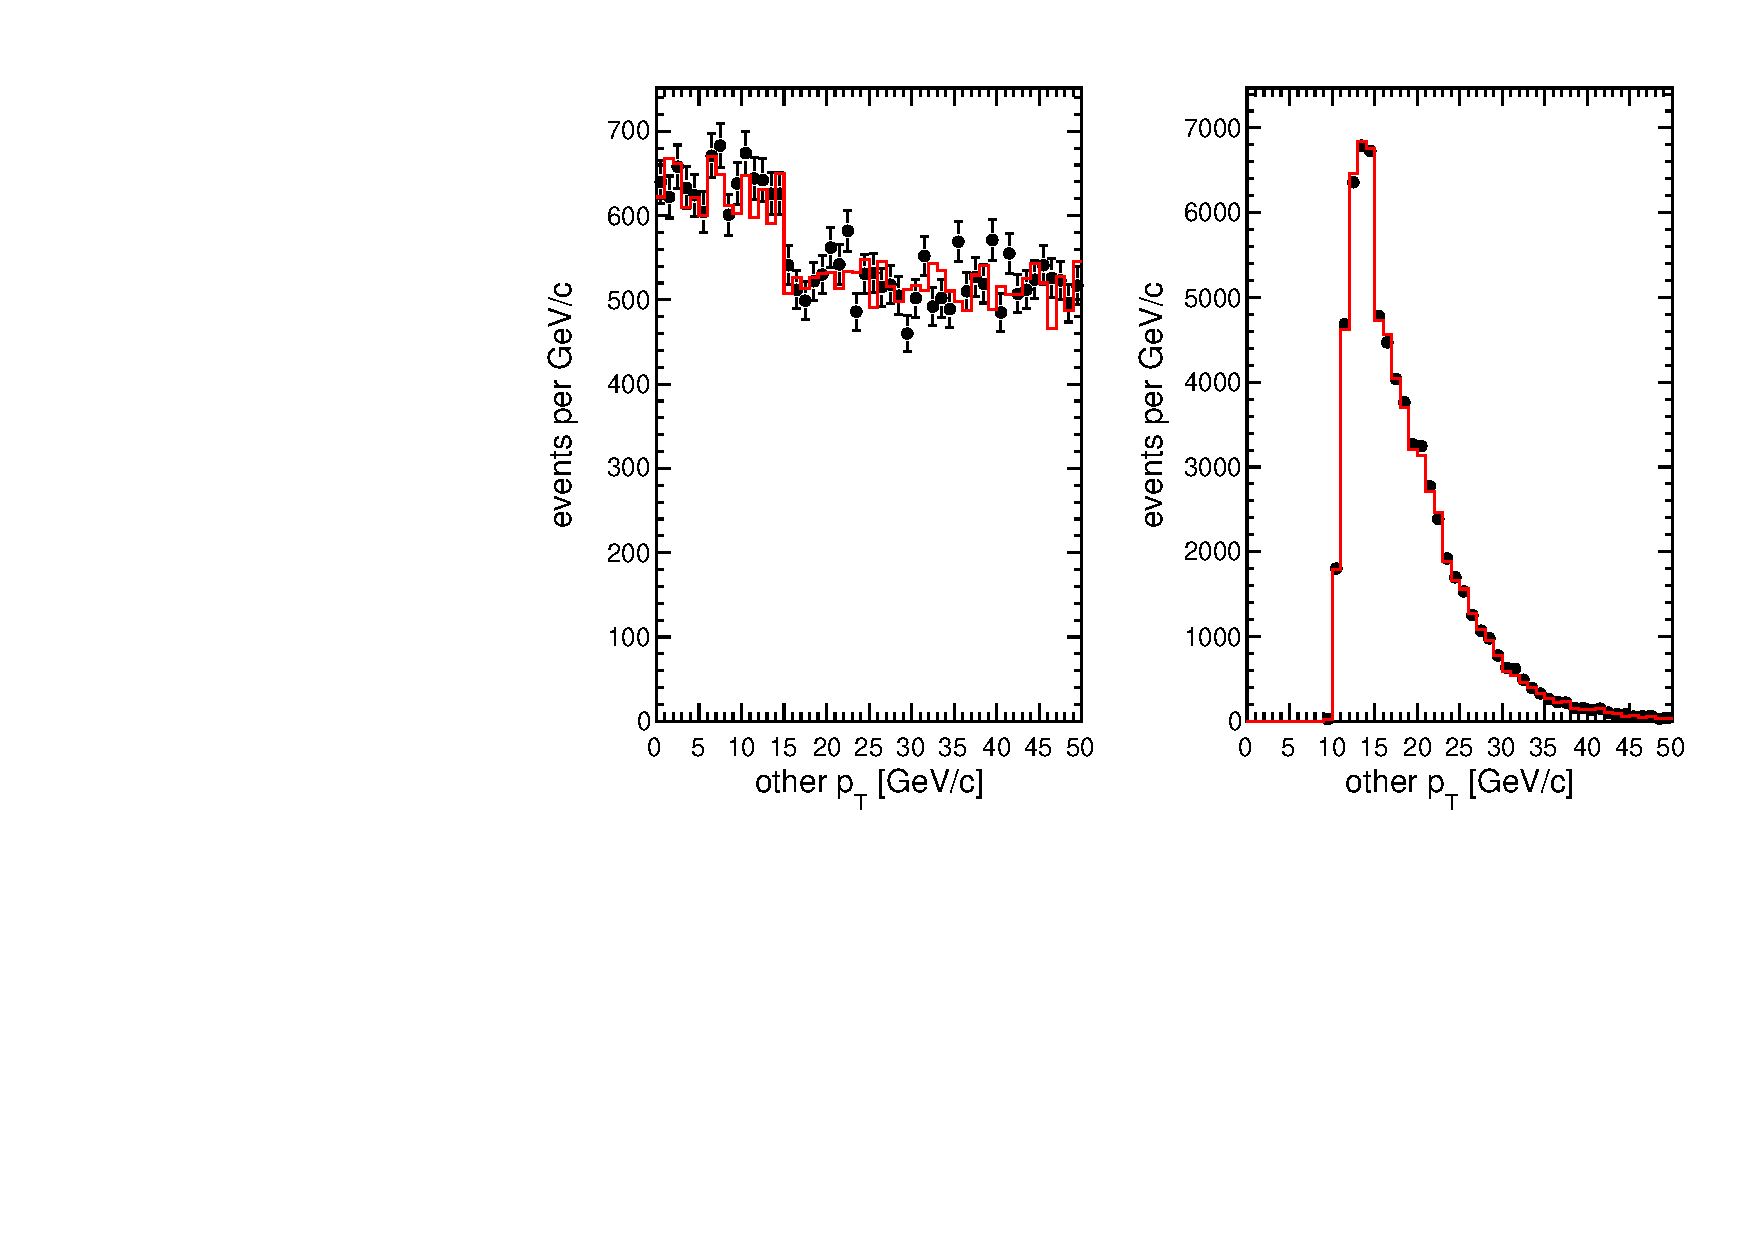
\includegraphics[width=0.47\linewidth]{PLOTS/simulation_otherpt.pdf} \hfill
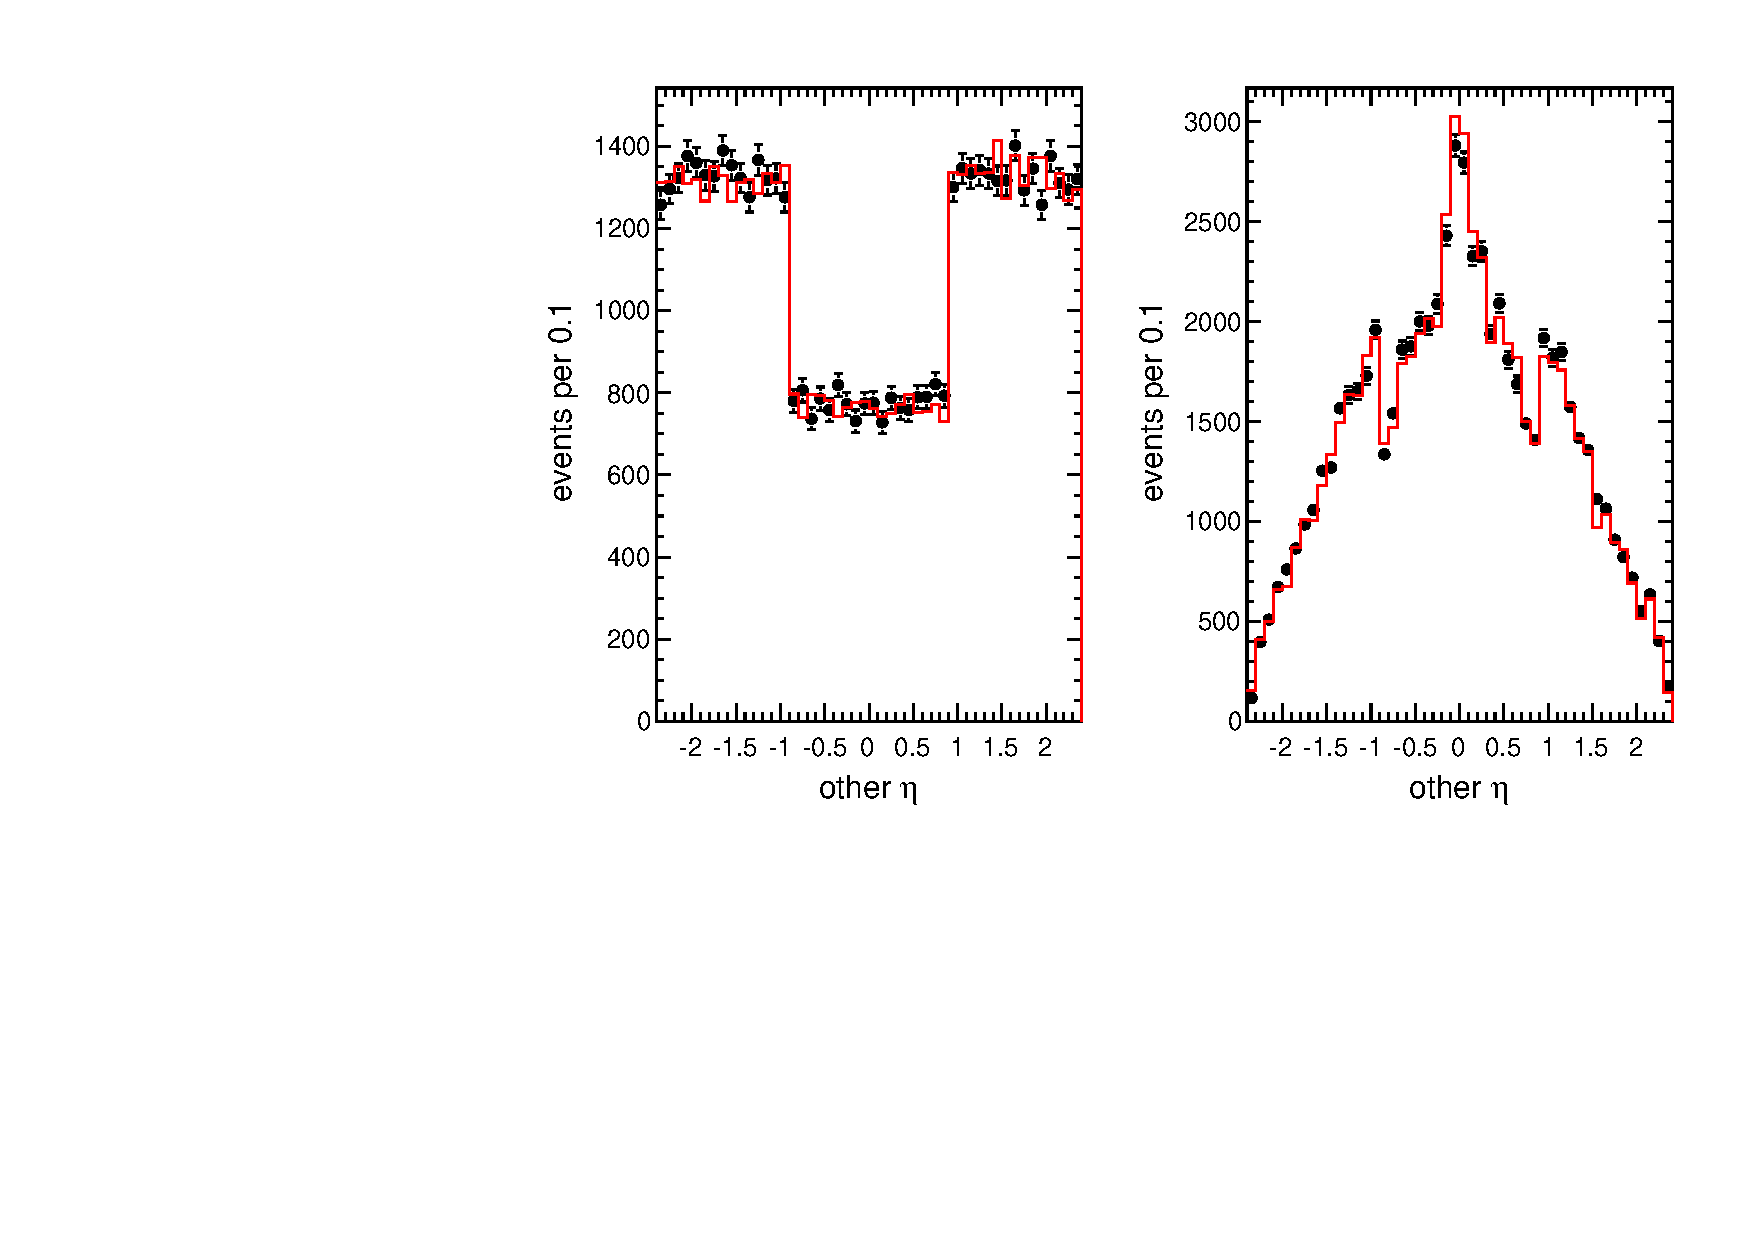
\includegraphics[width=0.47\linewidth]{PLOTS/simulation_othereta.pdf}
\caption{Toy Monte Carlo simulation of backgrounds in the dimuon-dimuon sample
  (black points), extrapolated from single-dimuons and
  dimuon-plus-muon background-enriched samples (red lines).  In each pair of plots, the
  left is a simplified model with uniform $p_T$ and $\eta$
  distributions and the right is a model with realistic $p_T$ and
  $\eta$ distributions.  The ``other dimuon'' distribution is
  depleted in the signal region, but the background-enriched sample
  is weighted to have the same distribution. \label{fig:simulation_pteta}}
\end{figure}

\subsection{Correlations in Fragmentation of the $b$-jets in $b\bar{b}$ Events}
\label{sec:appendix_factorizable_b_1}



Two-dimensional background mass templates for signal region (b-1) are constructed from 1D
background-enriched samples by forming a Cartesian product of the 1D dimuon mass 
distributions. Such a procedure is based on the assumption that the two dimuon mass 
distributions are independent in the signal region. For $b\bar{b}$ events (the dominant 
background in the (b-1) region), this is equivalent to assuming that the decays of the two
$b$-quarks and subsequent sculpting of their distributions with muon $p_T$ and $\eta$ 
cuts are independent. This seems fairly obvious as fragmentation of each $b$-quark should 
wash away any long range correlations before jet hadronization, yet we decided to verify
this explicitly.

\begin{figure}[tbh]
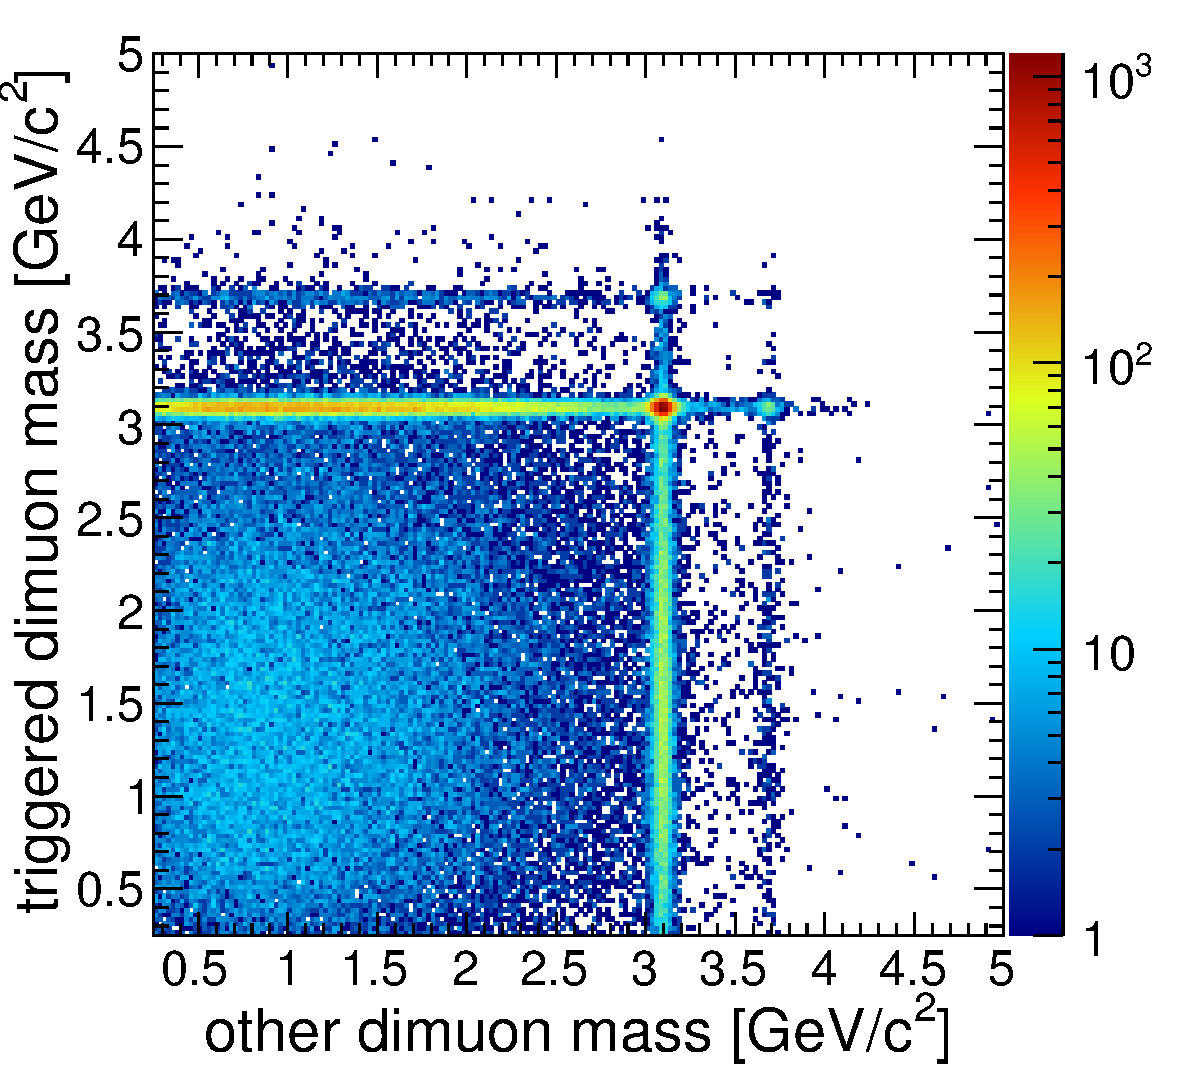
\includegraphics[height=6.2 cm]{PLOTS/mc_dimudimu_wholecontrol.pdf} \hfill
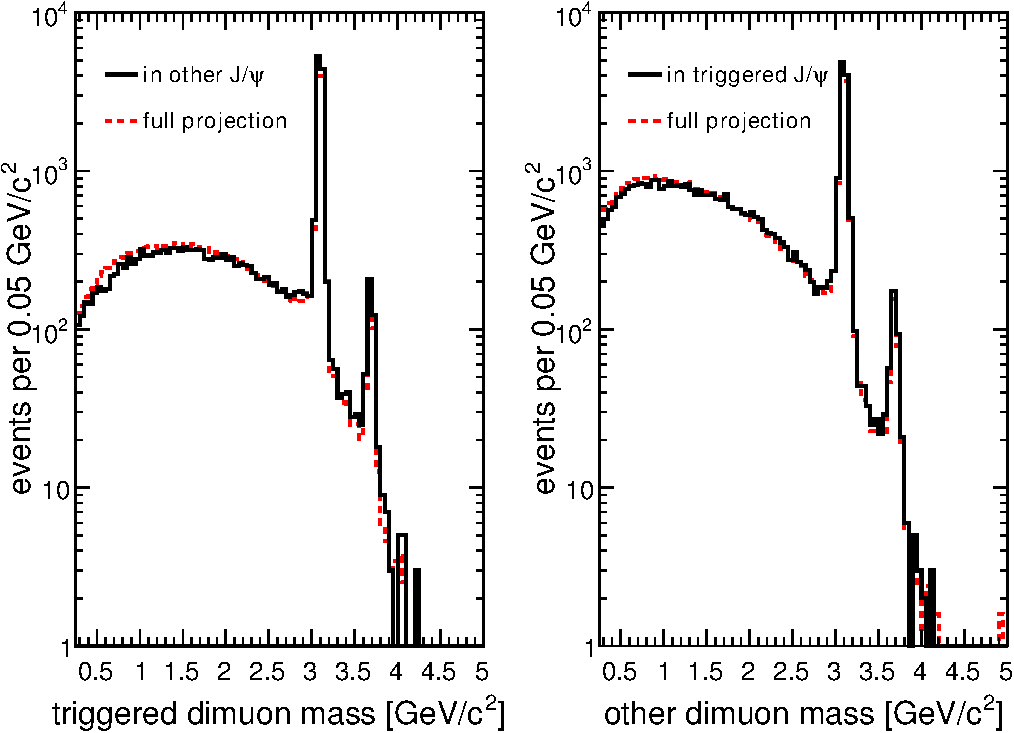
\includegraphics[height=6 cm]{PLOTS/mc_wholecontrolregions_factorize.pdf}
\caption{A Monte Carlo simulation of $b\bar{b} \to 2\mu \, 2\mu \, X$
  events to demonstrate the factorization of background mass
  distributions.  Left: the 2-D distribution.  Right: projected
  distributions in a slice around the $J/\psi$ and the whole
  distribution, normalized to equal areas. \label{fig:mc_dimudimu_wholecontrol}}
\end{figure}

To test this, we generated a large sample of $b\bar{b} \to 2\mu \,2\mu$ MC events 
(with full detector simulation), large enough to see any failure in factorization by eye. 
After reconstructing the dimuon candidates, in Fig.~\ref{fig:mc_dimudimu_wholecontrol}(a)
we plot the 2D distribution of invariant masses for the triggered and other dimuons. The
plot shows the expected asymmetry in the mass spectrum due to scalpting of the trigger
dimuon distribution by the requirement of an energetic muon, but no visible correlations
between the reconstructed masses of the two dimuons. To highlight any possible correlation 
between the invariant masses of the two dimuons, Fig.~\ref{fig:mc_dimudimu_wholecontrol}(b)
shows a 1D projection of the distribution onto the $y$-axis (invarant mass of the triggered 
dimuon) for the entire dataset (dashed red histogram) compared to the same projection but only
for events in a narrow slice in the $x$-direction near the $J/\psi$ mass (solid black line)
scaled up to have about the same normalization as the full projection. Again, the mass 
spectra are nearly identical showing no evidence of unexpected correlations. 
Fig.~\ref{fig:mc_dimudimu_wholecontrol}(c) shows the samilarly defined distributions, but 
projected onto the other dimuon mass axis.

\section{Categorization efficiencies in various benchmark models}
\label{sec:appendix_reco_eff}

The following tables present model acceptances as a function of
$\tilde{q}$ mass and $\gamma_D$ branching fraction to muons.
Table~\ref{tab:all_nmssm} presents an NMSSM sample point
(Sec.~\ref{sec:nmssm}), Table~\ref{tab:all_u1} presents SUSY dark
matter with a $\mathcal{U}(1)_{\mbox{\scriptsize dark}}$ symmetry
(Sec.~\ref{sec:susy_with_extra_u1}), and Tables~\ref{tab:all_squark2}
and \ref{tab:all_squark4} present the Dark Fermion Cascades model of
Sec.~\ref{sec:susy_with_dark_fermion_cascades}.  As a reminder, the
(a-1) signal region is exactly one mu-jet with exactly two muons and
$p_T^{\mu\mu} > 80$~GeV/$c$, (a-2) is exactly one mu-jet with exactly
four muons (two opposite-sign dimuons), (b-1) is exactly two mu-jets
each containing two muons (four total), and the $> 4\mu$ category
represents all events with more than four muons contained in mu-jets
(sum of (a-3), (b-2), and (c-1)).

\begin{table}[p]
\caption{NMSSM model acceptances in percent with $\mathcal{B}(a \to \mu\mu) = 100$\% hypothesis and separately for $m_{h}$ = 100 GeV/c$^2$ and $m_{a}$ = 2 GeV/c$^2$, where one of them is fixed and another one is variable (the case when $m_{h}$ = 100 GeV/c$^2$ and $m_{a}$ = 2 GeV/c$^2$ simultaneously duplicates the information in Table~\ref{tab:acceptance_benchmarks}).  Variable masses $m_{a}$ and $m_{h}$ are given in the first column (in GeV/$c^2$). Acceptance in regions with four muons ((a-2) and (b-1), labeled with asterisks) is restricted to the diagonal of the dimuon-dimuon space (within $5\sigma$ in detector resolution: $\sigma(m) = (0.026 + 0.0065\, b m)$~GeV/$c^2$, where $b=1$ for barrel and $b=2$ for endcap). \label{tab:all_nmssm}}

\begin{center}
\begin{tabular}{|c|c|c|c|c|}
\hline
\multirow{2}{*}{$m_{a}$} & \multicolumn{4}{|c|}{NMSSM with $m_{h}$ = 100 GeV/c$^2$}\\
\cline{2-5}
& (a-1) & (a-2) & (b-1) & $> 4 \mu$ \\
\hline
 0.3 &  0.9 &  0.0 & 40.6 &  0.0  \\
\hline
 0.5 &  1.4 &  0.0 & 30.9 &  0.0  \\
\hline
 1.0 &  1.5 &  0.0 & 25.9 &  0.0  \\
\hline
 2.0 &  1.7 &  0.0 & 23.8 &  0.0  \\
\hline
 4.0 &  1.6 &  0.0 & 23.6 &  0.0  \\
\hline
\end{tabular}
\end{center}

\begin{center}
\begin{tabular}{|c|c|c|c|c|}
\hline
\multirow{2}{*}{$m_{h}$} & \multicolumn{4}{|c|}{NMSSM with $m_{a}$ = 2 GeV/c$^2$}\\
\cline{2-5}
& (a-1) & (a-2) & (b-1) & $> 4 \mu$ \\
\hline
  85 &  1.2 &  0.0 & 20.4 &  0.0  \\
\hline
 100 &  1.7 &  0.0 & 23.8 &  0.0  \\
\hline
 120 &  2.5 &  0.0 & 28.9 &  0.0  \\
\hline
\end{tabular}
\end{center}
\end{table}

\begin{table}[p]
\caption{Dark matter with $\mathcal{U}(1)_{\mbox{\scriptsize dark}}$ model acceptances (\%) for four sample
$\mathcal{B}(a \to \mu\mu)$ hypotheses and two masses of $\gamma_{dark}$ (the case when $\mathcal{B}(a \to \mu\mu) = 100$\%, $m_{\tilde{g}} = 1200$ GeV/$c^2$, and $m_{\gamma_{dark}}$ = 1.0 GeV/c$^2$ duplicates information in
Table~\ref{tab:acceptance_benchmarks}).  The gluino, which is the top of the cascade produced in the $pp$ collision,
has a mass given in the first column (in GeV/$c^2$), $m(\tilde{\chi}_{\mbox{\scriptsize dark}}) =300$ GeV/c$^2$. Acceptance in regions with four muons ((a-2) and (b-1), labeled
with asterisks) is restricted to the diagonal of the dimuon-dimuon space (within $5\sigma$ in detector
resolution: $\sigma(m) = (0.026 + 0.0065\, b m)$~GeV/$c^2$, where $b=1$ for barrel
and $b=2$ for endcap). \label{tab:all_u1}}

\begin{center}
\begin{tabular}{|c|c|c|c|c|c|c|c|c|}
\hline
\multirow{3}{*}{$\tilde{g}$ mass} & \multicolumn{8}{|c|}{U(1) with $m_{\gamma_{dark}}$ = 1.0 GeV/c$^2$}\\
\cline{2-9}
& \multicolumn{4}{|c|}{Br($a \to \mu\mu$) = 100\%} & \multicolumn{4}{|c|}{Br($a \to \mu\mu$) = 50\%} \\
\cline{2-9}
& (a-1) & (a-2) & (b-1) & $> 4 \mu$ & (a-1) & (a-2) & (b-1) & $> 4 \mu$ \\
\hline
 500 &  5.9 &  4.2 & 14.3 & 40.0 & 10.4 &  3.4 &  9.0 &  6.3 \\
\hline
 600 &  6.0 &  4.5 & 14.1 & 41.7 & 11.3 &  3.3 &  9.1 &  6.2 \\
\hline
 800 &  6.6 &  4.8 & 15.2 & 43.2 & 12.7 &  3.3 &  9.7 &  6.4 \\
\hline
1000 &  7.4 &  4.9 & 15.3 & 44.1 & 13.9 &  3.9 & 10.5 &  6.8 \\
\hline
1200 &  7.4 &  5.1 & 15.4 & 45.3 & 14.6 &  4.1 & 10.0 &  7.6 \\
\hline
\end{tabular}
\begin{tabular}{|c|c|c|c|c|c|c|c|c|}
\hline
\multirow{2}{*}{$\tilde{g}$ mass} & \multicolumn{4}{|c|}{Br($a \to \mu\mu$) = 33\%} & \multicolumn{4}{|c|}{Br($a \to \mu\mu$) = 20\%} \\
\cline{2-9}
& (a-1) & (a-2) & (b-1) & $> 4 \mu$ & (a-1) & (a-2) & (b-1) & $> 4 \mu$ \\
\hline
 500 &  8.8 &  1.8 &  4.8 &  1.9 &  6.4 &  0.9 &  2.1 &  0.5 \\
\hline
 600 &  9.3 &  2.0 &  5.4 &  2.0 &  7.0 &  1.0 &  2.3 &  0.5 \\
\hline
 800 & 11.1 &  2.0 &  5.4 &  2.2 &  8.2 &  0.8 &  2.7 &  0.4 \\
\hline
1000 & 12.7 &  2.3 &  5.7 &  2.2 &  9.1 &  0.9 &  2.4 &  0.6 \\
\hline
1200 & 13.0 &  2.5 &  5.6 &  2.3 & 10.2 &  1.2 &  2.6 &  0.5 \\
\hline
\end{tabular}
\end{center}

\begin{center}
\begin{tabular}{|c|c|c|c|c|c|c|c|c|}
\hline
\multirow{2}{*}{$\tilde{g}$ mass} & \multicolumn{8}{|c|}{U(1) with $m_{\gamma_{dark}}$ = 0.5 GeV/c$^2$}\\
\cline{2-9}
& \multicolumn{4}{|c|}{Br($a \to \mu\mu$) = 100\%} & \multicolumn{4}{|c|}{Br($a \to \mu\mu$) = 50\%}\\
\cline{2-9}
& (a-1) & (a-2) & (b-1) & $> 4 \mu$ & (a-1) & (a-2) & (b-1) & $> 4 \mu$ \\
\hline
 500 &  4.9 &  3.8 & 19.0 & 39.9 & 10.9 &  3.1 & 10.2 &  6.3 \\
\hline
 600 &  5.3 &  3.7 & 19.1 & 41.2 & 11.6 &  3.2 & 10.7 &  6.2 \\
\hline
 800 &  5.5 &  4.3 & 19.7 & 42.6 & 12.7 &  3.6 & 11.5 &  6.6 \\
\hline
1000 &  6.3 &  4.3 & 19.7 & 43.3 & 14.2 &  3.6 & 11.8 &  6.4 \\
\hline
1200 &  6.6 &  4.3 & 18.4 & 44.6 & 14.8 &  4.0 & 11.7 &  7.3 \\
\hline
\end{tabular}
\begin{tabular}{|c|c|c|c|c|c|c|c|c|c|c|c|c|}
\hline
\multirow{2}{*}{$\tilde{g}$ mass} & \multicolumn{4}{|c|}{Br($a \to \mu\mu$) = 33\%} & \multicolumn{4}{|c|}{Br($a \to \mu\mu$) = 20\%}\\
\cline{2-9}
& (a-1) & (a-2) & (b-1) & $> 4 \mu$ & (a-1) & (a-2) & (b-1) & $> 4 \mu$ \\
\hline
 500 &  9.6 &  1.6 &  5.8 &  1.8 &  7.5 &  0.6 &  2.7 &  0.5 \\
\hline
 600 & 10.0 &  2.3 &  6.0 &  2.0 &  7.6 &  0.8 &  2.9 &  0.5 \\
\hline
 800 & 11.1 &  2.1 &  6.3 &  2.1 &  8.7 &  0.9 &  2.8 &  0.5 \\
\hline
1000 & 13.0 &  2.5 &  6.6 &  2.0 &  9.9 &  0.9 &  3.2 &  0.6 \\
\hline
1200 & 13.6 &  2.2 &  6.5 &  2.2 & 10.6 &  0.9 &  3.0 &  0.7 \\
\hline
\end{tabular}
\end{center}

\end{table}

\begin{table}[p]
\caption{Dark Fermion Cascades model acceptances (\%) with only $\gamma_{D} \to \mu\mu$ (no $h_{D} \to \gamma_{D}\gamma_{D} \to 4\mu$), 
for four sample $\mathcal{B}(a \to \mu\mu)$ hypotheses (the case when $\mathcal{B}(a \to \mu\mu) = 100$\% and $m_{\tilde{q}} = 400$ GeV/$c^2$ 
duplicates information in Table~\ref{tab:acceptance_benchmarks}). The squark, which is the top of the cascade produced in the $pp$ collision, 
has a mass given in the first column (in GeV/$c^2$).  
Acceptance in regions with four muons ((a-2) and (b-1), labeled with asterisks) is restricted to the diagonal of the 
dimuon-dimuon space (within $5\sigma$ in detector resolution: $\sigma(m) = (0.026 + 0.0065\, b m)$~GeV/$c^2$, 
where $b=1$ for barrel and $b=2$ for endcap). \label{tab:all_squark2}}

\begin{center}
\begin{tabular}{|c|c|c|c|c|c|c|c|c|}
\hline
\multirow{3}{*}{$\tilde{q}$ mass} & \multicolumn{8}{|c|}{$n_2 (\to n_1 \gamma_{D})$}\\
\cline{2-9}
& \multicolumn{4}{|c|}{Br($\gamma_{D} \to \mu\mu$) = 100\%} & \multicolumn{4}{|c|}{Br($\gamma_{D} \to \mu\mu$) = 50\%}\\
\cline{2-9}
& (a-1) & (a-2) & (b-1) & $> 4 \mu$ & (a-1) & (a-2) & (b-1) & $> 4 \mu$ \\
\hline
200 &  8.1 &  0.9 & 25.0 &  0.2 &  6.7 &  0.2 &  6.6 &  0.0 \\
\hline
250 & 11.5 &  0.9 & 31.1 &  0.2 & 10.1 &  0.1 &  7.9 &  0.0 \\
\hline
300 & 13.6 &  1.0 & 35.1 &  0.2 & 13.1 &  0.2 &  9.3 &  0.0 \\
\hline
350 & 15.8 &  0.9 & 38.2 &  0.4 & 16.0 &  0.2 & 10.0 &  0.0 \\
\hline
400 & 17.4 &  0.9 & 40.6 &  0.3 & 18.0 &  0.2 & 10.4 &  0.0 \\
\hline
450 & 18.4 &  0.8 & 42.0 &  0.3 & 20.6 &  0.2 & 10.8 &  0.0 \\
\hline
500 & 19.8 &  0.9 & 43.5 &  0.3 & 21.9 &  0.3 & 11.7 &  0.0 \\
\hline
550 & 20.4 &  0.6 & 43.0 &  0.4 & 22.7 &  0.2 & 11.3 &  0.0 \\
\hline
600 & 21.5 &  0.7 & 43.3 &  0.3 & 24.6 &  0.1 & 11.1 &  0.0 \\
\hline
650 & 21.6 &  0.7 & 43.3 &  0.4 & 24.7 &  0.2 & 11.4 &  0.0 \\
\hline
\end{tabular}
\begin{tabular}{|c|c|c|c|c|c|c|c|c|}
\hline
\multirow{2}{*}{$\tilde{q}$ mass} & \multicolumn{4}{|c|}{Br($\gamma_{D} \to \mu\mu$) = 33\%} & \multicolumn{4}{|c|}{Br($\gamma_{D} \to \mu\mu$) = 20\%}\\
\cline{2-9}
& (a-1) & (a-2) & (b-1) & $> 4 \mu$ & (a-1) & (a-2) & (b-1) & $> 4 \mu$ \\
\hline
200 &  5.2 &  0.1 &  2.7 &  0.0 &  3.2 &  0.1 &  1.1 &  0.0 \\
\hline
250 &  7.1 &  0.1 &  3.8 &  0.0 &  5.5 &  0.0 &  1.6 &  0.0 \\
\hline
300 & 10.6 &  0.1 &  4.0 &  0.0 &  7.2 &  0.0 &  1.5 &  0.0 \\
\hline
350 & 12.2 &  0.1 &  4.3 &  0.0 &  8.7 &  0.0 &  1.6 &  0.0 \\
\hline
400 & 14.2 &  0.0 &  4.7 &  0.0 &  9.8 &  0.0 &  1.8 &  0.0 \\
\hline
450 & 16.1 &  0.1 &  4.6 &  0.0 & 10.8 &  0.0 &  1.6 &  0.0 \\
\hline
500 & 17.1 &  0.1 &  5.2 &  0.0 & 12.1 &  0.0 &  1.9 &  0.0 \\
\hline
550 & 18.5 &  0.0 &  5.1 &  0.0 & 12.3 &  0.0 &  1.9 &  0.0\\
\hline
600 & 19.5 &  0.1 &  5.0 &  0.0 & 12.9 &  0.0 &  1.8 &  0.0\\
\hline
650 & 20.1 &  0.1 &  5.3 &  0.0 & 14.0 &  0.0 &  2.0 &  0.0\\
\hline
\end{tabular}
\end{center}

\end{table}

\begin{table}[p]
\caption{Dark Fermion Cascades model acceptances (\%) with only $h_{D} \to \gamma_{D}\gamma_{D} \to 4\mu$ (no direct 
$\gamma_{D} \to \mu\mu$), for four sample $\mathcal{B}(a \to \mu\mu)$ hypotheses (the case when $\mathcal{B}(a \to \mu\mu) = 100$\% 
and $m_{\tilde{q}} = 400$ GeV/$c^2$ duplicates information in Table~\ref{tab:acceptance_benchmarks}).  The squark, which is the top 
of the cascade produced in the $pp$ collision, has a mass given in the first column (in GeV/$c^2$).  
Acceptance in regions with four muons ((a-2) and (b-1), labeled with asterisks) is restricted to the diagonal of 
the dimuon-dimuon space (within $5\sigma$ in detector resolution: 
$\sigma(m) = (0.026 + 0.0065\, b m)$~GeV/$c^2$, where $b=1$ for barrel and $b=2$ for 
endcap). \label{tab:all_squark4}}

\begin{center}
\begin{tabular}{|c|c|c|c|c|c|c|c|c|}
\hline
\multirow{3}{*}{$\tilde{q}$ mass} & \multicolumn{8}{|c|}{$n_2 \to n_1 h_{D}(\to 2 \gamma_{D})$}\\
\cline{2-9}
& \multicolumn{4}{|c|}{Br($\gamma_{D} \to \mu\mu$) = 100\%} & \multicolumn{4}{|c|}{Br($\gamma_{D} \to \mu\mu$) = 50\%}\\
\cline{2-9}
& (a-1) & (a-2) & (b-1) & $> 4 \mu$ & (a-1) & (a-2) & (b-1) & $> 4 \mu$ \\
\hline
200 &  0.3 &  5.9 &  0.7 & 43.1 &  1.3 &  4.3 &  4.0 &  8.4 \\
\hline
250 &  0.4 &  6.1 &  0.6 & 52.1 &  2.6 &  4.6 &  5.3 & 10.6 \\
\hline
300 &  0.6 &  6.8 &  0.6 & 56.8 &  4.0 &  6.1 &  6.1 & 11.6 \\
\hline
350 &  0.7 &  6.9 &  0.6 & 60.2 &  5.0 &  6.1 &  7.0 & 12.5 \\
\hline
400 &  0.9 &  6.6 &  0.7 & 63.1 &  7.0 &  6.3 &  7.1 & 13.5 \\
\hline
450 &  1.0 &  6.7 &  0.6 & 64.2 &  9.4 &  6.7 &  7.5 & 13.6 \\
\hline
500 &  1.1 &  7.3 &  0.5 & 64.5 &  9.7 &  6.6 &  7.3 & 13.9 \\
\hline
550 &  1.5 &  7.5 &  0.7 & 64.8 & 11.2 &  6.4 &  7.6 & 14.0 \\
\hline
600 &  1.8 &  7.6 &  0.7 & 64.1 & 11.5 &  6.6 &  7.8 & 13.6 \\
\hline
650 &  2.0 &  7.8 &  0.8 & 62.9 & 13.1 &  6.6 &  7.2 & 14.0 \\
\hline
\end{tabular}
\begin{tabular}{|c|c|c|c|c|c|c|c|c|}
\hline
\multirow{2}{*}{$\tilde{q}$ mass} & \multicolumn{4}{|c|}{Br($\gamma_{D} \to \mu\mu$) = 33\%} & \multicolumn{4}{|c|}{Br($\gamma_{D} \to \mu\mu$) = 20\%}\\
\cline{2-9}
& (a-1) & (a-2) & (b-1) & $> 4 \mu$ & (a-1) & (a-2) & (b-1) & $> 4 \mu$ \\
\hline
200 &  1.3 &  2.3 &  2.9 &  2.5 &  1.2 &  1.1 &  1.5 &  0.7 \\
\hline
250 &  2.5 &  2.9 &  3.8 &  3.6 &  2.0 &  1.2 &  2.0 &  1.0 \\
\hline
300 &  4.2 &  3.6 &  4.4 &  4.0 &  3.5 &  1.5 &  2.7 &  1.3 \\
\hline
350 &  5.7 &  3.7 &  4.6 &  4.2 &  4.7 &  1.8 &  2.9 &  1.3 \\
\hline
400 &  6.6 &  3.9 &  5.6 &  4.5 &  5.9 &  1.7 &  2.8 &  1.1 \\
\hline
450 &  8.9 &  3.9 &  5.3 &  4.5 &  8.0 &  1.7 &  2.8 &  1.1 \\
\hline
500 & 10.2 &  4.1 &  5.7 &  4.6 &  9.3 &  1.7 &  2.9 &  1.2 \\
\hline
550 & 12.1 &  4.0 &  5.4 &  4.0 &  10.4 & 1.6 &  2.8 &  1.2 \\
\hline
600 & 13.5 &  3.9 &  5.4 &  4.7 &  11.3 & 1.6 &  2.9 &  1.2 \\
\hline
650 & 13.4 &  3.6 &  5.2 &  4.5 &  11.6 & 1.7 &  2.8 &  1.2 \\
\hline
\end{tabular}
\end{center}

\end{table}

%% As a reminder, the signal regions are:
%% \begin{enumerate}\renewcommand{\labelenumi}{(\alph{enumi})}
%% \item only one mu-jet per event:
%% \begin{enumerate}\renewcommand{\labelenumii}{(a-\arabic{enumii})}
%% \item the mu-jet contains exactly two muons with $p_T^{\mu\mu} > 80$~GeV/$c$;
%% \item the mu-jet contains exactly four muons (two dimuons);
%% \item the mu-jet contains more than four muons;
%% \end{enumerate}

%% \item exactly two mu-jets per event:
%% \begin{enumerate}\renewcommand{\labelenumii}{(b-\arabic{enumii})}
%% \item both mu-jets contain exactly two muons;
%% \item either mu-jet or both mu-jets contain more than two muons;
%% \end{enumerate}

%% \item more than two mu-jets per event.
%% \end{enumerate}
%% For brevity, the high dimuon-multiplicity regions, (a-3), (b-2), and
%% (c), have been merged into a single ``$> 4\mu$'' column.  No cuts are
%% placed on the presence or absence of {\it ungrouped} muons.

\section{Event displays}
\label{sec:appendix_event_displays}

Figures~\ref{fig:quadmu_wholecontrol}
and \ref{fig:dimudimu_wholecontrol} show sample events in the (a-2)
and (b-1) control regions.  There were no events with equal-mass
dimuons (or any larger numbers of muons than four).

\begin{figure}[p]
\begin{center}
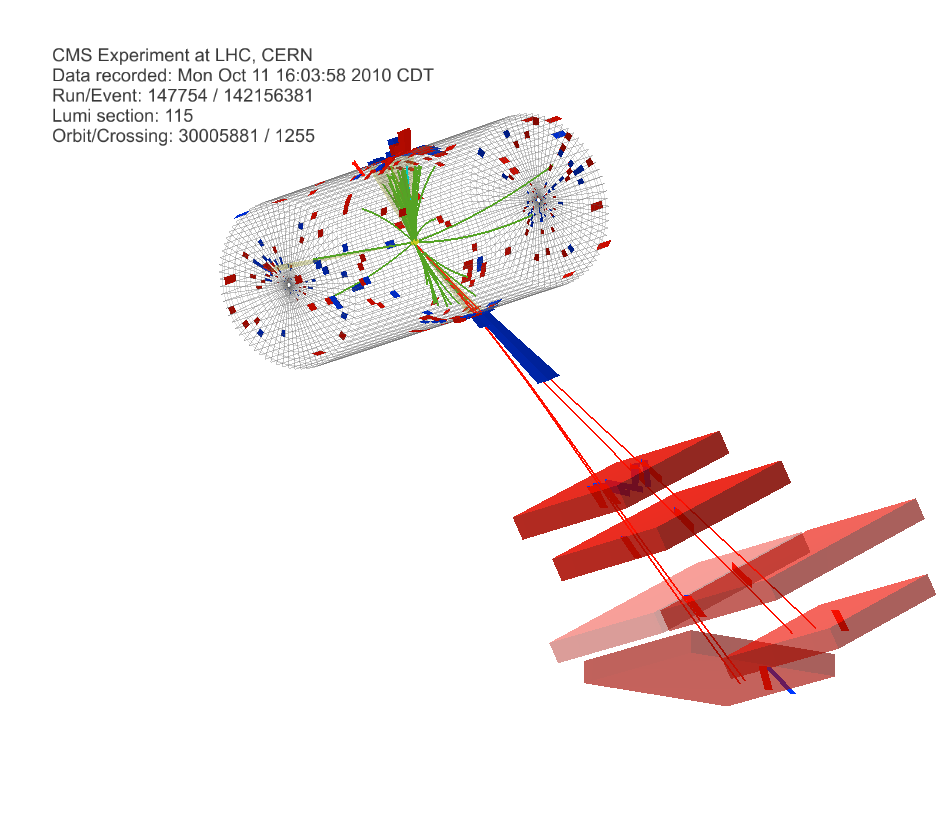
\includegraphics[width=0.65\linewidth]{PLOTS/quadmu_control_eventdisplay.png}
\end{center}
\caption{The event in the (a-2) region.  The two dimuons are
not close enough in mass to be decays of the same on-shell $m_1$ boson
(and therefore belong to the off-diagonal control).  \label{fig:quadmu_wholecontrol}}
\end{figure}

\begin{figure}[p]
\begin{center}
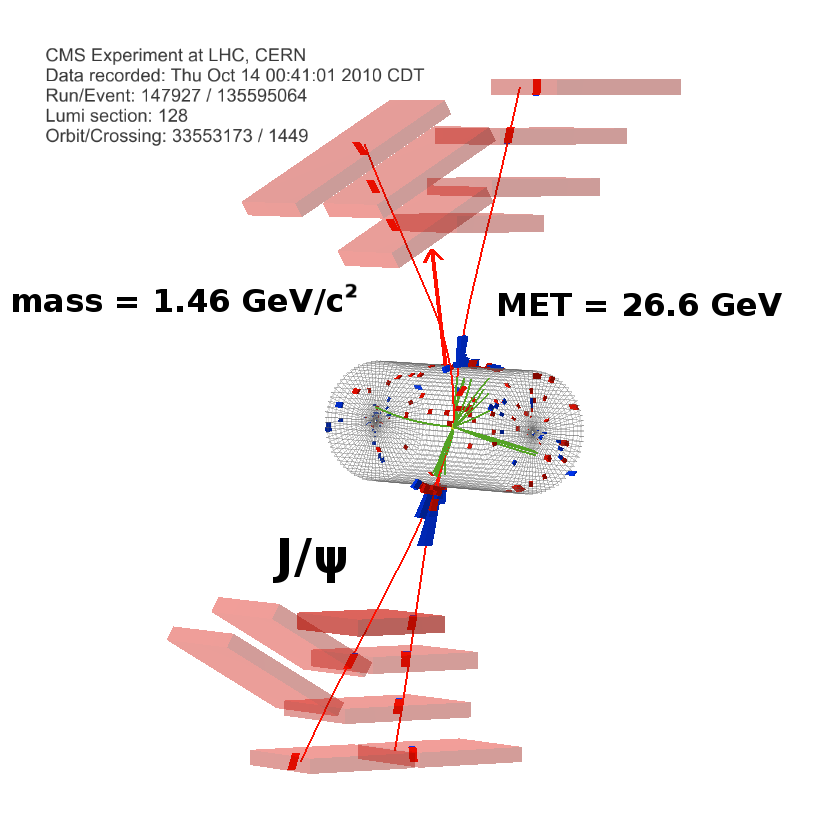
\includegraphics[width=0.65\linewidth]{PLOTS/dimudimu_control_eventdisplay.png}
\end{center}

\caption{An event in the (b-1) region.  The two dimuons are not close
enough in mass to be decays of the same on-shell $m_1$ boson (and
therefore belong to the off-diagonal control). \label{fig:dimudimu_wholecontrol}}
\end{figure}

\section{Tables of background templates parameters}
\label{sec:bg_fits_numbers}

% eval `./tdr runtime -sh`
% ./tdr --styl note b AN-10-462

\begin{table}[htb]
\caption{$R^1_2$ BG template fit results.}
\begin{center}
\begin{tabular}{|l|c|}
\hline
$\sigma_{J/\psi} $ & $  0.0279\pm 0.0013$\\
$\sigma_{\omega} $ & $  0.01$\\
$p_{1/m^{2}} $ & $  135\pm 65$\\
$p_{\omega} $ & $  16.3\pm 6.3$\\
$p_{\phi} $ & $  8.9\pm 5.8$\\
$p_{J/\psi} $ & $  492\pm 23$\\
$p_{\psi'} $ & $  21.5\pm 5.6$\\
$p_{poly} $ & $  1084\pm 75$\\
$\sigma_{\phi} $ & $  0.01$\\
$p_{1} $ & $  0.57\pm 0.39$\\
$p_{2} $ & $  1.00$\\
$p_{3} $ & $  0.86\pm 0.78$\\
$p_{4} $ & $  0.00$\\
$p_{5} $ & $  0.00$\\
$p_{6} $ & $  0.080\pm 0.028$\\
$\sigma_{\psi'} $ & $  0.03$\\
\hline
\end{tabular}
\end{center}
\end{table}

\begin{table}[htb]
\caption{$R^1_2$ BG template fit correlation matrix.}
{\tiny
\begin{center}
\begin{tabular}{|l|rrrrrrrrrr|}
\hline
 & $\sigma_{J/\psi}$ & $p_{1/m^{2}}$ & $p_{\omega}$ & $p_{\phi}$ & $p_{J/\psi}$ & $p_{\psi'}$ & $p_{poly}$ & $p_{1}$ & $p_{3}$ & $p_{6}$\\
\hline
$\sigma_{J/\psi}$ & $1.000$ & $0.055$ & $-0.002$ & $-0.009$ & $0.136$ & $0.028$ & $-0.092$ & $-0.087$ & $-0.136$ & $0.078$\\
$p_{1/m^{2}}$ & $0.055$ & $1.000$ & $0.116$ & $0.039$ & $0.039$ & $0.063$ & $-0.874$ & $-0.897$ & $-0.716$ & $0.648$\\
$p_{\omega}$ & $-0.002$ & $0.116$ & $1.000$ & $0.032$ & $-0.002$ & $-0.001$ & $-0.152$ & $-0.101$ & $-0.037$ & $0.049$\\
$p_{\phi}$ & $-0.009$ & $0.039$ & $0.032$ & $1.000$ & $-0.007$ & $-0.010$ & $-0.091$ & $0.003$ & $0.062$ & $-0.038$\\
$p_{J/\psi}$ & $0.136$ & $0.039$ & $-0.002$ & $-0.007$ & $1.000$ & $0.021$ & $-0.067$ & $-0.062$ & $-0.097$ & $0.054$\\
$p_{\psi'}$ & $0.028$ & $0.063$ & $-0.001$ & $-0.010$ & $0.021$ & $1.000$ & $-0.085$ & $-0.095$ & $-0.131$ & $0.103$\\
$p_{poly}$ & $-0.092$ & $-0.874$ & $-0.152$ & $-0.091$ & $-0.067$ & $-0.085$ & $1.000$ & $0.816$ & $0.663$ & $-0.591$\\
$p_{1}$ & $-0.087$ & $-0.897$ & $-0.101$ & $0.003$ & $-0.062$ & $-0.095$ & $0.816$ & $1.000$ & $0.914$ & $-0.772$\\
$p_{3}$ & $-0.136$ & $-0.716$ & $-0.037$ & $0.062$ & $-0.097$ & $-0.131$ & $0.663$ & $0.914$ & $1.000$ & $-0.754$\\
$p_{6}$ & $0.078$ & $0.648$ & $0.049$ & $-0.038$ & $0.054$ & $0.103$ & $-0.591$ & $-0.772$ & $-0.754$ & $1.000$\\
\hline
\end{tabular}
\end{center}
}
\end{table}

\begin{table}[htb]
\caption{$R^1_4$ BG template fit results (mu+mu BG template).}
\begin{center}
\begin{tabular}{|l|c|}
\hline
$\sigma_{J/\psi} $ & $  0.0200\pm 0.0039$\\
$\sigma_{\omega} $ & $  0.01$\\
$p_{1/m^{2}} $ & $  76\pm 48$\\
$p_{\omega} $ & $  10.6\pm 4.7$\\
$p_{\phi} $ & $  18.7\pm 5.6$\\
$p_{J/\psi} $ & $  23.5\pm 5.2$\\
$p_{\psi'} $ & $  3.4\pm 2.1$\\
$p_{poly} $ & $  267\pm 52$\\
$\sigma_{\phi} $ & $  0.01$\\
$p_{1} $ & $  0.05\pm 0.60$\\
$p_{2} $ & $  1.00$\\
$p_{3} $ & $  0.00$\\
$p_{4} $ & $  0.00$\\
$p_{5} $ & $  0.04\pm 0.18$\\
$p_{6} $ & $  0.00\pm 0.99$\\
$p_{7} $ & $  0.00$\\
$p_{8} $ & $  0.00$\\
$p_{9} $ & $  0.0027\pm 0.0052$\\
$\sigma_{\psi'} $ & $  0.03$\\
\hline
\end{tabular}
\end{center}
\end{table}

\begin{table}[htb]
\caption{$R^1_4$ BG template fit correlation matrix (mu+mu BG template).}
{\tiny
\begin{center}
\begin{tabular}{|l|rrrrrrrrrrr|}
\hline
 & $\sigma_{J/\psi}$ & $p_{1/m^{2}}$ & $p_{\omega}$ & $p_{\phi}$ & $p_{J/\psi}$ & $p_{\psi'}$ & $p_{poly}$ & $p_{1}$ & $p_{5}$ & $p_{6}$ & $p_{9}$\\
\hline
$\sigma_{J/\psi}$ & $1.000$ & $0.063$ & $-0.004$ & $-0.012$ & $0.131$ & $-0.021$ & $-0.071$ & $-0.074$ & $-0.131$ & $0.108$ & $-0.035$\\
$p_{1/m^{2}}$ & $0.063$ & $1.000$ & $0.073$ & $-0.029$ & $0.059$ & $-0.110$ & $-0.929$ & $-0.952$ & $-0.495$ & $0.379$ & $-0.374$\\
$p_{\omega}$ & $-0.004$ & $0.073$ & $1.000$ & $0.023$ & $-0.004$ & $0.010$ & $-0.118$ & $-0.069$ & $0.030$ & $-0.037$ & $-0.013$\\
$p_{\phi}$ & $-0.012$ & $-0.029$ & $0.023$ & $1.000$ & $-0.011$ & $0.024$ & $-0.018$ & $0.045$ & $0.093$ & $-0.087$ & $0.029$\\
$p_{J/\psi}$ & $0.131$ & $0.059$ & $-0.004$ & $-0.011$ & $1.000$ & $-0.021$ & $-0.066$ & $-0.069$ & $-0.124$ & $0.103$ & $-0.033$\\
$p_{\psi'}$ & $-0.021$ & $-0.110$ & $0.010$ & $0.024$ & $-0.021$ & $1.000$ & $0.095$ & $0.133$ & $0.285$ & $-0.307$ & $0.076$\\
$p_{poly}$ & $-0.071$ & $-0.929$ & $-0.118$ & $-0.018$ & $-0.066$ & $0.095$ & $1.000$ & $0.911$ & $0.460$ & $-0.347$ & $0.355$\\
$p_{1}$ & $-0.074$ & $-0.952$ & $-0.069$ & $0.045$ & $-0.069$ & $0.133$ & $0.911$ & $1.000$ & $0.581$ & $-0.466$ & $0.383$\\
$p_{5}$ & $-0.131$ & $-0.495$ & $0.030$ & $0.093$ & $-0.124$ & $0.285$ & $0.460$ & $0.581$ & $1.000$ & $-0.977$ & $0.312$\\
$p_{6}$ & $0.108$ & $0.379$ & $-0.037$ & $-0.087$ & $0.103$ & $-0.307$ & $-0.347$ & $-0.466$ & $-0.977$ & $1.000$ & $-0.282$\\
$p_{9}$ & $-0.035$ & $-0.374$ & $-0.013$ & $0.029$ & $-0.033$ & $0.076$ & $0.355$ & $0.383$ & $0.312$ & $-0.282$ & $1.000$\\
\hline
\end{tabular}
\end{center}
}
\end{table}

\begin{table}[htb]
\caption{$R^1_4$ BG template fit results (track+track BG template).}
\begin{center}
\begin{tabular}{|l|c|}
\hline
$\mu_{peak} $ & $  0.592\pm 0.058$\\
$\sigma_{peak} $ & $  0.30\pm 0.11$\\
$p_{gaus} $ & $  140\pm 34$\\
$p_{poly} $ & $  259\pm 35$\\
$p_{1} $ & $  1.00\pm 0.74$\\
$p_{2} $ & $  1.00$\\
$p_{3} $ & $  0.00$\\
$p_{4} $ & $  0.163\pm 0.092$\\
$p_{5} $ & $  0.00$\\
$p_{6} $ & $  0.022\pm 0.021$\\
\hline
\end{tabular}
\end{center}
\end{table}

\begin{table}[htb]
\caption{$R^1_4$ BG template fit correlation matrix (track+track BG template).}
{\tiny
\begin{center}
\begin{tabular}{|l|rrrrrrr|}
\hline
 & $\mu_{peak}$ & $\sigma_{peak}$ & $p_{gaus}$ & $p_{poly}$ & $p_{1}$ & $p_{4}$ & $p_{6}$\\
\hline
$\mu_{peak}$ & $1.000$ & $-0.475$ & $-0.201$ & $0.191$ & $-0.017$ & $-0.137$ & $0.003$\\
$\sigma_{peak}$ & $-0.475$ & $1.000$ & $0.750$ & $-0.713$ & $0.017$ & $0.503$ & $-0.015$\\
$p_{gaus}$ & $-0.201$ & $0.750$ & $1.000$ & $-0.833$ & $0.030$ & $0.602$ & $-0.011$\\
$p_{poly}$ & $0.191$ & $-0.713$ & $-0.833$ & $1.000$ & $-0.028$ & $-0.573$ & $0.010$\\
$p_{1}$ & $-0.017$ & $0.017$ & $0.030$ & $-0.028$ & $1.000$ & $-0.006$ & $0.003$\\
$p_{4}$ & $-0.137$ & $0.503$ & $0.602$ & $-0.573$ & $-0.006$ & $1.000$ & $0.229$\\
$p_{6}$ & $0.003$ & $-0.015$ & $-0.011$ & $0.010$ & $0.003$ & $0.229$ & $1.000$\\
\hline
\end{tabular}
\end{center}
}
\end{table}

\begin{table}[htb]
\caption{$R^1_4$ BG template fit results (mu+track BG template).}
\begin{center}
\begin{tabular}{|l|c|}
\hline
$p_{poly} $ & $  1654\pm 41$\\
$p_{1} $ & $  0.435\pm 0.055$\\
$p_{2} $ & $  1.00$\\
$p_{3} $ & $  0.00$\\
$p_{4} $ & $  0.00$\\
$p_{5} $ & $  0.00$\\
$p_{6} $ & $  0.029\pm 0.012$\\
$p_{7} $ & $  0.0282\pm 0.0093$\\
\hline
\end{tabular}
\end{center}
\end{table}

\begin{table}[htb]
\caption{$R^1_4$ BG template fit correlation matrix (mu+track BG template).}
{\tiny
\begin{center}
\begin{tabular}{|l|rrrr|}
\hline
 & $p_{poly}$ & $p_{1}$ & $p_{6}$ & $p_{7}$\\
\hline
$p_{poly}$ & $1.000$ & $0.000$ & $0.000$ & $0.000$\\
$p_{1}$ & $0.000$ & $1.000$ & $-0.197$ & $0.060$\\
$p_{6}$ & $0.000$ & $-0.197$ & $1.000$ & $0.661$\\
$p_{7}$ & $0.000$ & $0.060$ & $0.661$ & $1.000$\\
\hline
\end{tabular}
\end{center}
}
\end{table}

\begin{table}[htb]
\caption{$R^1_4$ invariant mass BG template fit results.}
\begin{center}
\begin{tabular}{|l|c|}
\hline
$\mu_{peak1} $ & $  2.30\pm 0.10$\\
$\mu_{peak2} $ & $  4.31\pm 0.11$\\
$\sigma_{peak1} $ & $  0.701\pm 0.058$\\
$\sigma_{peak2} $ & $  0.707\pm 0.098$\\
$p_{gaus1} $ & $  443\pm 49$\\
$p_{gaus2} $ & $  411\pm 63$\\
$p_{poly} $ & $  372\pm 44$\\
$p_{1} $ & $  0.00$\\
$p_{2} $ & $  0.00$\\
$p_{3} $ & $  1.00$\\
$p_{4} $ & $  0.00$\\
$p_{5} $ & $  0.00\pm 0.54$\\
$p_{6} $ & $  0.063\pm 0.081$\\
$p_{7} $ & $  0.00$\\
$p_{8} $ & $  0.002\pm 0.022$\\
$p_{9} $ & $  0.00$\\
$p_{10} $ & $  0.00$\\
\hline
\end{tabular}
\end{center}
\end{table}

\begin{table}[htb]
\caption{$R^1_4$ invariant mass BG template fit correlation matrix.}
{\tiny
\begin{center}
\begin{tabular}{|l|rrrrrrrrrr|}
\hline
 & $\mu_{peak1}$ & $\mu_{peak2}$ & $\sigma_{peak1}$ & $\sigma_{peak2}$ & $p_{gaus1}$ & $p_{gaus2}$ & $p_{poly}$ & $p_{5}$ & $p_{6}$ & $p_{8}$\\
\hline
$\mu_{peak1}$ & $1.000$ & $0.831$ & $0.808$ & $-0.771$ & $0.793$ & $-0.780$ & $0.235$ & $-0.127$ & $-0.059$ & $0.041$\\
$\mu_{peak2}$ & $0.831$ & $1.000$ & $0.736$ & $-0.751$ & $0.788$ & $-0.724$ & $0.160$ & $-0.096$ & $-0.050$ & $0.034$\\
$\sigma_{peak1}$ & $0.808$ & $0.736$ & $1.000$ & $-0.631$ & $0.732$ & $-0.672$ & $0.149$ & $-0.068$ & $-0.024$ & $0.017$\\
$\sigma_{peak2}$ & $-0.771$ & $-0.751$ & $-0.631$ & $1.000$ & $-0.686$ & $0.847$ & $-0.448$ & $0.255$ & $0.124$ & $-0.085$\\
$p_{gaus1}$ & $0.793$ & $0.788$ & $0.732$ & $-0.686$ & $1.000$ & $-0.636$ & $0.008$ & $0.064$ & $0.066$ & $-0.043$\\
$p_{gaus2}$ & $-0.780$ & $-0.724$ & $-0.672$ & $0.847$ & $-0.636$ & $1.000$ & $-0.573$ & $0.366$ & $0.198$ & $-0.134$\\
$p_{poly}$ & $0.235$ & $0.160$ & $0.149$ & $-0.448$ & $0.008$ & $-0.573$ & $1.000$ & $-0.592$ & $-0.356$ & $0.238$\\
$p_{5}$ & $-0.127$ & $-0.096$ & $-0.068$ & $0.255$ & $0.064$ & $0.366$ & $-0.592$ & $1.000$ & $0.888$ & $-0.615$\\
$p_{6}$ & $-0.059$ & $-0.050$ & $-0.024$ & $0.124$ & $0.066$ & $0.198$ & $-0.356$ & $0.888$ & $1.000$ & $-0.775$\\
$p_{8}$ & $0.041$ & $0.034$ & $0.017$ & $-0.085$ & $-0.043$ & $-0.134$ & $0.238$ & $-0.615$ & $-0.775$ & $1.000$\\
\hline
\end{tabular}
\end{center}
}
\end{table}

\begin{table}[htb]
\caption{$R^{2}_{22}$ BG template fit results (trigger muon).}
\begin{center}
\begin{tabular}{|l|c|}
\hline
$\sigma_{J/\psi} $ & $  0.02442\pm 0.00044$\\
$c_{exp} $ & $ -12.053$\\
$\sigma_{\omega} $ & $  0.01$\\
$p_{exp} $ & $  334.67$\\
$p_{\omega} $ & $  140\pm 16$\\
$p_{\phi} $ & $  147\pm 18$\\
$p_{J/\psi} $ & $  3296\pm 60$\\
$p_{\psi'} $ & $  149\pm 14$\\
$p_{poly} $ & $  7905\pm 94$\\
$\sigma_{\phi} $ & $  0.01$\\
$p_{1} $ & $  0.222\pm 0.018$\\
$p_{2} $ & $  0.443\pm 0.062$\\
$p_{3} $ & $  1.00$\\
$p_{4} $ & $  0.00$\\
$p_{5} $ & $  0.00$\\
$p_{6} $ & $  0.0079\pm 0.0073$\\
$p_{7} $ & $  0.0233\pm 0.0044$\\
$\sigma_{\psi'} $ & $  0.03$\\
\hline
\end{tabular}
\end{center}
\end{table}

\begin{table}[htb]
\caption{$R^{2}_{22}$ BG template fit correlation matrix (trigger muon).}
{\tiny
\begin{center}
\begin{tabular}{|l|rrrrrrrrrr|}
\hline
 & $\sigma_{J/\psi}$ & $p_{\omega}$ & $p_{\phi}$ & $p_{J/\psi}$ & $p_{\psi'}$ & $p_{poly}$ & $p_{1}$ & $p_{2}$ & $p_{6}$ & $p_{7}$\\
\hline
$\sigma_{J/\psi}$ & $1.000$ & $-0.009$ & $-0.009$ & $0.120$ & $0.011$ & $-0.079$ & $-0.003$ & $-0.103$ & $-0.006$ & $0.030$\\
$p_{\omega}$ & $-0.009$ & $1.000$ & $0.029$ & $-0.007$ & $-0.004$ & $-0.087$ & $-0.027$ & $0.110$ & $0.026$ & $-0.005$\\
$p_{\phi}$ & $-0.009$ & $0.029$ & $1.000$ & $-0.007$ & $-0.005$ & $-0.104$ & $0.035$ & $0.145$ & $0.027$ & $-0.007$\\
$p_{J/\psi}$ & $0.120$ & $-0.007$ & $-0.007$ & $1.000$ & $0.008$ & $-0.062$ & $-0.002$ & $-0.080$ & $-0.007$ & $0.021$\\
$p_{\psi'}$ & $0.011$ & $-0.004$ & $-0.005$ & $0.008$ & $1.000$ & $-0.043$ & $-0.007$ & $-0.045$ & $0.082$ & $0.066$\\
$p_{poly}$ & $-0.079$ & $-0.087$ & $-0.104$ & $-0.062$ & $-0.043$ & $1.000$ & $0.107$ & $0.076$ & $-0.005$ & $-0.024$\\
$p_{1}$ & $-0.003$ & $-0.027$ & $0.035$ & $-0.002$ & $-0.007$ & $0.107$ & $1.000$ & $0.448$ & $0.028$ & $-0.028$\\
$p_{2}$ & $-0.103$ & $0.110$ & $0.145$ & $-0.080$ & $-0.045$ & $0.076$ & $0.448$ & $1.000$ & $0.280$ & $-0.036$\\
$p_{6}$ & $-0.006$ & $0.026$ & $0.027$ & $-0.007$ & $0.082$ & $-0.005$ & $0.028$ & $0.280$ & $1.000$ & $0.711$\\
$p_{7}$ & $0.030$ & $-0.005$ & $-0.007$ & $0.021$ & $0.066$ & $-0.024$ & $-0.028$ & $-0.036$ & $0.711$ & $1.000$\\
\hline
\end{tabular}
\end{center}
}
\end{table}

\begin{table}[htb]
\caption{$R^{2}_{22}$ BG template fit results (other muon).}
\begin{center}
\begin{tabular}{|l|c|}
\hline
$\sigma_{J/\psi} $ & $  0.0325\pm 0.0058$\\
$\sigma_{\omega} $ & $  0.01$\\
$p_{\omega} $ & $  0.00\pm 0.84$\\
$p_{\phi} $ & $  2.4\pm 2.6$\\
$p_{J/\psi} $ & $  36.1\pm 6.6$\\
$p_{\psi'} $ & $  2.1\pm 1.7$\\
$p_{poly} $ & $  195\pm 14$\\
$\sigma_{\phi} $ & $  0.01$\\
$p_{1} $ & $  0.47\pm 0.16$\\
$p_{2} $ & $  0.94\pm 0.96$\\
$p_{3} $ & $  1.00$\\
$p_{4} $ & $  0.00$\\
$p_{5} $ & $  0.00$\\
$p_{6} $ & $  0.000\pm 0.063$\\
$p_{7} $ & $  0.012\pm 0.014$\\
$\sigma_{\psi'} $ & $  0.03$\\
\hline
\end{tabular}
\end{center}
\end{table}

\begin{table}[htb]
\caption{$R^{2}_{22}$ BG template fit correlation matrix (other muon).}
{\tiny
\begin{center}
\begin{tabular}{|l|rrrrrrrrrr|}
\hline
 & $\sigma_{J/\psi}$ & $p_{\omega}$ & $p_{\phi}$ & $p_{J/\psi}$ & $p_{\psi'}$ & $p_{poly}$ & $p_{1}$ & $p_{2}$ & $p_{6}$ & $p_{7}$\\
\hline
$\sigma_{J/\psi}$ & $1.000$ & $0.000$ & $-0.018$ & $0.208$ & $0.022$ & $-0.095$ & $0.101$ & $0.172$ & $0.000$ & $0.059$\\
$p_{\omega}$ & $0.000$ & $1.000$ & $-0.000$ & $0.000$ & $0.000$ & $0.000$ & $0.000$ & $0.000$ & $0.000$ & $0.000$\\
$p_{\phi}$ & $-0.018$ & $-0.000$ & $1.000$ & $-0.015$ & $-0.012$ & $-0.121$ & $-0.041$ & $-0.161$ & $-0.000$ & $-0.039$\\
$p_{J/\psi}$ & $0.208$ & $0.000$ & $-0.015$ & $1.000$ & $0.019$ & $-0.082$ & $0.088$ & $0.149$ & $0.000$ & $0.051$\\
$p_{\psi'}$ & $0.022$ & $0.000$ & $-0.012$ & $0.019$ & $1.000$ & $-0.040$ & $0.047$ & $0.097$ & $-0.000$ & $0.019$\\
$p_{poly}$ & $-0.095$ & $0.000$ & $-0.121$ & $-0.082$ & $-0.040$ & $1.000$ & $-0.038$ & $-0.049$ & $0.000$ & $-0.018$\\
$p_{1}$ & $0.101$ & $0.000$ & $-0.041$ & $0.088$ & $0.047$ & $-0.038$ & $1.000$ & $0.181$ & $0.000$ & $0.119$\\
$p_{2}$ & $0.172$ & $0.000$ & $-0.161$ & $0.149$ & $0.097$ & $-0.049$ & $0.181$ & $1.000$ & $0.000$ & $0.298$\\
$p_{6}$ & $0.000$ & $0.000$ & $-0.000$ & $0.000$ & $-0.000$ & $0.000$ & $0.000$ & $0.000$ & $1.000$ & $-0.001$\\
$p_{7}$ & $0.059$ & $0.000$ & $-0.039$ & $0.051$ & $0.019$ & $-0.018$ & $0.119$ & $0.298$ & $-0.001$ & $1.000$\\
\hline
\end{tabular}
\end{center}
}
\end{table}

\section{Monte Carlo datasets for various benchmark models and \\Drell-Yan process}
\label{sec:mc_samples}

\begin{table}[p]
\caption{The Monte Carlo dataset for low mass Drell-Yan process is the following and on the `\texttt{cms\_dbs\_ph\_analysis\_01}' DBS instance:}

\begin{center}
\begin{tabular}{|p{330pt}|}
\hline
Dataset \\
\hline
\texttt{/DrellYanPythia8-PU-CMSSW\_3\_8\_7\_GEN-SIM-RECO\_v1}\\
\texttt{/aysen-DrellYanPythia8-PU-CMSSW\_3\_8\_7\_GEN-SIM-RECO\_v2}\\
\texttt{-62767116feb65c0b8369dd073c0e13d0/USER}\\
\hline
\end{tabular}
\end{center}

\end{table}

\begin{table}[p]
\caption{List of Monte Carlo datasets for NMSSM model with various masses $m_{h}$ and $m_{a}$ given in first two columns (in GeV/$c^2$).
All listed datasets are on the `\texttt{cms\_dbs\_ph\_analysis\_01}' DBS instance.}

\begin{center}
\begin{tabular}{|c|c|p{330pt}|}
\hline
$m_{h}$ & $m_{a}$ & Dataset \\
\hline
 85   & 2   & \texttt{/NMSSM\_h085\_a2.0-PU-CMSSW\_3\_8\_7\_GEN-SIM-RECO\_v1} \\
      &     & \texttt{/aysen-NMSSM\_h085\_a2.0-PU-CMSSW\_3\_8\_7\_GEN-SIM-RECO\_v2} \\
      &     & \texttt{-62767116feb65c0b8369dd073c0e13d0/USER} \\
\hline
100   & 0.3 & \texttt{/NMSSM\_h100\_a0.3-PU-CMSSW\_3\_8\_7\_GEN-SIM-RECO\_v1} \\
      &     & \texttt{/aysen-NMSSM\_h100\_a0.3-PU-CMSSW\_3\_8\_7\_GEN-SIM-RECO\_v2} \\
      &     & \texttt{-62767116feb65c0b8369dd073c0e13d0/USER} \\
\hline
100   & 0.5 & \texttt{/NMSSM\_h100\_a0.5-PU-CMSSW\_3\_8\_7\_GEN-SIM-RECO\_v1} \\
      &     & \texttt{/aysen-NMSSM\_h100\_a0.5-PU-CMSSW\_3\_8\_7\_GEN-SIM-RECO\_v2} \\
      &     & \texttt{-62767116feb65c0b8369dd073c0e13d0/USER} \\
\hline
100   & 1   & \texttt{/NMSSM\_h100\_a1.0-PU-CMSSW\_3\_8\_7\_GEN-SIM-RECO\_v1} \\
      &     & \texttt{/aysen-NMSSM\_h100\_a1.0-PU-CMSSW\_3\_8\_7\_GEN-SIM-RECO\_v2} \\
      &     & \texttt{-62767116feb65c0b8369dd073c0e13d0/USER} \\
\hline
100   & 2   & \texttt{/NMSSM\_h100\_a2.0-PU-CMSSW\_3\_8\_7\_GEN-SIM-RECO\_v1} \\
      &     & \texttt{/aysen-NMSSM\_h100\_a2.0-PU-CMSSW\_3\_8\_7\_GEN-SIM-RECO\_v2} \\
      &     & \texttt{-62767116feb65c0b8369dd073c0e13d0/USER} \\
\hline
100   & 4   & \texttt{/NMSSM\_h100\_a4.0-PU-CMSSW\_3\_8\_7\_GEN-SIM-RECO\_v1} \\
      &     & \texttt{/aysen-NMSSM\_h100\_a4.0-PU-CMSSW\_3\_8\_7\_GEN-SIM-RECO\_v2} \\
      &     & \texttt{-62767116feb65c0b8369dd073c0e13d0/USER} \\
\hline
120   & 2   & \texttt{/NMSSM\_h120\_a2.0-PU-CMSSW\_3\_8\_7\_GEN-SIM-RECO\_v1} \\
      &     & \texttt{/aysen-NMSSM\_h120\_a2.0-PU-CMSSW\_3\_8\_7\_GEN-SIM-RECO\_v2} \\
      &     & \texttt{-62767116feb65c0b8369dd073c0e13d0/USER} \\
\hline
\end{tabular}
\end{center}

\end{table}

\begin{table}[p]
\caption{List of Monte Carlo datasets for SUSY with Extra-$\mathcal{U}(1)_{\mbox{\scriptsize dark}}$ model 
with various masses $m_{\tilde{g}}$ and $m_{\gamma_{dark}}$ given in first two columns (in GeV/$c^2$). 
All listed datasets are on the `\texttt{cms\_dbs\_ph\_analysis\_01}' DBS instance.}

\begin{center}
\begin{tabular}{|c|c|p{340pt}|}
\hline
$m_{\tilde{g}}$ & $m_{\gamma_{dark}}$ & Dataset \\
\hline
  500 & 0.5 & \texttt{/ExtraU1\_0500\_0.5-PU-CMSSW\_3\_8\_7\_GEN-SIM-RAW\_v2} \\
      &     & \texttt{/aysen-ExtraU1\_0500\_0.5-PU-CMSSW\_3\_8\_7\_GEN-SIM-RECO\_v2} \\
      &     & \texttt{-62767116feb65c0b8369dd073c0e13d0/USER} \\
\hline
  500 & 1   & \texttt{/ExtraU1\_0500\_1.0-PU-CMSSW\_3\_8\_7\_GEN-SIM-RAW\_v2} \\
      &     & \texttt{/aysen-ExtraU1\_0500\_1.0-PU-CMSSW\_3\_8\_7\_GEN-SIM-RECO\_v2} \\
      &     & \texttt{-62767116feb65c0b8369dd073c0e13d0/USER} \\
\hline
  600 & 0.5 & \texttt{/ExtraU1\_0600\_0.5-PU-CMSSW\_3\_8\_7\_GEN-SIM-RAW\_v2} \\
      &     & \texttt{/aysen-ExtraU1\_0600\_0.5-PU-CMSSW\_3\_8\_7\_GEN-SIM-RECO\_v2} \\
      &     & \texttt{-62767116feb65c0b8369dd073c0e13d0/USER} \\
\hline
  600 & 1   & \texttt{/ExtraU1\_0600\_1.0-PU-CMSSW\_3\_8\_7\_GEN-SIM-RAW\_v2} \\
      &     & \texttt{/aysen-ExtraU1\_0600\_1.0-PU-CMSSW\_3\_8\_7\_GEN-SIM-RECO\_v2} \\
      &     & \texttt{-62767116feb65c0b8369dd073c0e13d0/USER} \\
\hline
  800 & 0.5 & \texttt{/ExtraU1\_0800\_0.5-PU-CMSSW\_3\_8\_7\_GEN-SIM-RAW\_v2} \\
      &     & \texttt{/aysen-ExtraU1\_0800\_0.5-PU-CMSSW\_3\_8\_7\_GEN-SIM-RECO\_v2} \\
      &     & \texttt{-62767116feb65c0b8369dd073c0e13d0/USER} \\
\hline
  800 & 1   & \texttt{/ExtraU1\_0800\_1.0-PU-CMSSW\_3\_8\_7\_GEN-SIM-RAW\_v2} \\
      &     & \texttt{/aysen-ExtraU1\_0800\_1.0-PU-CMSSW\_3\_8\_7\_GEN-SIM-RECO\_v2} \\
      &     & \texttt{-62767116feb65c0b8369dd073c0e13d0/USER} \\
\hline
 1000 & 0.5 & \texttt{/ExtraU1\_1000\_0.5-PU-CMSSW\_3\_8\_7\_GEN-SIM-RAW\_v2} \\
      &     & \texttt{/aysen-ExtraU1\_1000\_0.5-PU-CMSSW\_3\_8\_7\_GEN-SIM-RECO\_v2} \\
      &     & \texttt{-62767116feb65c0b8369dd073c0e13d0/USER} \\
\hline
 1000 & 1   & \texttt{/ExtraU1\_1000\_1.0-PU-CMSSW\_3\_8\_7\_GEN-SIM-RAW\_v2} \\
      &     & \texttt{/aysen-ExtraU1\_1000\_1.0-PU-CMSSW\_3\_8\_7\_GEN-SIM-RECO\_v2} \\
      &     & \texttt{-62767116feb65c0b8369dd073c0e13d0/USER} \\
\hline
 1200 & 0.5 & \texttt{/ExtraU1\_1200\_0.5-PU-CMSSW\_3\_8\_7\_GEN-SIM-RAW\_v2} \\
      &     & \texttt{/aysen-ExtraU1\_1200\_0.5-PU-CMSSW\_3\_8\_7\_GEN-SIM-RECO\_v2} \\
      &     & \texttt{-62767116feb65c0b8369dd073c0e13d0/USER} \\
\hline
 1200 & 1   & \texttt{/ExtraU1\_1200\_1.0-PU-CMSSW\_3\_8\_7\_GEN-SIM-RAW\_v2} \\
      &     & \texttt{/aysen-ExtraU1\_1200\_1.0-PU-CMSSW\_3\_8\_7\_GEN-SIM-RECO\_v2} \\
      &     & \texttt{-62767116feb65c0b8369dd073c0e13d0/USER} \\
\hline
\end{tabular}
\end{center}

\end{table}

\section{Validation of 7 TEV Monte Carlo sample for SUSY with Extra-$\mathcal{U}(1)_{\mbox{\scriptsize dark}}$ model}
\label{sec:signal_MC_validation}

A fragment of a generator particles list for sample with $m(\tilde{g}) = 800$ GeV/$c^2$, $m(\tilde{\chi}_{\mbox{\scriptsize dark}}) =300$ GeV/c$^2$,
$m(a_{\mbox{\scriptsize dark}}) = 1$ GeV/$c^2$, and $m(h_{\mbox{\scriptsize dark}}) = 3$ GeV/$c^2$ validates the momenta of colliding protons
and sample specific masses:

{\scriptsize
\begin{verbatim}
   idx |    ID -       Name | Mother |  pt       eta      phi  |     pz        m    |
     0 |  2212 -         p+ |  -1  |   0.000  26256.000  0.000 |  3500.000    0.938 |
     1 |  2212 -         p+ |  -1  |   0.000 -26256.000  0.000 | -3500.000    0.938 |
     2 |    21 -          g |   6  |   0.000  23491.326  0.000 |   735.326    0.000 |
     3 |     2 -          u |   7  |   0.000 -23613.568  0.000 |  -857.568    0.000 |
     4 | 1000021 -       ~g |   2  | 253.681      0.390 -1.644 |   101.519  800.000 |
     5 | 1000002 -     ~u_L |   2  | 253.681     -0.795  1.498 |  -223.761  666.603 |
...
   531 | 1000022 -  ~chi_10 | 415  | 233.026      0.291  1.721 |    68.729  400.003 |
   542 | 1000022 -  ~chi_10 | 506  | 178.187      0.330  2.749 |    59.792  400.003 |
...
   556 |    27 -        P27 | 531  |  33.779      1.376 -2.124 |    62.619    1.000 |
   557 | 1000028 - P1000028 | 531  | 259.713      0.024  1.637 |     6.110  300.000 |
   558 |    28 -        P28 | 542  |  39.991     -0.910 -0.607 |   -41.647    3.000 |
   559 | 1000028 - P1000028 | 542  | 217.431      0.451  2.710 |   101.439  300.000 |
   560 |    13 -        mu- | 556  |   7.829      1.359 -2.074 |    14.230    0.106 |
   561 |   -13 -        mu+ | 556  |  25.963      1.381 -2.139 |    48.389    0.106 |
   562 |    27 -        P27 | 558  |  26.715     -0.885 -0.636 |   -26.856    1.000 |
   563 |    27 -        P27 | 558  |  13.309     -0.958 -0.549 |   -14.790    1.000 |
   564 |    13 -        mu- | 562  |   3.691     -0.833 -0.708 |    -3.442    0.106 |
   565 |   -13 -        mu+ | 562  |  23.035     -0.893 -0.624 |   -23.415    0.106 |
   566 |    13 -        mu- | 563  |   5.581     -1.004 -0.621 |    -6.591    0.106 |
   567 |   -13 -        mu+ | 563  |   7.753     -0.921 -0.497 |    -8.199    0.106 |
\end{verbatim}
}

\begin{figure}[tbh]
\centering
\begin{tabular}{cc}
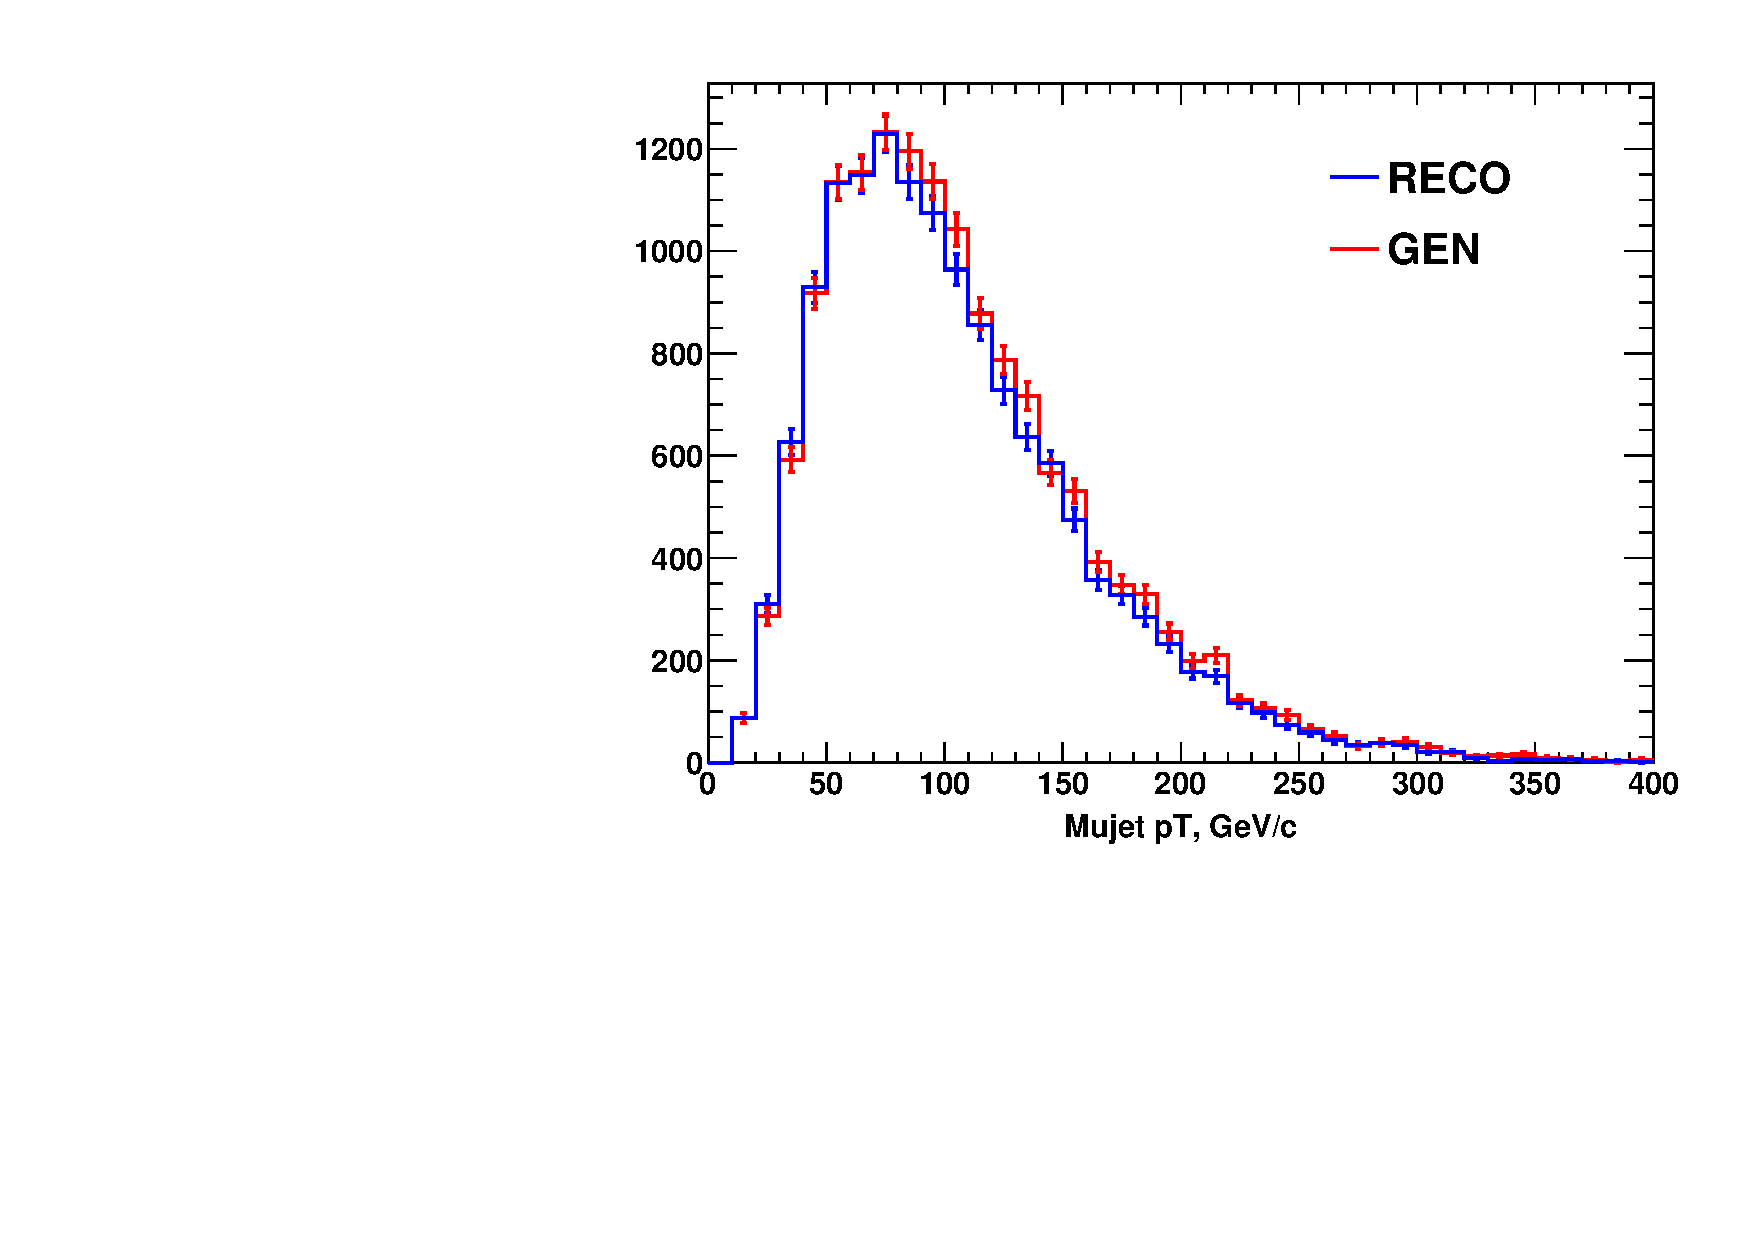
\includegraphics[width=0.5\linewidth]{PLOTS/validation_mujet_pt.pdf} &
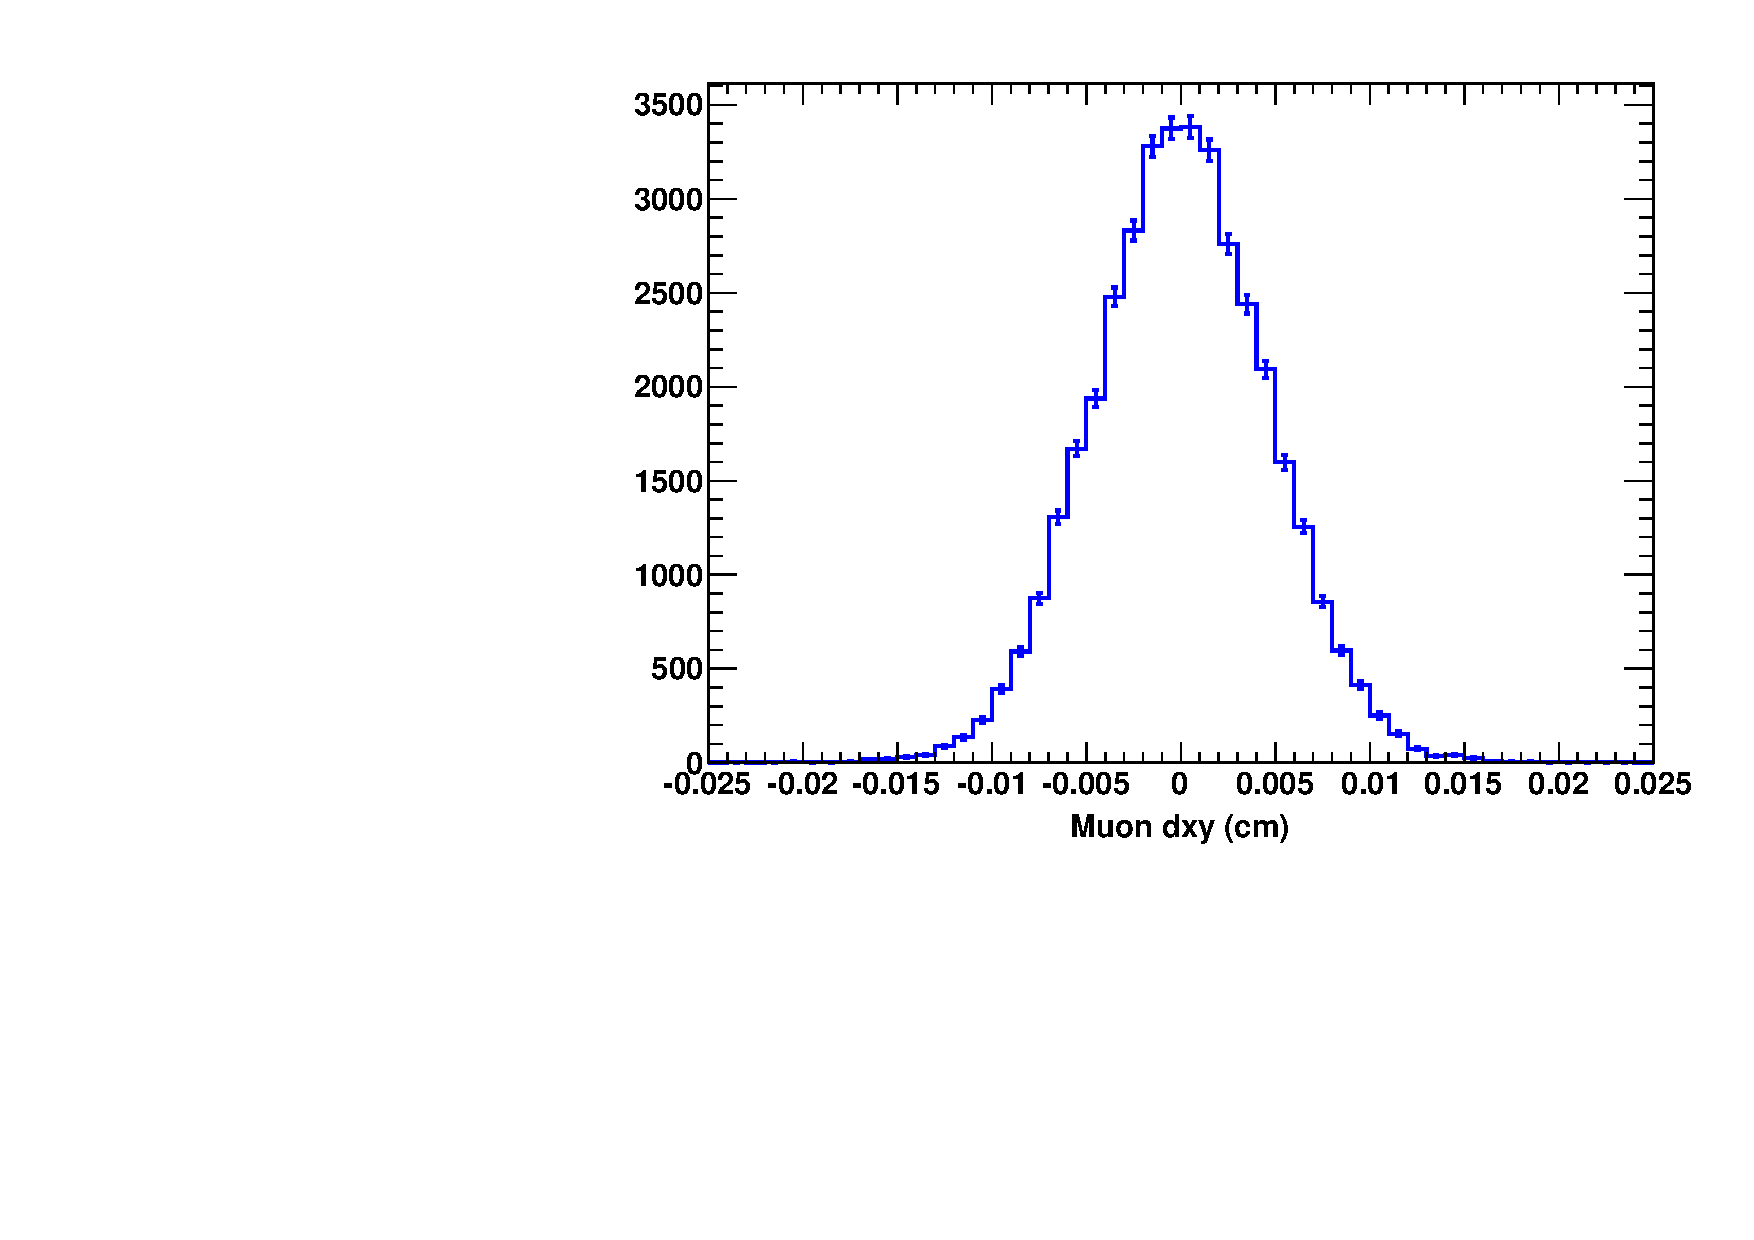
\includegraphics[width=0.5\linewidth]{PLOTS/validation_muon_dxy.pdf} \\
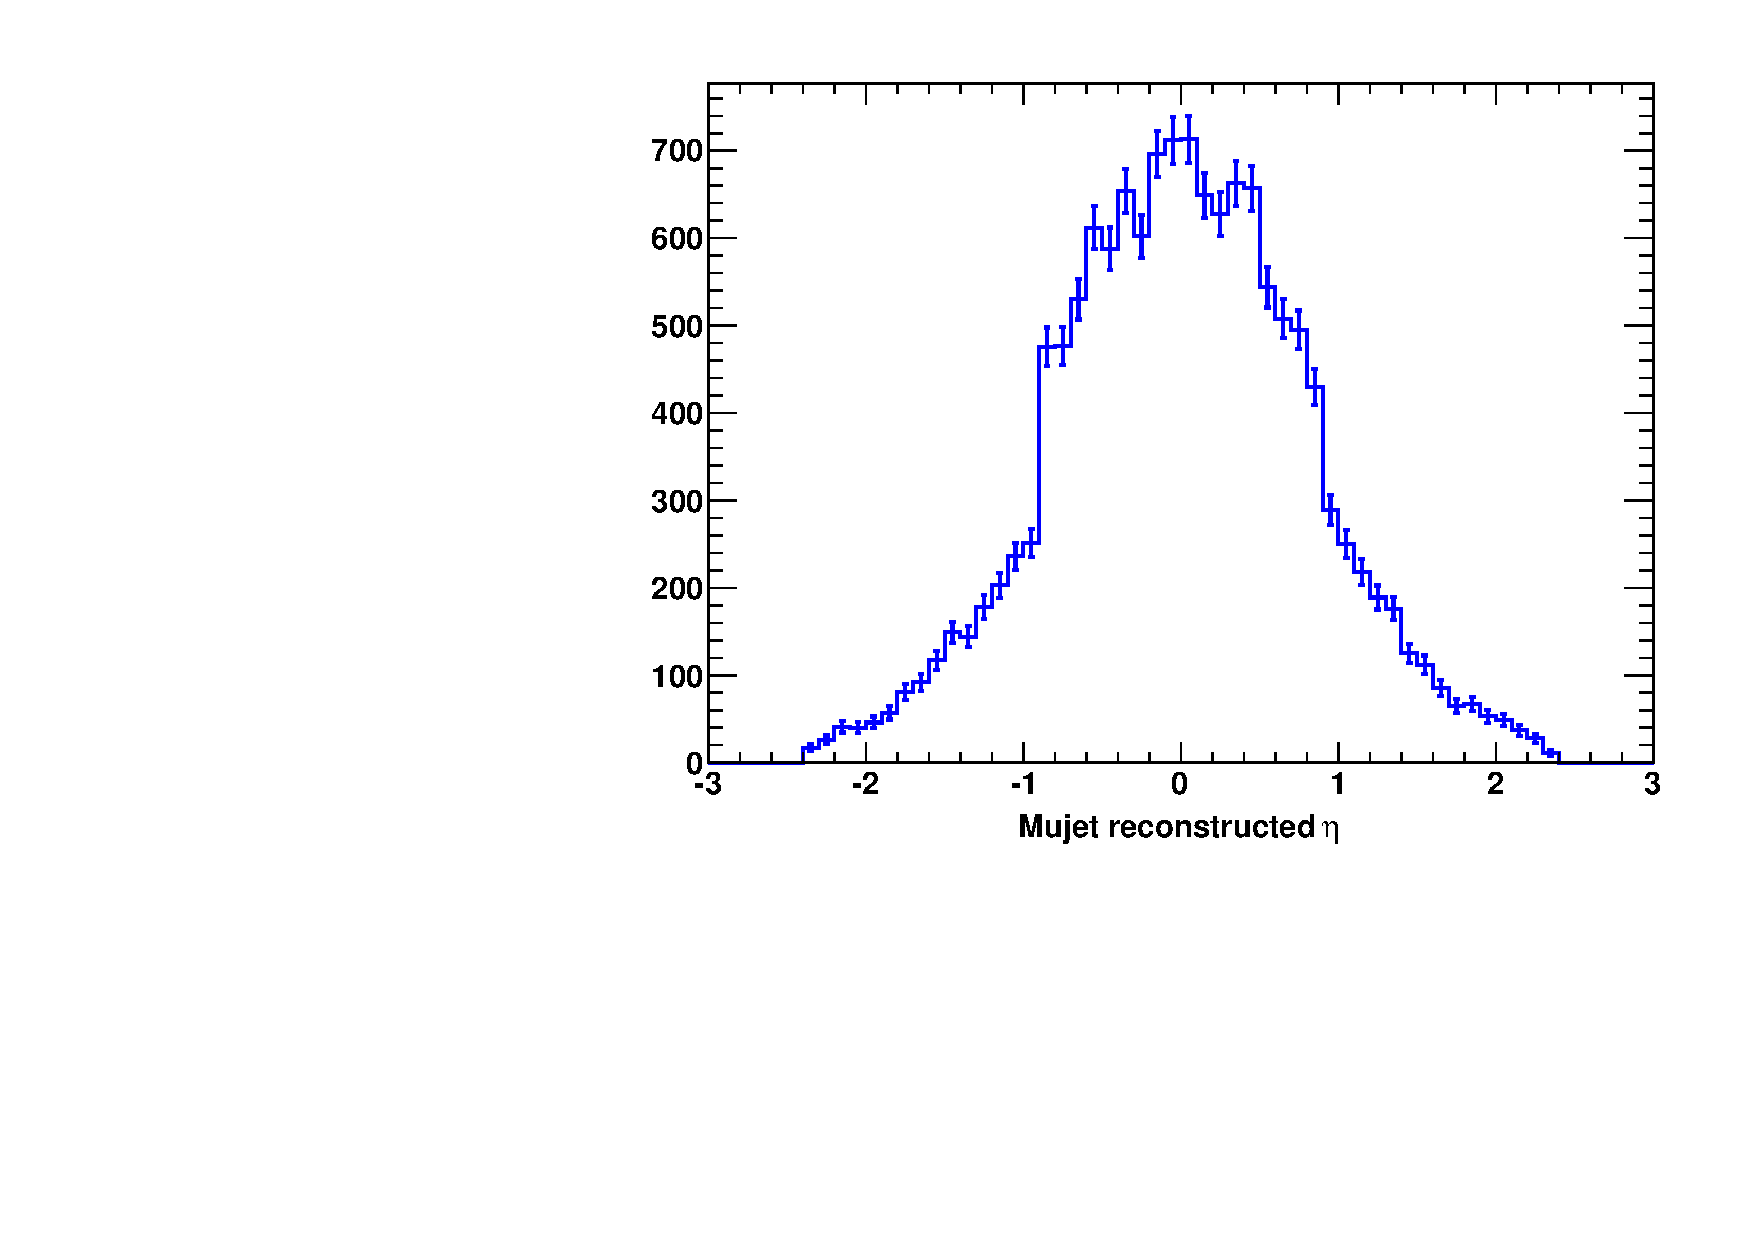
\includegraphics[width=0.5\linewidth]{PLOTS/validation_mujet_eta.pdf} &
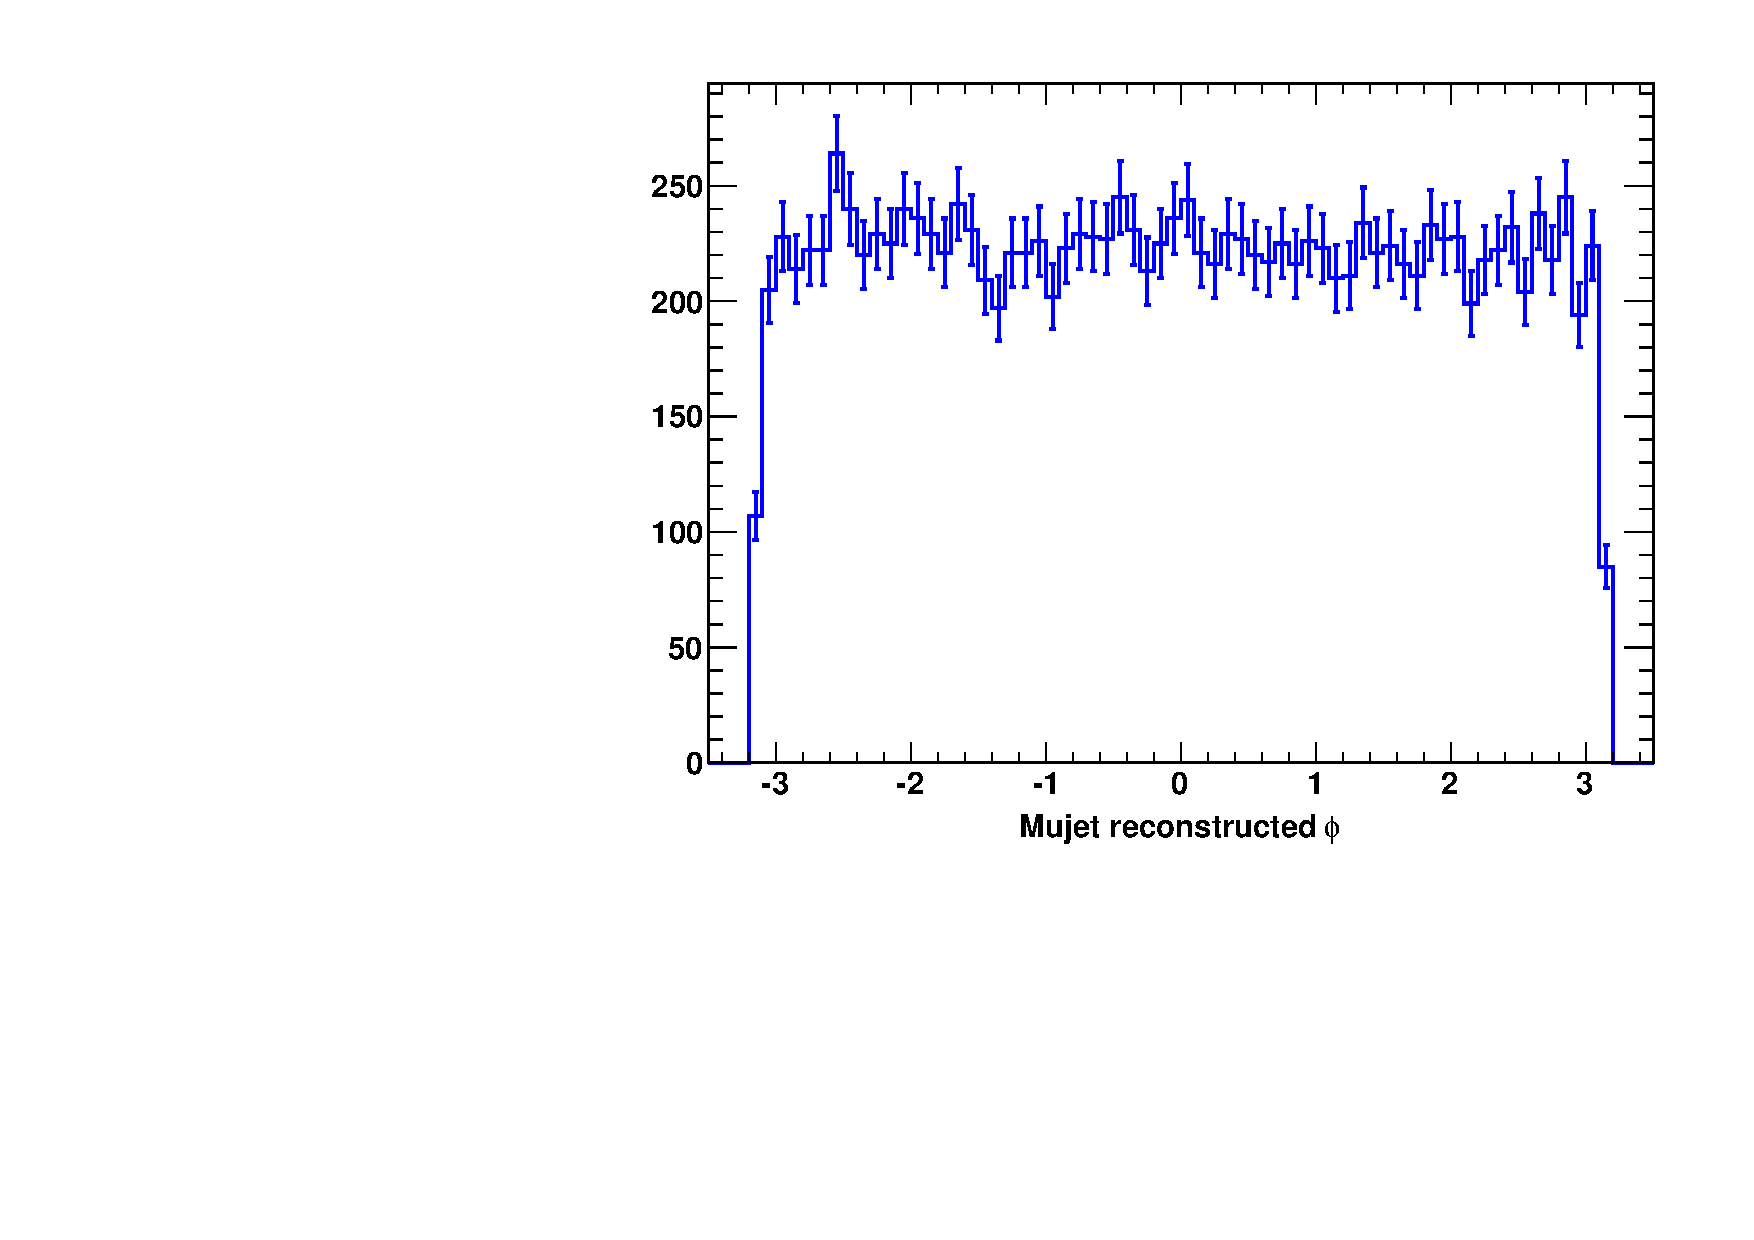
\includegraphics[width=0.5\linewidth]{PLOTS/validation_mujet_phi.pdf}\\
\end{tabular}
\caption{ Basic validation plots of 7 TEV Monte Carlo sample for SUSY with Extra-$\mathcal{U}(1)_{\mbox{\scriptsize dark}}$ model made with the satisfied requirement of a minimal acceptance.  \label{fig:signal_MC_validation_plots}}
\end{figure}

\section{Tracker efficiency study}
\label{sec:tracker_efficiency_study}

This appendix contains a detailed response to the question: Is signal
efficiency affected by interference between muons in the tracker,
possibly in a way that is not well-modeled by Monte Carlo?

\subsection{Dominant efficiency systematic}

Tha dominant efficiency systematic for nearby muons (inverse boost
$1/\gamma \lesssim 0.3$) is from confusion of segments from different
muons in the muon system.  The uncertainty in this inefficiency is
quantified in Fig.~\ref{fig:recoefficiency}: there is a 2\% difference
between crossing and non-crossing muons for leading $p_T >
15$~GeV/$c$, averaged uniformly in $\eta$, and 6\% at the $|\eta| =
2.4$ extreme.  (Definitions and supporting information are in
Appendix~A.)  The cause of the inefficiency is due to incorrectly
assigned segments: every muon track in the analysis is required to
match at least two {\it unique} segments, and if muon $A$ takes muon
$B$'s segments while muon $B$ does not match to muon $A$'s, then muon
$B$ would fail to be identified.  Distances between extrapolated
tracks and muon segments are typically 1--10~cm due to multiple
scattering between the tracker and the muon system, so segments may
even be confused for opening angles as large as 0.3~rad.  The effect
is larger in the endcap because large entrance angles in the magnetic
field bending plane help to distinguish muons in the barrel.

Track-finding efficiencies are much higher than muon-identification
efficiencies: $\sim$99.8\% for $p_T > 5$~GeV/$c$, $|\eta| < 2.4$
tracks compared with $\sim$97\% for muons with the same kinematics.
Since there are no road-broadening effects in the tracker that are
comparable to the multiple scattering in the CMS magnet return yoke,
tracks must be much closer together to suffer inefficiencies in the
tracker alone.  In this document, I will explicitly quantify this
effect with Monte Carlo and information
from \cite{:2009dv,:2009vs,Khachatryan:2010pw}.

I will also compare data and Monte Carlo distributions of the
$\phi(1020)$ resonance, which allows us to test the simulation with
$0.05 < \Delta R < 0.15$ opening angles.

\subsection{CMS track reconstruction procedure}
\label{sec:trackertrackeff1}

The CMS track reconstruction proceeds in five iterations, though the
last three are designed for $p_T < 0.9$~GeV/$c$ and displaced tracks
(low pixel efficiency).  The first two iterations search for
continuations of pairs and triplets of pixel clusters, and only if
clusters can be unambiguously associated with a track (``highPurity'')
are they removed from the list of clusters available in subsequent
iterations.  Tracks found in the same iteration can share up to 50\%
of their clusters.  Clusters may be interpreted differently as hits on
different tracks, due to track-dependent corrections, but inclusion of
a cluster on one track does not automatically disqualify it from
another.

\subsection{Criteria for 50\% overlap}
\label{sec:trackertrackeff2}

To produce tracks that overlap through $\sim$50\% of the tracker, two
oppositely signed muons would need to have very high momentum.  To
estimate this momentum, we use the following facts:
\begin{itemize}
\item pixel channels are 100--150~$\mu$m wide (assume 100),
\item TOB strips are about three times as wide (assume 300),
\item clusters are 1.5--2 channels wide for high-$p_T$ tracks.
\end{itemize}
The first two facts come from a conversation with Kevin Burkett, the
last comes from Fig.~8 and 11 of \cite{:2009dv,:2009vs},
reproduced in Fig.~\ref{fig:cluster_size}.  Cluster size depends
primarily on path length through the silicon, with a near-minimum for
high-$p_T$ tracks (near-minimal because of the magnetic field).

\begin{figure}
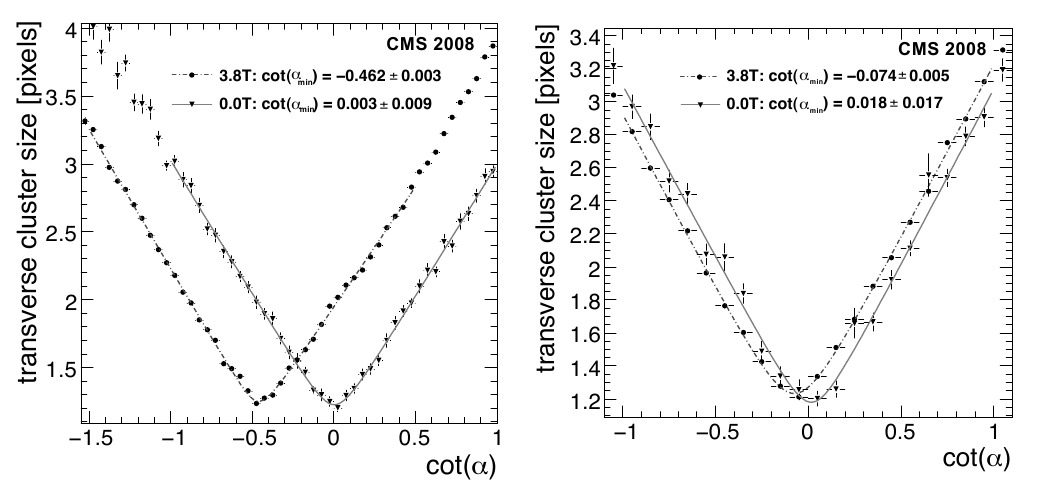
\includegraphics[width=0.6\linewidth]{PLOTS/writeup/pixel_clusters.png}
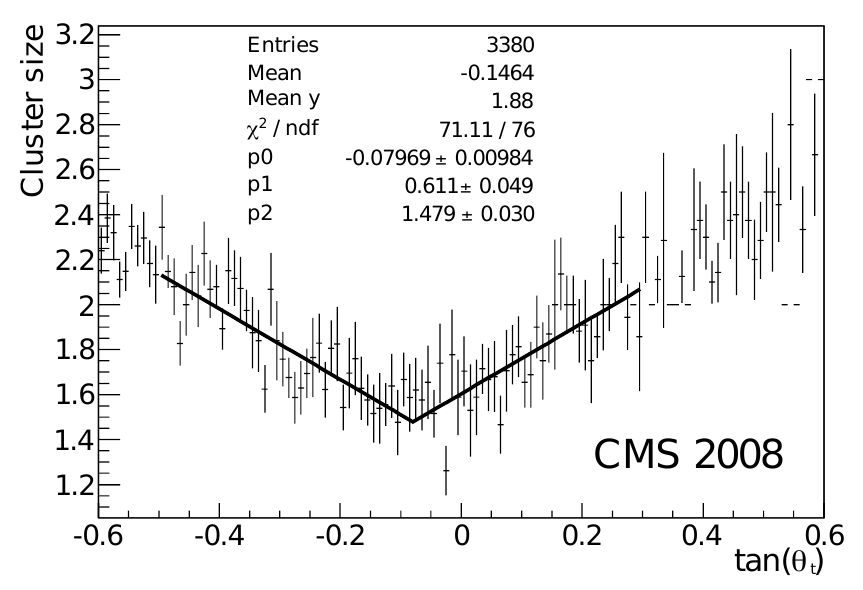
\includegraphics[width=0.4\linewidth]{PLOTS/writeup/strip_clusters.png}

\caption{Cluster size versus entrance angle in the pixel barrel
  (left), pixel endcap (middle), with and without magnetic field, and
  TOB layer 4 (right).  High-$p_T$ tracks have minimal entrance
  angle.  Reproduced from \cite{:2009dv,:2009vs}. \label{fig:cluster_size}}
\end{figure}

\begin{figure}[p]
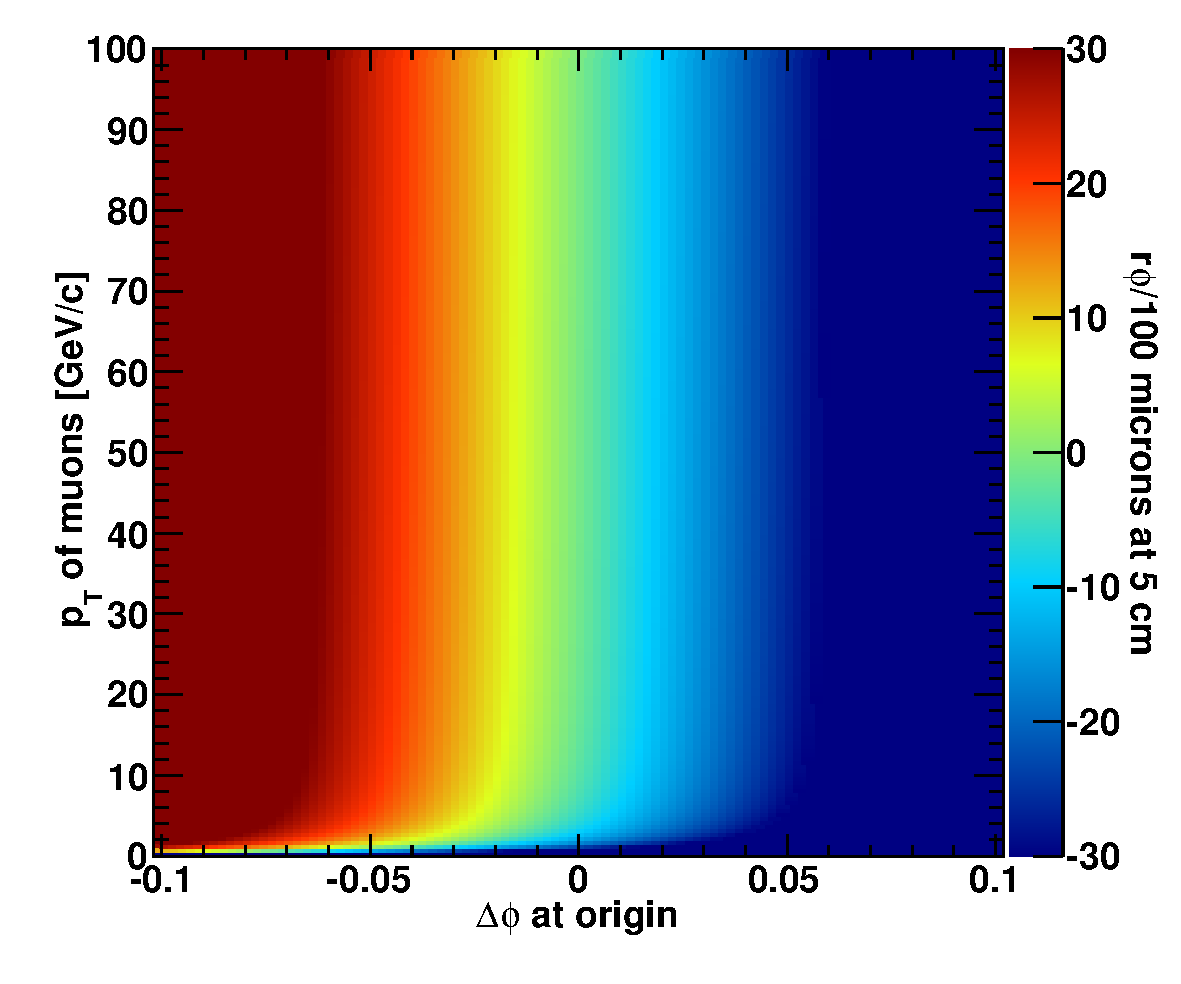
\includegraphics[width=0.5\linewidth]{PLOTS/writeup/separation_at_5cm.pdf}
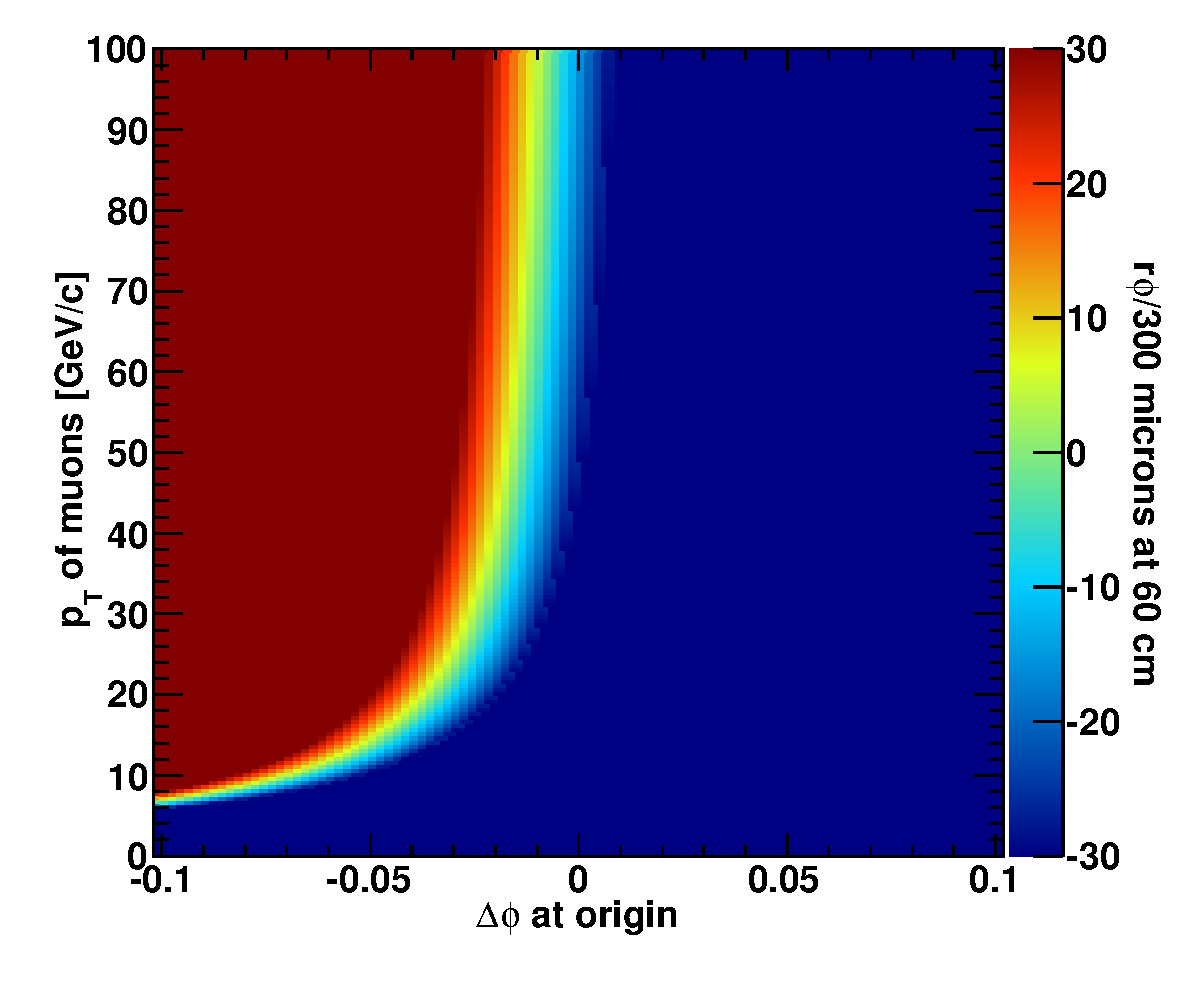
\includegraphics[width=0.5\linewidth]{PLOTS/writeup/separation_at_60cm.pdf}

\caption{Separation of two muon trajectories at the first pixel layer,
  5~cm from the beamline (left), and the first TOB layer, 60~cm from
  the beamline (right).  The color scale is the $r\phi$ distance
  between the muon trajectories on a cylinder of the given radius,
  measured in units of channel widths, taking 100~$\mu$m for the pixel
  and 300~$\mu$m for the TOB.  Green is zero separation; red and blue
  are 30 channels apart.  The $r\phi$ separation asymptotically
  approaches a constant multiple of $\Delta \phi$ at the origin for
  high-$p_T$ muons (both muons have the same
  $p_T$ in this simulation). \label{fig:separation}}
\end{figure}

\begin{figure}[p]
\begin{center}
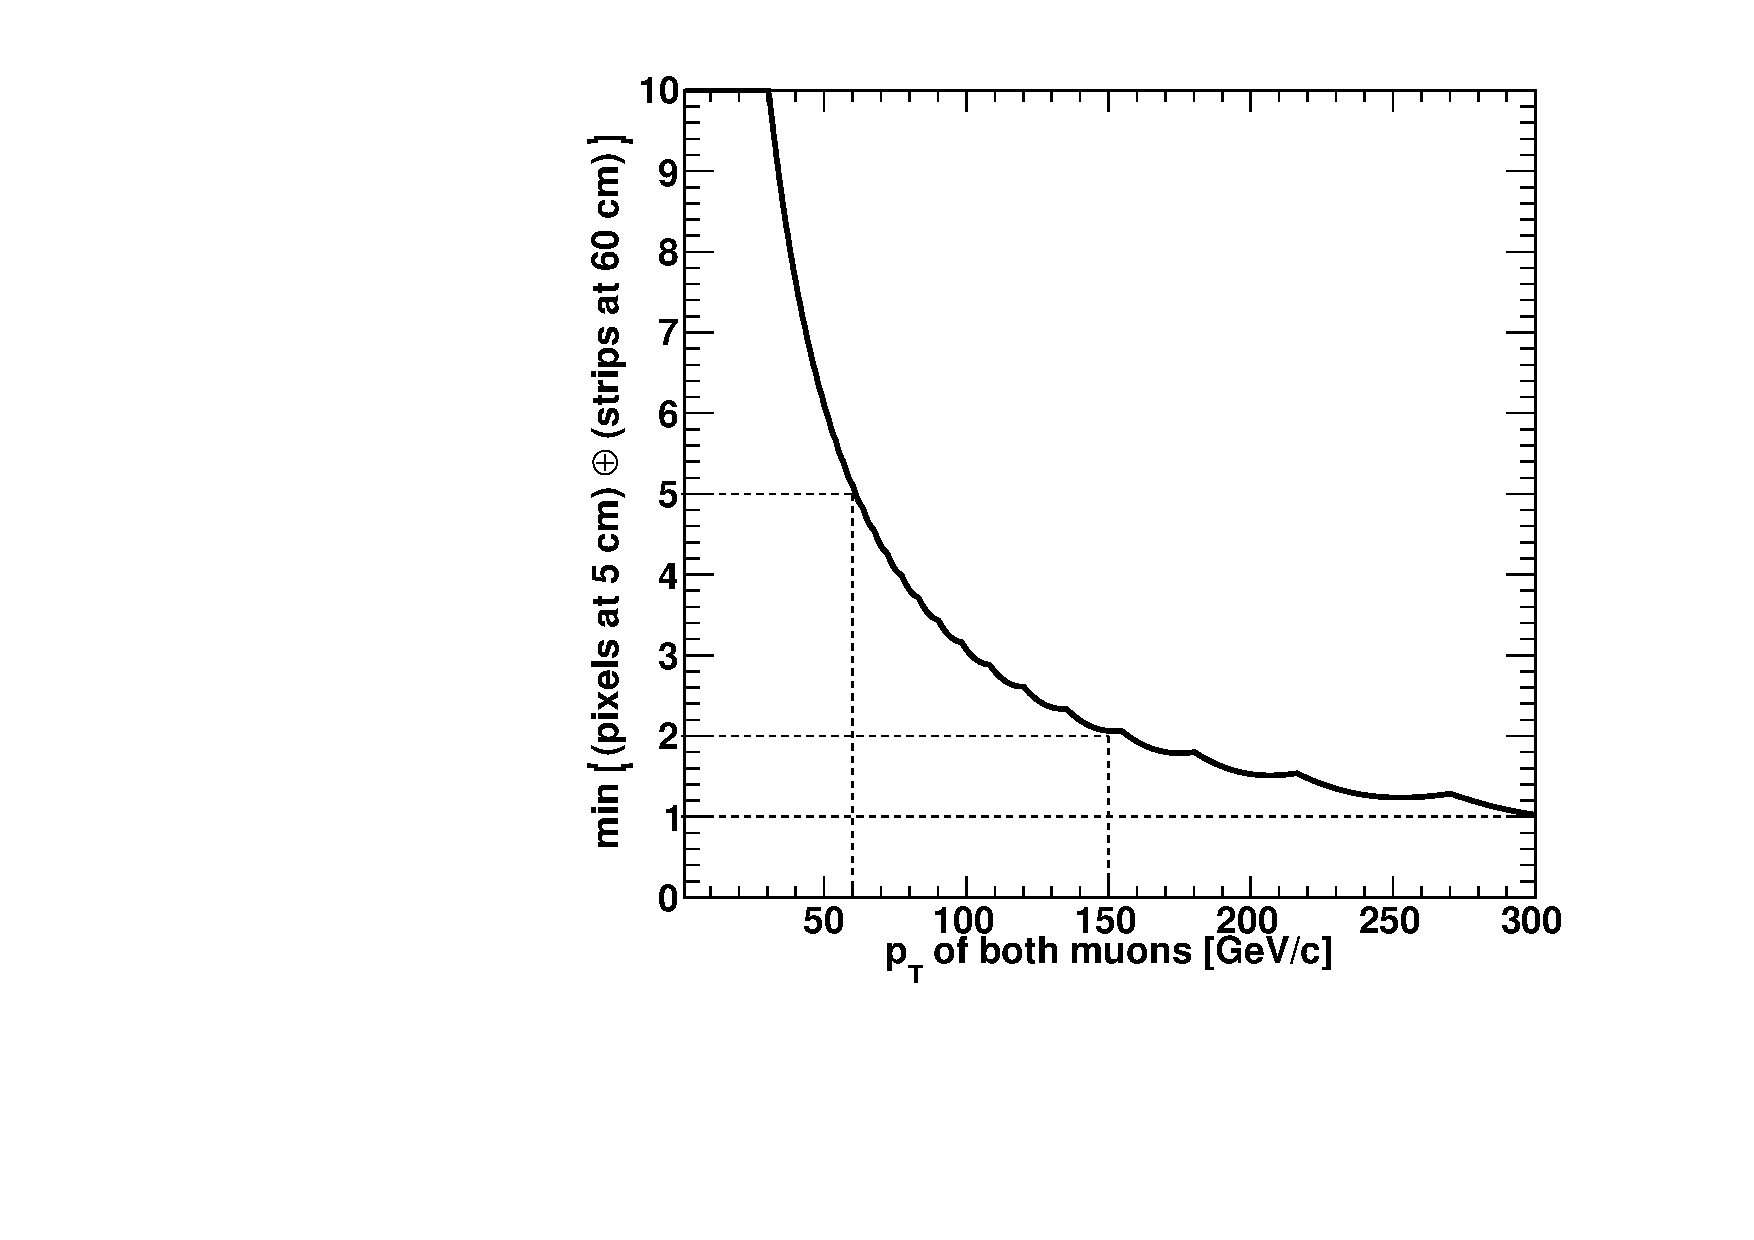
\includegraphics[width=0.5\linewidth]{PLOTS/writeup/separation_minimum.pdf}
\end{center}

\caption{Minimum separation in {\it both} the pixel detector at a
  radius of 5~cm {\it and} the TOB at a radius of 60~cm.  The vertical axis
  is the minimum $r\phi$ separation in pixel channel widths, added in
  quadrature with the minimum $r\phi$ separation in TOB channel
  widths, minimized over possible values of $\Delta \phi$ at the
  origin.  For two muons to be separated by $\sim$1 channel width in
  the pixel {\it and} TOB, both muons would need about $p_T \approx
  300$~GeV/$c$. \label{fig:separation2}}
\end{figure}

Figures~\ref{fig:separation} and \ref{fig:separation2} quantify the
degree of separation at two distances from the beamline: 5~cm (first
pixel layer) and 60~cm (first TOB layer, about 50\% through the
tracker).  Two trajectories were propagated from the origin to 5 and
60~cm cylinders using the appropriate CMSSW propagator for a variety
of $\Delta \phi$ opening angles at the origin and initial $p_T$ of
both trajectories (both momenta were equal, with $\eta = 0$).  For a
$\sim$5~channel width separation at both radii, both muons would need
$p_T > 60$~GeV/$c$, for $\sim$2 channel widths, both muons would need
$p_T > 150$~GeV/$c$, and for $\sim$1 channel width, both muons would
need $p_T > 300$~GeV/$c$.

\subsection{Observing track interference in pair-gun MC}
\label{sec:trackertrackeff3}

To search for the onset of an inefficiency due to nearby tracks in the
tracker, I plotted efficiency versus $\Delta R$ using our pair-gun MC.
The pair-gun MC is a full CMSSW simulation of two opposite-sign muons
with uniformly random pair momentum ($0 < p_T^{\mu\mu} <
100$~GeV/$c$), mass ($2m_\mu < m < 6$~GeV/$c^2$), pseudorapidity
($-2.5 < \eta^{\mu\mu} < 2.5$), and azimuthal angle ($-\pi <
\phi^{\mu\mu} < \pi$).  Each pair of muons is reconstructed three
times: once with the $\mu^+$ as the only particle in the event, once
with the $\mu^-$ as the only particle in the event, and once with both
$\mu^+$ and $\mu^-$ in the same event.  This allows us to study
efficiency losses due to interference separately from single-particle
efficiency.

With these tools, we can define ``interference efficiency'' in the
following way:
\begin{equation}
P(\mu^+\mu^- | \mu^+\mbox{ and }\mu^-) = \frac{\mbox{both muons
  reconstructed in the same event and separately}}{\mbox{both muons
    reconstructed separately}}
\end{equation}
with additional generator-level requirements of $p_T > 5$~GeV/$c$
and $|\eta| < 2.4$ for both numerator and denominator.
``Reconstructed'' means that the reconstructed track exists with $\ge
8$ hits and $\chi^2/N_{\mbox{\scriptsize dof}} < 4$, though these quality cuts have
negligible impact on the final result.  The probability of
reconstructing both muons separately, given kinematical acceptance, is
99.6\%.

Figure~\ref{fig:doubleeff} presents this interference efficiency as a
function of $\Delta R$, where an 8\% dip is visible for $\Delta R <
0.01$.  This dip is correlated with high momentum (same figure),
suggesting that it is related to track overlap.  For context, we show
the mass distribution of muon pairs with $\Delta R < 0.01$ in this
sample in Fig.~\ref{fig:doubleeff_mass}.  The 100~GeV/$c$ upper limit
in momentum implies only mass $<$ 0.5~GeV/$c^2$ pairs have such a
small opening angle.  For a 1~GeV/$c^2$ boson, the onset of the effect
would be at higher momenta.

\begin{figure}
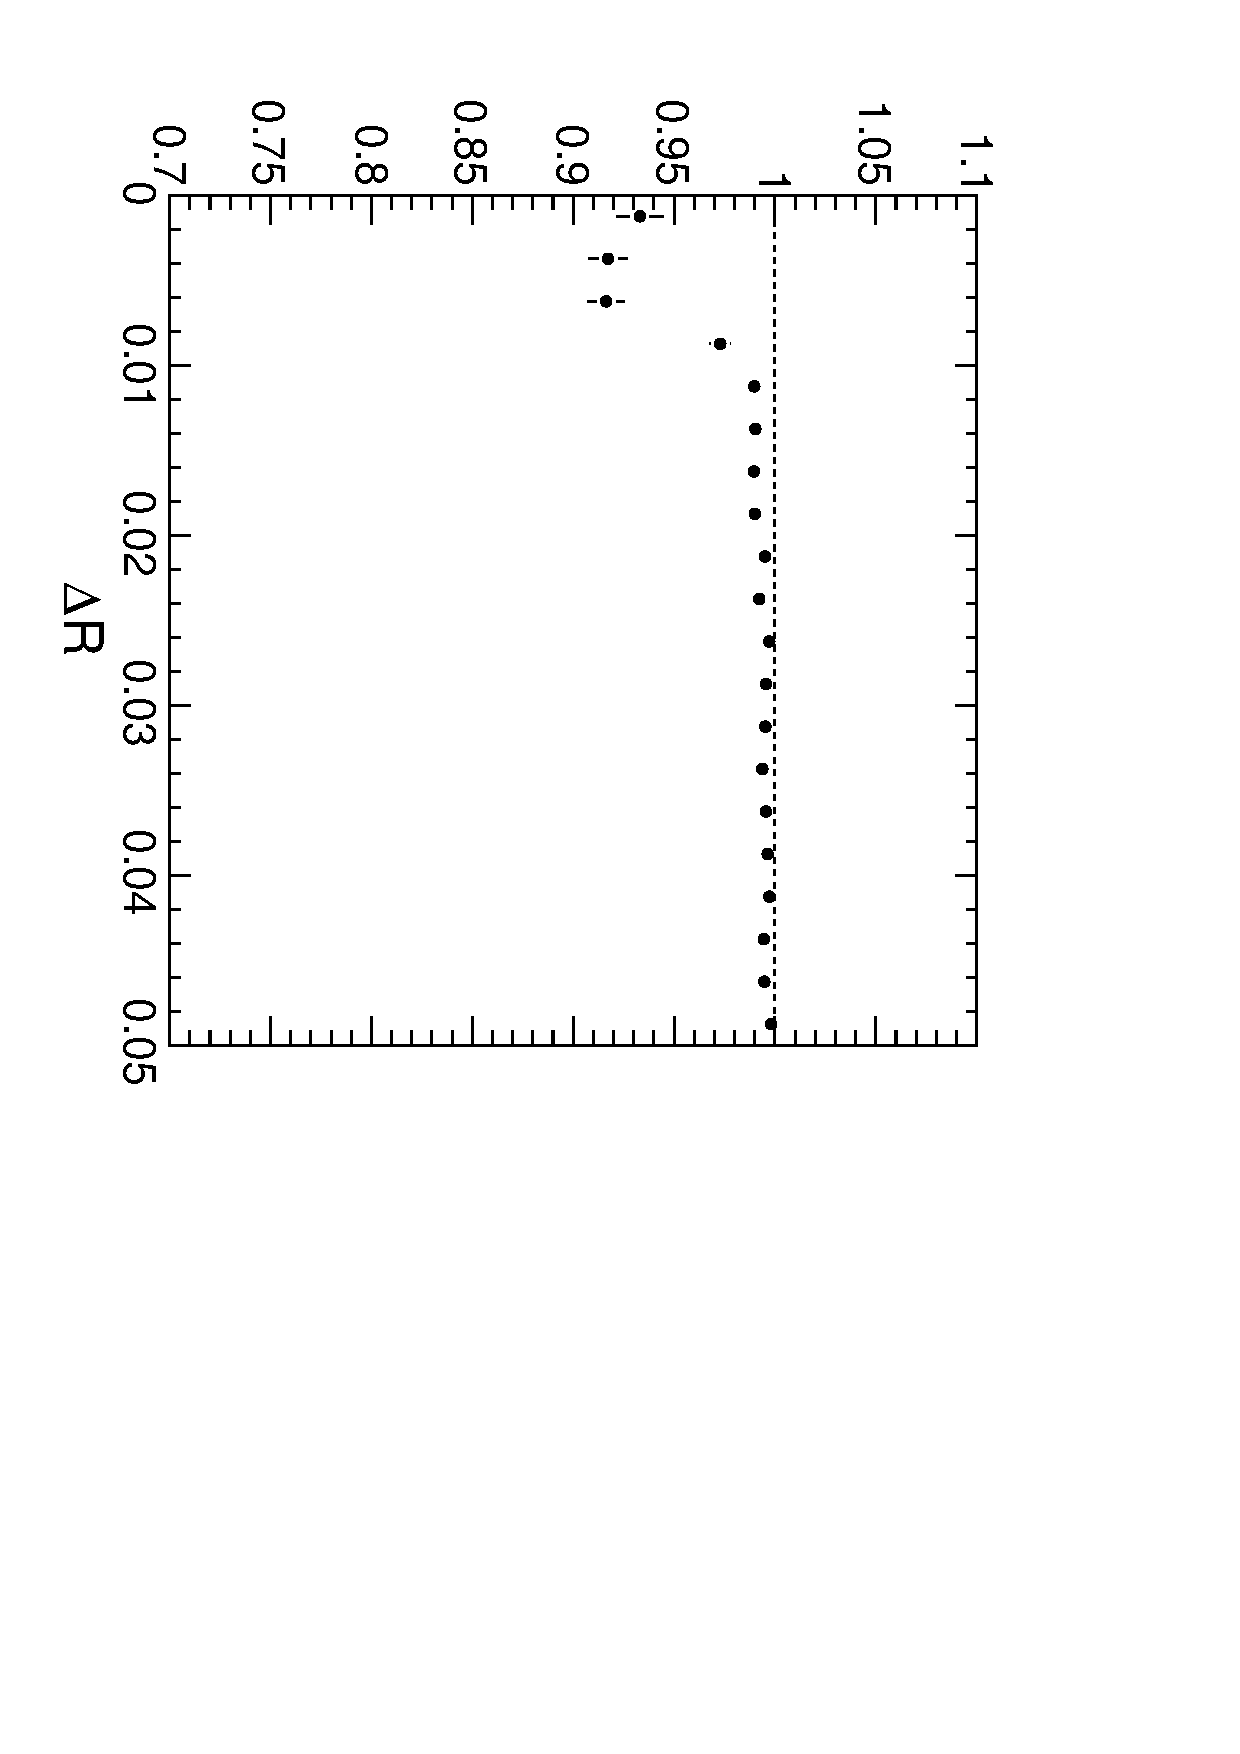
\includegraphics[height=0.5\linewidth, angle=90]{PLOTS/writeup/doubleeff_deltar.pdf}
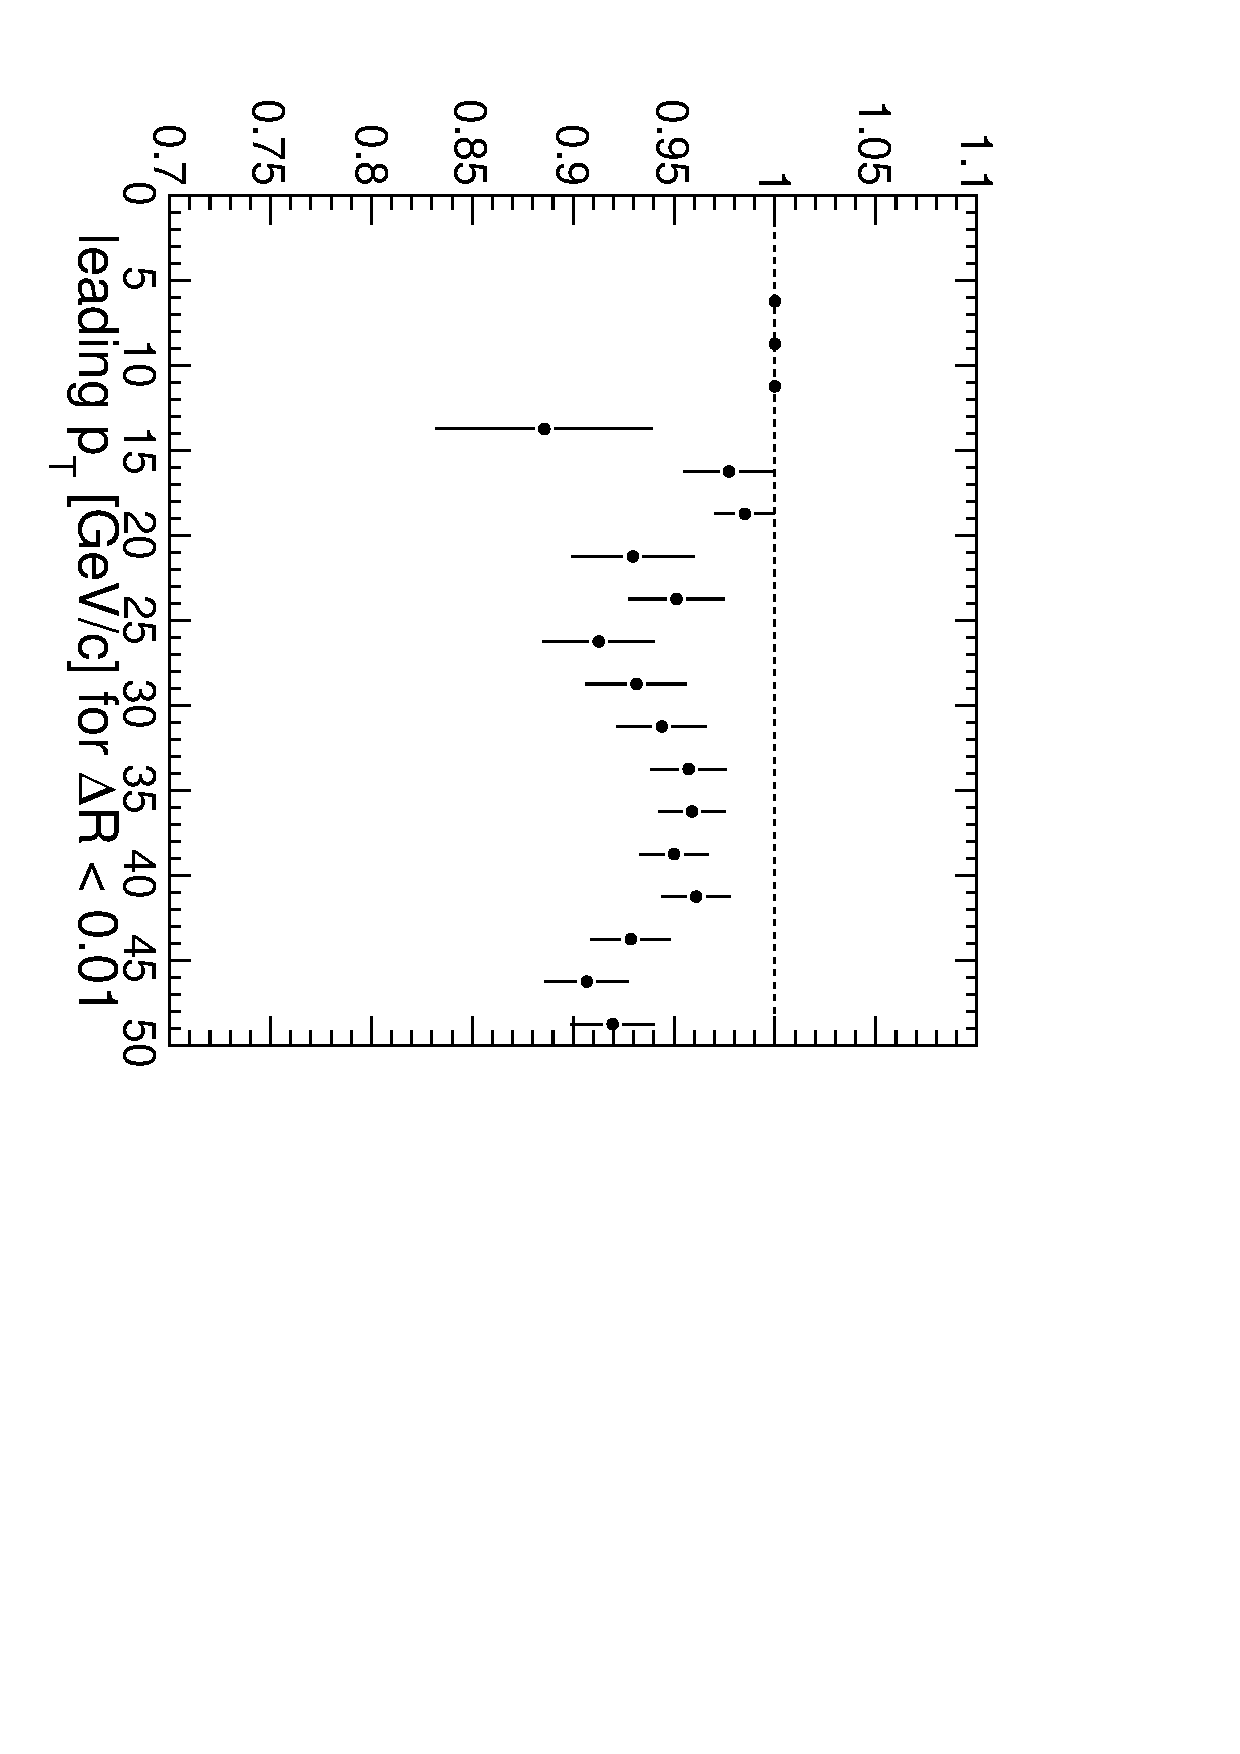
\includegraphics[height=0.5\linewidth, angle=90]{PLOTS/writeup/doubleeff_leadpt.pdf}

\caption{Left: $P(\mu^+\mu^- | \mu^+\mbox{ and }\mu^-)$ for track cuts
  (see text) versus $\Delta R$.  Right: the same quantity versus
  leading muon $p_T$ for $\Delta R < 0.01$, showing that the effect
  prefers high momenta. \label{fig:doubleeff}}
\end{figure}

\begin{figure}
\begin{center}
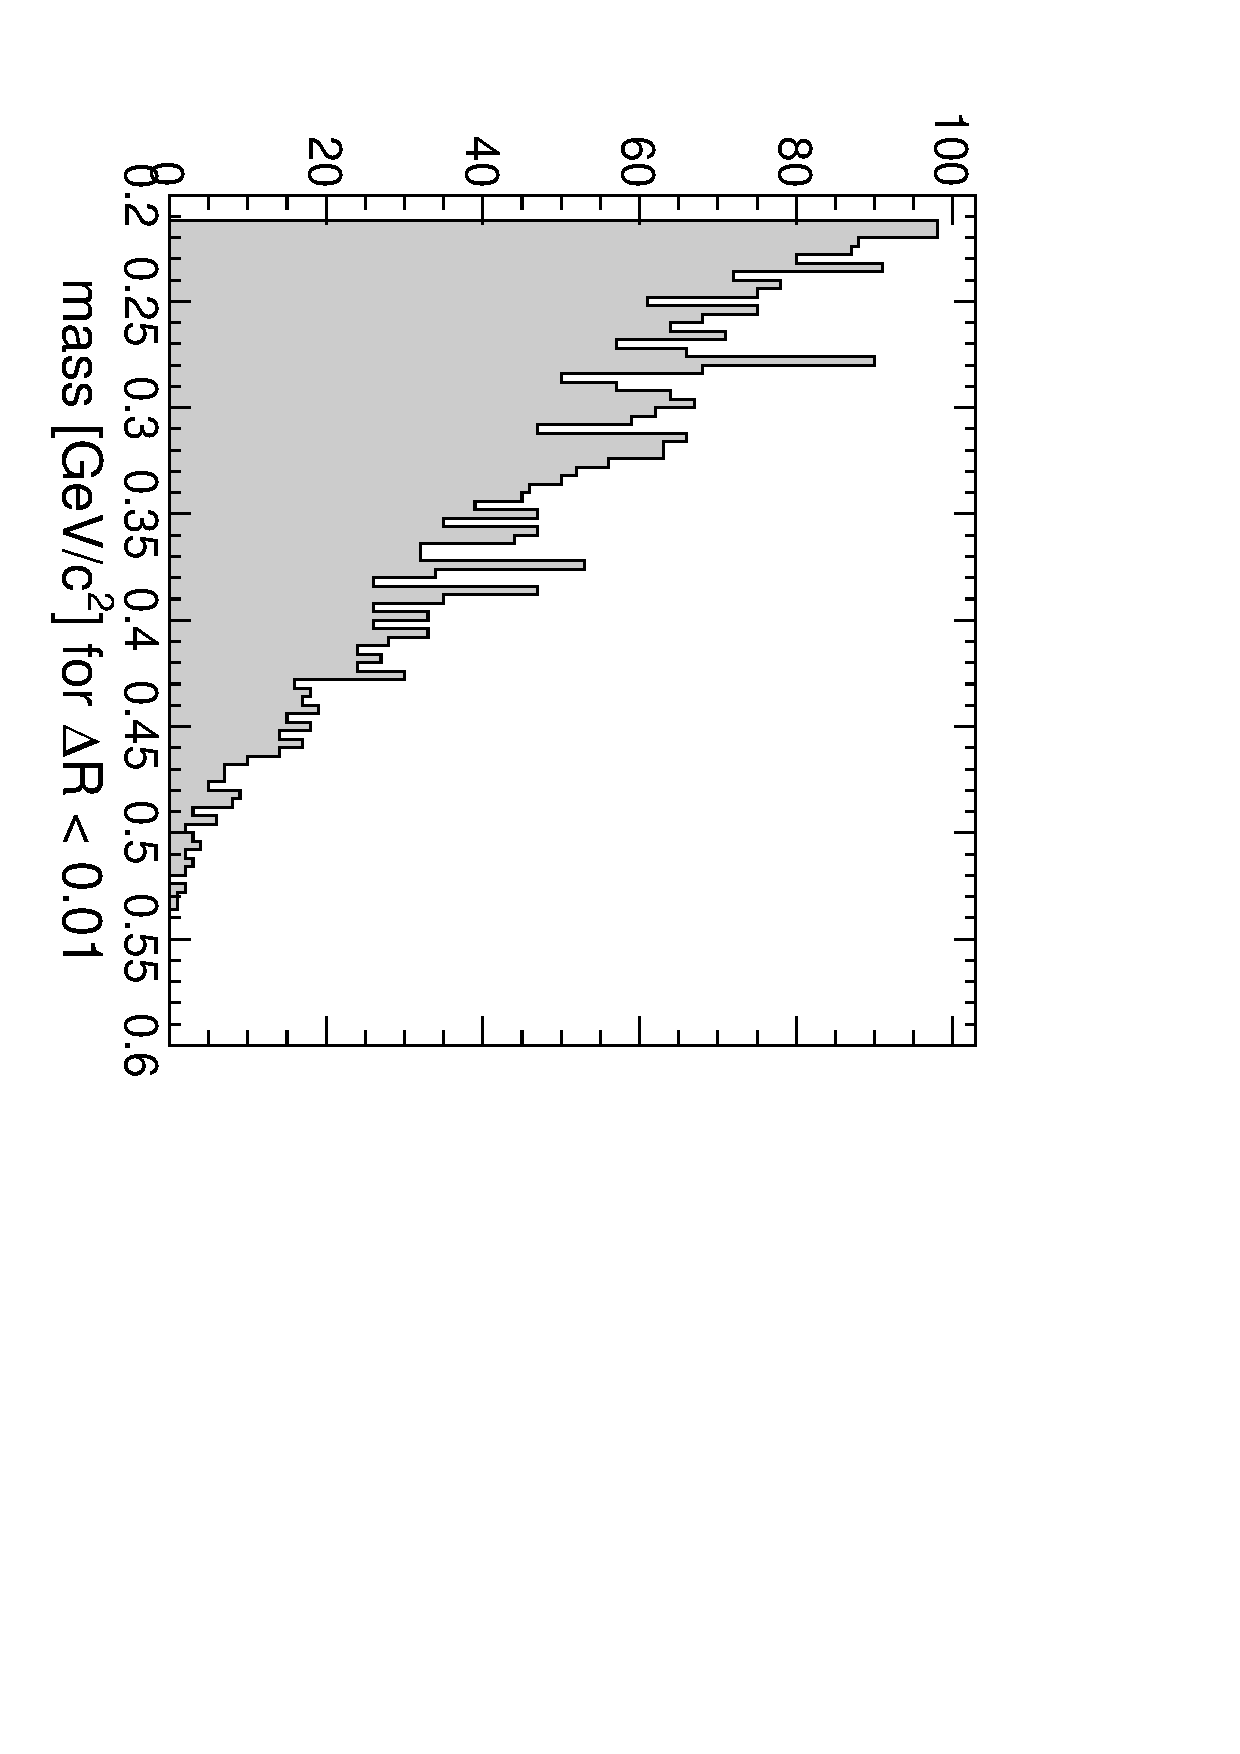
\includegraphics[height=0.5\linewidth, angle=90]{PLOTS/writeup/doubleeff_mass.pdf}
\end{center}

\caption{Values of muon pair mass consistent with $\Delta R < 0.01$ in
  this simulation, for context. \label{fig:doubleeff_mass}}
\end{figure}

The same study can be performed for the full muon cuts, that is,
adding the requirement that the track is reconstructed as a
TrackerMuon with $\ge 2$ arbitrated muon segments.  This is presented
in Fig.~\ref{fig:doubleeff_muon}.  The interference efficiency for the
full muon cuts has the same shape as a function of $\Delta R$, though
a lower plateau for $\Delta R \gg 0.01$.  This is the effect of
the muons crossing the muon system (discussed in the analysis note),
which is not a strict fuction of $\Delta R$ at the origin.

\begin{figure}
\includegraphics[height=0.5\linewidth, angle=90]{PLOTS/writeup/doubleeff_deltar_muon.pdf}
\includegraphics[height=0.5\linewidth, angle=90]{PLOTS/writeup/doubleeff_leadpt_muon.pdf}

\caption{Left: $P(\mu^+\mu^- | \mu^+\mbox{ and }\mu^-)$ for muon cuts
  versus $\Delta R$.  Right: the same quantity versus leading muon
  $p_T$ for $\Delta R < 0.01$, showing that the effect prefers high
  momenta. \label{fig:doubleeff_muon}}
\end{figure}

\subsection{Data/MC comparisons for tracking}

Reference~\cite{Khachatryan:2010pw} presents a detailed overview of
the status of the tracking simulation with early collisions.  The
simulation is shown to reproduce the shapes of signal responses (see
Fig.~\ref{fig:cluster_charge}, copied from the paper) and many
high-level tracking quantities.  Figure~\ref{fig:ourcuts} shows the
number of hits and $\chi^2/N_{\mbox{\scriptsize dof}}$ distributions from this paper,
which are relevant to our analysis as track quality cuts.  The
distributions in the early LHC paper represent low-$p_T$ hadrons,
rather than $p_T > 5$~GeV/$c$ muons, though.

\begin{figure}
\includegraphics[width=\linewidth]{PLOTS/writeup/cluster_charge.png}

\caption{Figure reproduced from \cite{Khachatryan:2010pw}. \label{fig:cluster_charge}}
\end{figure}

\begin{figure}
\includegraphics[width=0.5\linewidth]{PLOTS/writeup/number_of_hits.png}
\includegraphics[width=0.5\linewidth]{PLOTS/writeup/normalized_chi2.png}

\caption{Two figures from the early LHC tracking paper relevant to our
  analysis: blue lines indicate our cuts.  These distributions have
  different shapes for our $p_T > 5$~GeV/$c$
  tracks. \label{fig:ourcuts}}
\end{figure}

One may argue that the tracking simulation may be trusted if it
reproduces all low-level signals and has a realistic alignment, since
our analysis signal only differs in geometry, and all geometry and
algorithms are the same for data and Monte Carlo.  This can be
partially tested with studies of the $\phi(1020)$ resonance.

\subsection{Study of the $\phi(1020)$ resonance}

The $\phi(1020)$ resonance provides a standard candle of low-mass,
moderately high-momentum dimuons with which to test the level of
data/MC agreement.  It corresponds to a moderately low range of
opening angles $0.05 < \Delta R < 0.15$, though not low enough to
sample the $\Delta R < 0.01$ tracker inefficiency.  It is the
lowest-mass Standard Model narrow resonance found in both data and
Monte Carlo ($\omega(782) \to \mu\mu$ is missing from the Pythia~6
decay tables), and it is in the middle of the target mass range of our
analysis, though lower than our target momentum range.

Figure~\ref{fig:phi_mass} presents the invariant mass distribution
near the $\phi(1020)$ peak, indicating the signal region ($|m -
m_\phi| < 0.025$~GeV/$c^2$), the sidebands ($0.050 < |m -
m_\phi| < 0.075$~GeV/$c^2$), and a pure $\phi(1020)$ Monte Carlo
simulation.  The $\phi(1020)$ simulation is a subset of
InclusiveMu5\_Pt30 (muons from Pythia 6 QCD): dimuons selected at
generator level to have $\phi(1020)$ as their parent.

\begin{figure}
\begin{center}
\includegraphics[width=0.75\linewidth]{PLOTS/writeup/phi_mass.pdf}
\end{center}

\caption{Basic distribution of the $\phi(1020)$ study: dimuon
  invariant mass distribution of data (dashed line, colored in
  sections) with the signal region indicated by yellow, the sidebands
  indicated by blue, overlaid with a pure $\phi(1020)$ MC simulation
  (unscaled). \label{fig:phi_mass}}
\end{figure}

The $\phi(1020)$ events in Monte Carlo are all prompt and in jets,
while the data has a displaced component and an isolated component.
For a more appropriate comparison, I applied the following cuts:
\begin{itemize}
\item distance between the dimuon vertex and the closest primary
  vertex in $z$ must be less than 1~mm ($L_{xy} < 1$~mm);
\item the sum of track $p_T$ for $p_T > 1.5$~GeV/$c$ in a $\Delta R <
  0.4$ cone around the dimuon axis must be greater than 3~GeV/$c$
  ($Iso > 3$~GeV/$c$);
\item exactly two reconstructed muons per event;
\item apply $|m - m_\phi| < 0.025$~GeV/$c^2$ to Monte Carlo as well as
  the signal;
\item at least one muon must have $p_T > 10$~GeV/$c$.
\end{itemize}
The data were collected using any single or double-muon trigger that
was available.  Prescales changed during the run, but HLT\_Mu9 and
HLT\_Mu11 were prescaled late in the year--- the requirement of $p_T >
10$~GeV/$c$ is a compromise between strict correctness (our analysis
uses only $p_T > 15$~GeV/$c$) and the need to maximize the size of the
dataset for statistically meaningful comparisions.
Figure~\ref{fig:phi_muon12pt} shows sideband-subtracted $\phi(1020)$
data overlaid by normalized Monte Carlo of the highest and
lowest-$p_T$ muon in each event.  The data and Monte Carlo $p_T$
spectra are consistent: there is no evidence of trigger prescale
thresholds in the spectrum.  Figure~\ref{fig:phi_other} presents the
$\Delta R$, $\eta$, $Iso$, and $L_{xy}$ distributions (with all cuts
applied).

\begin{figure}
\includegraphics[width=0.5\linewidth]{PLOTS/writeup/phi_muon1pt.pdf}
\includegraphics[width=0.5\linewidth]{PLOTS/writeup/phi_muon2pt.pdf}

\caption{Sideband-subtracted muon momentum distributions overlaid by
  Monte Carlo (normalized to equal number of events). \label{fig:phi_muon12pt}}
\end{figure}

\begin{figure}
\includegraphics[width=0.5\linewidth]{PLOTS/writeup/phi_dr.pdf}
\includegraphics[width=0.5\linewidth]{PLOTS/writeup/phi_eta.pdf}

\includegraphics[width=0.5\linewidth]{PLOTS/writeup/phi_iso.pdf}
\includegraphics[width=0.5\linewidth]{PLOTS/writeup/phi_lxy.pdf}

\caption{Other distributions relevant for or used to define the
  $\phi(1020)$ sample. \label{fig:phi_other}}
\end{figure}

Figure~\ref{fig:phi_cuts} shows the same sideband-subtracted data
overlaid by normalized Monte Carlo for the distributions used to
define muon quality cuts: number of tracker hits, tracker
$\chi^2/N_{\mbox{\scriptsize dof}}$, and number of arbitrated muon segments.  All cuts
are far from the distributions except the number of segments.  The
number of segments matched to a TrackerMuon track depends on the level
of agreement between tracks propagated from the tracker and muon
segment positions and entrance angles, which are shown in
Fig.~\ref{fig:phi_residuals}.

\begin{figure}
\begin{center}
\includegraphics[width=0.48\linewidth]{PLOTS/writeup/phi_hits.pdf}
\includegraphics[width=0.48\linewidth]{PLOTS/writeup/phi_normchi2.pdf}

\vspace{0.25 cm}
\includegraphics[width=0.48\linewidth]{PLOTS/writeup/phi_matches.pdf}
\end{center}

\caption{Distributions of track quality cuts (top row) and muon
  quality cuts (bottom) with cut thresholds indicated in blue.  All
  cuts have been applied in all distributions. \label{fig:phi_cuts}}
\end{figure}

\begin{figure}
\includegraphics[width=0.5\linewidth]{PLOTS/writeup/phi_st1x.pdf}
\includegraphics[width=0.5\linewidth]{PLOTS/writeup/phi_st1xsig.pdf}

\includegraphics[width=0.5\linewidth]{PLOTS/writeup/phi_st1dxdz.pdf}
\includegraphics[width=0.5\linewidth]{PLOTS/writeup/phi_st1dxdzsig.pdf}

\caption{Distance between propagated track and muon segment in the
  magnetic field bending plane ($x$, top-left), the same normalized by
  uncertainty (top-right), the difference in entrance angle ($dx/dz$,
  bottom-left), and the same normalized by uncertainty (bottom-right).
  These are relevant for determining the number of muon segments
  matched to a TrackerMuon. \label{fig:phi_residuals}}
\end{figure}

The Monte Carlo sample used in this study and all signal samples used
in the main analysis were produced using ideal alignment and
calibration conditions.  The data in this $\phi(1020)$ study is a
combination of Sep17ReReco (2010A) and PromptReco (2010B), unlike the
main analysis, which uses Dec22ReReco.  The only observed discrepancy
between data and Monte Carlo is in the $\chi^2/N_{\mbox{\scriptsize
dof}}$ distribution (Fig.~\ref{fig:phi_cuts} top-right), in which the
Monte Carlo peaks at one but the data peaks lower than one.  This
could be because the tracker alignment uses artificially inflated
Alignment Position Errors (APEs) in PromptReco for safety.  The muon
residuals distributions (Fig.~\ref{fig:phi_residuals}) are completely
insensitive to muon alignment conditions for $\sim$20~GeV/$c$ muon
momenta because of the dominance of multiple scattering in the
propagation.

\subsection{Tracker efficiency conclusions}

Muon segment assignment for muons whose trajectories cross in the muon
system is the dominant efficiency systematic for a wide range of
opening angles.  However, efficiency losses in the tracker could play
a significant role for 150--300~GeV/$c$ muons.  An 8\% loss in
efficiency is observed in pair-gun MC for $\Delta R < 0.01$ muon
pairs, though such a high boost is a special case in our analysis.
The simulation was tested for moderately low opening angles ($0.05 <
\Delta R < 0.15$) using the $\phi(1020)$ resonance, though the region
where the tracker begins to be inefficient for nearby muons is
orthogonal to this or any test using Standard Model resonances.

\section{MuscleFit study}
\label{sec:muscle_fit}

In order to estimate the effect of the new "twist-free" tracker alignment, we re-run the full reconstruction for the events in our signal and signal control regions only.

The December 22 re-reco datasets \texttt{/Mu/Run2010A-Dec22ReReco\_v1/RECO}, \texttt{/Mu/Run2010B-}\\\texttt{Dec22ReReco\_v1/RECO}
were officially produced with the "end-of-year" conditions set marked with the \texttt{FT\_R\_39X\_V4A} global tag. We verified that when we run our own reconstructions with the same conditions, we get exactly the same results. This step assured the correctness of our re-reconstruction procedure.

To re-run reconstruction with the new "twist-free" tracker alignment and the updated global position record, we changed the configuration to use the new constants stored in sqlite DB files. The "twist-free" tracker alignment sqlite file was picked up at \texttt{/afs/cern.ch/cms/CAF/}\\\texttt{CMSALCA/ALCA\_TRACKERALIGN/PayLoads/TwistFree/mp0529FULL\_TobCentered.db}.
The new GPR was created using the \texttt{/afs/cern.ch/user/s/spiridon/public/gpr/}\\\texttt{GlobalPositionRcd\_FEB21\_2011\_1stTwistFreeGPR\_1iter-write\_cfg.py} configuration.

We also tried applying the MuScleFit corrections to the same events. This is the corrections formula that we used:
$p_T^{corr} =  (1.02013 - 0.000507004 p_T + Q 0.0125399 \eta - Q 0.0048137 sin( \phi + 2.28505 ) ) p_T$.
It is the current latest parametrization obtained according to the MuScleFit twiki instructions.

Table \ref{table:b1_corrections} summarizes di-muon masses for the events in control signal regions of a-2 and b-1.  The di-muon resosnace mass difference due to the change in tracker alignment is quite small, usually less then $0.08$ GeV. The MuScleFit corrections, on the other hand, give corrections with variation of at least an order of magnitude larger.  If we look at the similar number in the region a-1 (not shown in the table) which has much larger number of events, the differences in resonance mass due to the new tracker alignment are in the range of $[-0.11,0.07]$, while the differences due to MuScleFit corrections are as large as $[-1.19,2.42]$.  The effect of these corrections are plotted in Fig.~\ref{fig:twistfree}.

Three events escape regon a-1 with the "twist-free" tracker alignment: either due to pt becoming lower then $80$ GeV/c or mu-jet not being reconstructed. However, we can't say if any other new events enter our signal regions, as we have re-reconstructed only the limited set of events.


\begin{table}[tbh]
\caption{Di-muon masses in regions a-2 and b-1 with the official December 22 re-reconstructed samples ($m(Dec22)$), 
the same events re-reconstructed with the new "twist-free" tracker geometry ($m(new)$), 
and with MuScleFit corrections applied ($m_{cor}(Dec22)$).\label{table:b1_corrections}}
{\footnotesize\begin{center}\begin{tabular}{|l|llllll|}
\hline
run evt lumi & mujet & $m(Dec22)$ & $m(new)$ & $m_{cor}(Dec22)$ & $m(new)-m(Dec22)$ & $m_{cor}(Dec22)-m(Dec22)$ \\
\hline
\multicolumn{7}{|l|}{(a-2)} \\
\hline
147754 142156381 115 & $1$ & $0.8393$ & $0.8381$ & $0.5134$ & $-0.0012$ & $-0.3259$ \\
147754 142156381 115 & $2$ & $1.0168$ & $1.0158$ & $1.1652$ & $-0.0010$ & $+0.1484$ \\
\hline
\multicolumn{7}{|l|}{(b-1)} \\
\hline
147390 466023987 565 & $1$ & $2.2415$ & $2.2430$ & $2.1463$ & $+0.0015$ & $-0.0952$ \\
147390 466023987 565 & $2$ & $1.7018$ & $1.7031$ & $1.7033$ & $+0.0013$ & $+0.0015$ \\
148031 75834999 88 & $1$ & $2.7795$ & $2.7715$ & $2.7881$ & $-0.0080$ & $+0.0086$ \\
148031 75834999 88 & $2$ & $3.2009$ & $3.1981$ & $2.9649$ & $-0.0028$ & $-0.2360$ \\
148031 87893413 101 & $1$ & $1.2463$ & $1.2468$ & $1.2553$ & $+0.0005$ & $+0.0091$ \\
148031 87893413 101 & $2$ & $2.2720$ & $2.2732$ & $2.2607$ & $+0.0012$ & $-0.0113$ \\
148862 769926732 527 & $1$ & $3.1413$ & $3.1402$ & $3.1774$ & $-0.0010$ & $+0.0362$ \\
148862 769926732 527 & $2$ & $1.9327$ & $1.9287$ & $2.2289$ & $-0.0039$ & $+0.2962$ \\
149011 109260652 69 & $1$ & $1.1908$ & $1.1935$ & $1.2374$ & $+0.0028$ & $+0.0466$ \\
149011 109260652 69 & $2$ & $1.4572$ & $1.4564$ & $1.5472$ & $-0.0008$ & $+0.0900$ \\
149011 926316381 668 & $1$ & $2.3061$ & $2.3108$ & $2.6775$ & $+0.0047$ & $+0.3714$ \\
149011 926316381 668 & $2$ & $3.8348$ & $3.8337$ & $3.7852$ & $-0.0010$ & $-0.0495$ \\
149181 1009000653 1024 & $1$ & $3.2128$ & $3.2179$ & $3.2589$ & $+0.0051$ & $+0.0461$ \\
149181 1009000653 1024 & $2$ & $1.8336$ & $1.8294$ & $1.7334$ & $-0.0041$ & $-0.1002$ \\
149181 1604150756 1679 & $1$ & $1.5460$ & $1.5457$ & $1.5195$ & $-0.0003$ & $-0.0265$ \\
149181 1604150756 1679 & $2$ & $2.6663$ & $2.6676$ & $2.4888$ & $+0.0013$ & $-0.1775$ \\
149181 499095296 563 & $1$ & $1.7449$ & $1.7461$ & $1.9299$ & $+0.0011$ & $+0.1849$ \\
149181 499095296 563 & $2$ & $0.7217$ & $0.7219$ & $0.7296$ & $+0.0002$ & $+0.0079$ \\
\hline
\end{tabular}\end{center}}
\end{table}

\begin{figure}
\begin{center}
\includegraphics[width=0.6\linewidth]{PLOTS/rerecoTwistFree_vs_dec22_vs_corr__a1.pdf}

\includegraphics[width=0.48\linewidth]{PLOTS/rerecoTwistFree_vs_dec22_vs_corr__a2.pdf}
\includegraphics[width=0.48\linewidth]{PLOTS/rerecoTwistFree_vs_dec22_vs_corr__b1.pdf}
\end{center}

\caption{Invariant mass plots with a first-principles corrected alignment (blue) and MuScleFit track momentum corrections (green).  Top: region (a-1); bottom-left: region (a-2); bottom-right: region (b-1). \label{fig:twistfree}}
\end{figure}

\section{High-boost dimuon efficiency study}
\label{appendix-high-boost-dimuon-efficiency}

To study muon efficiency for extremely boosted dimuons, we generated a
pair-gun MC sample much like the one described in
Appendix~\ref{sec:motivation_for_reconstruction_methods}, except with
dimuon mass $<$ 0.6~GeV/$c^2$ (uniformly) and pair $p_T$ up to
500~GeV/$c$ (uniformly).  This allows us to more deeply investigate
the tracker inefficiency glimpsed in Fig.~\ref{fig:doubleeff}
(Appendix~\ref{sec:trackertrackeff3}).

The muon efficiency is the probability that a muon is observed, given
that it exists, which requires some definition of ``observed'' in
terms of a match between generator-level and reconstructed objects.
Extremely boosted dimuons can be fully reconstructed yet fail standard
muon-matching cuts if muon $A$ is matched to muon $B$ and vice-versa.
Such cases should not be interpreted as inefficiency, since the two
muons are reconstructed.  To avoid the problem in this study, we
define a dimuon to be reconstructed in the tracker if the number of
tracks with $\big(p_T(\mbox{reco}) > \frac{1}{2} p_T(\mu^+)$ or
$p_T(\mbox{reco}) > \frac{1}{2} p_T(\mu^-)\big)$ and $\big(\Delta
R(\mbox{reco}, \mu^+) < 0.2$ or $\Delta R(\mbox{reco}, \mu^-) <
0.2\big)$ is at least two.  To verify that this cut is not too tight
or too loose, we repeated the study with looser cuts:
$\frac{1}{2} \to \frac{1}{10}$ and $0.2 \to 0.5$.  Every efficiency
plot shown in this section is identical with the two sets of matching
cuts, but the looser version has an unacceptably high mismatch rate,
shown in Fig.~\ref{fig:highptstudy_matching}.

\begin{figure}
\begin{center}
\includegraphics[width=0.48\linewidth]{PLOTS/HIGHPT_STUDY/highptstudy_matching.pdf}
\end{center}

\caption{Probability of matching more than the two generated muons
for tight and loose matching criteria (described in text).  The
``tight'' criteria are used for the remainer of this
section. \label{fig:highptstudy_matching}}
\end{figure}

Four levels of efficiency were considered:
\begin{itemize}
\item reconstructing two tracker-tracks, matched to the dimuon as described
above;
\item same with number of hits $\ge$ 8 and
$\chi^2/N_{\mbox{\scriptsize dof}} < 4$ applied;
\item reconstructing two TrackerMuons (with track quality cuts), matched to the dimuon as
described above;
\item same with number of arbitrated segments $\ge$ 2.
\end{itemize}
Each cut is more restrictive than the previous, and the final set is
the muon quality cuts used in the analysis.  Efficiencies as a
function of pair $p_T$, mass, and pair $\eta$ are presented in
Fig.~\ref{fig:highptstudy_kinematics}, where it can be seen that a
large source of inefficiency at high $p_T$ is due to the tracker only,
and sources of inefficiency at $|\eta| = 0.25$ and $0.85$ are due to
the muon system only.  To make this point more clear,
Fig.~\ref{fig:highptstudy_kinematics_muononly} shows the probability
of passing muon cuts {\it given} two quality tracks.

\begin{figure}
\begin{center}
\includegraphics[width=0.48\linewidth]{PLOTS/HIGHPT_STUDY/highptstudy_pt.pdf}
\includegraphics[width=0.48\linewidth]{PLOTS/HIGHPT_STUDY/highptstudy_mass.pdf}
\includegraphics[width=0.48\linewidth]{PLOTS/HIGHPT_STUDY/highptstudy_eta.pdf}
\end{center}
\caption{Probability of passing each of the four stages of cuts,
given that two muons exist. \label{fig:highptstudy_kinematics}}
\end{figure}

\begin{figure}
\begin{center}
\includegraphics[width=0.48\linewidth]{PLOTS/HIGHPT_STUDY/highptstudy_muononly_pt.pdf}
\includegraphics[width=0.48\linewidth]{PLOTS/HIGHPT_STUDY/highptstudy_muononly_mass.pdf}
\includegraphics[width=0.48\linewidth]{PLOTS/HIGHPT_STUDY/highptstudy_muononly_eta.pdf}
\end{center}
\caption{Probability of passing muon cuts, given that two
reconstructed tracks
exist. \label{fig:highptstudy_kinematics_muononly}}
\end{figure}

Since the high-$p_T$ effect of our interest is due to something in the
tracker, in Fig.~\ref{fig:highptstudy_dphi} we plot efficiencies as a
function of how close the muon trajectories approach each other at
various points in the tracker $\Delta \phi(R)$, similar to
Fig.~\ref{fig:appendix_reconstruction} in
Appendix~\ref{sec:motivation_for_reconstruction_methods}, but at radii
of 5, 20, 60, and 110~cm.  At 5~cm, the muons encounter the first
pixel layers, at 20~cm, they transition from the pixel detector to the
inner silicon strip detector (TIB), at 60~cm, they transition from the
inner to the outer strip detector (TOB), and at 110~cm, they exit the
tracker.  Events are further subdivided into two classes: ``cowboys''
($\phi_0(\mu^+) > \phi_0(\mu^-)$, where $\phi_0$ is the azimuthal
angle at the collision point) and ``sailors'' ($\phi_0(\mu^+)
< \phi_0(\mu^-)$).

\begin{figure}
\includegraphics[width=0.48\linewidth]{PLOTS/HIGHPT_STUDY/highptstudy_cowboys_dphi005.pdf}
\includegraphics[width=0.48\linewidth]{PLOTS/HIGHPT_STUDY/highptstudy_sailors_dphi005.pdf}
\includegraphics[width=0.48\linewidth]{PLOTS/HIGHPT_STUDY/highptstudy_cowboys_dphi020.pdf}
\includegraphics[width=0.48\linewidth]{PLOTS/HIGHPT_STUDY/highptstudy_sailors_dphi020.pdf}
\includegraphics[width=0.48\linewidth]{PLOTS/HIGHPT_STUDY/highptstudy_cowboys_dphi060.pdf}
\includegraphics[width=0.48\linewidth]{PLOTS/HIGHPT_STUDY/highptstudy_sailors_dphi060.pdf}
\includegraphics[width=0.48\linewidth]{PLOTS/HIGHPT_STUDY/highptstudy_cowboys_dphi110.pdf}
\includegraphics[width=0.48\linewidth]{PLOTS/HIGHPT_STUDY/highptstudy_sailors_dphi110.pdf}

\caption{Efficiency as a function of distance of crossing in the
bending plane $\Delta \phi(R)$ at various radii $R$ in the tracker.
Cowboys ($\phi_0(\mu^+) > \phi_0(\mu^-)$) are on the left, sailors
($\phi_0(\mu^+) < \phi_0(\mu^-)$) are on the right, with radius
increasing toward the bottom of the
page. \label{fig:highptstudy_dphi}}
\end{figure}

The plots in Fig.~\ref{fig:highptstudy_dphi} show a deep inefficiency
at a well-defined $\Delta \phi(R)$ value for each radius $R$.  The
minimum efficiency passes through $\Delta \phi(R_0) = 0$ at an $R_0$
of about 25~cm: approximately the average tracker radius when weighted
by detector resolution.  The inefficiency therefore does not appear to
be dominated by any tracker subsystem, but is an average property of
track-fitting.  This is consistent with expectations from
Appendix~\ref{sec:tracker_efficiency_study}.  For completeness, we
show efficiency as a function of $\Delta Z(R)/R$ in
Fig.~\ref{fig:highptstudy_dtheta}.

\begin{figure}
\includegraphics[width=0.48\linewidth]{PLOTS/HIGHPT_STUDY/highptstudy_cowboys_dtheta005.pdf}
\includegraphics[width=0.48\linewidth]{PLOTS/HIGHPT_STUDY/highptstudy_sailors_dtheta005.pdf}

\includegraphics[width=0.48\linewidth]{PLOTS/HIGHPT_STUDY/highptstudy_cowboys_dtheta020.pdf}
\includegraphics[width=0.48\linewidth]{PLOTS/HIGHPT_STUDY/highptstudy_sailors_dtheta020.pdf}

\includegraphics[width=0.48\linewidth]{PLOTS/HIGHPT_STUDY/highptstudy_cowboys_dtheta060.pdf}
\includegraphics[width=0.48\linewidth]{PLOTS/HIGHPT_STUDY/highptstudy_sailors_dtheta060.pdf}

\includegraphics[width=0.48\linewidth]{PLOTS/HIGHPT_STUDY/highptstudy_cowboys_dtheta110.pdf}
\includegraphics[width=0.48\linewidth]{PLOTS/HIGHPT_STUDY/highptstudy_sailors_dtheta110.pdf}

\caption{Efficiency as a function of distance of crossing parallel to
the beamline $\Delta Z(R)/R$ at various radii $R$ in the
tracker. \label{fig:highptstudy_dtheta}}
\end{figure}

To make the connection between detector-based variables, which show
the effect most sharply, and physics variables, which are relevant for
setting efficiency systematics, we plot the tracker-track inefficiency
as a function of mass and pair $p_T$ in
Fig.~\ref{fig:highptstudy_2dplots}.  The region affected by the
tracker inefficiency broadly follows a line of constant boost of about
$\gamma = 750$ (see also Fig.~\ref{fig:highptstudy_gamma}).

\begin{figure}
\includegraphics[width=0.48\linewidth]{PLOTS/HIGHPT_STUDY/highptstudy_2dbaseline.pdf}
\includegraphics[width=0.48\linewidth]{PLOTS/HIGHPT_STUDY/highptstudy_2dcut.pdf}
\caption{Two-dimensional histograms of mass and pair $p_T$ used in
the study.  On the left, no cuts are applied, merely to demonstrate
that the sample is uniform in mass and pair
$p_T$, as intended.  On the right, we require two tracker-tracks with
quality cuts to {\it not} be found.  This indicates the extent of the
region affected by the tracker effect. \label{fig:highptstudy_2dplots}}
\end{figure}

\begin{figure}
\begin{center}
\includegraphics[width=0.48\linewidth]{PLOTS/HIGHPT_STUDY/highptstudy_gamma.pdf}
\end{center}
\caption{Efficiency as a function of relativistic boost $\gamma$. \label{fig:highptstudy_gamma}}
\end{figure}

\section{Dimuon efficiency study in U(1) samples}
\label{dimuon_eff_u1}

\begin{figure}
\begin{center}
\includegraphics[width=0.32\linewidth]{PLOTS/appendix_p/025_01.pdf}
\includegraphics[width=0.32\linewidth]{PLOTS/appendix_p/050_01.pdf}
\includegraphics[width=0.32\linewidth]{PLOTS/appendix_p/100_01.pdf}
\includegraphics[width=0.32\linewidth]{PLOTS/appendix_p/025_02.pdf}
\includegraphics[width=0.32\linewidth]{PLOTS/appendix_p/050_02.pdf}
\includegraphics[width=0.32\linewidth]{PLOTS/appendix_p/100_02.pdf}
\includegraphics[width=0.32\linewidth]{PLOTS/appendix_p/025_03.pdf}
\includegraphics[width=0.32\linewidth]{PLOTS/appendix_p/050_03.pdf}
\includegraphics[width=0.32\linewidth]{PLOTS/appendix_p/100_03.pdf}
\end{center}

\caption{Prediction for dimuon efficiency when a cluster size is 20\% more or less than default size and when m($\gamma_{dark}$) = 0.25 GeV/c$^{2}$ (left), 0.5 GeV/c$^{2}$ (center), 1.0 GeV/c$^{2}$ (right); separately for cowboys (top) and sailors (middle), for cowboys and sailors together (bottom)}
\end{figure}

\begin{figure}
\begin{center}
\includegraphics[width=0.48\linewidth]{PLOTS/appendix_p/01_eff_4mu_05.pdf}
\includegraphics[width=0.48\linewidth]{PLOTS/appendix_p/02_4mu_pt_2mu_pt.pdf}
\includegraphics[width=0.48\linewidth]{PLOTS/appendix_p/03_u1_pg_05.pdf}
\includegraphics[width=0.48\linewidth]{PLOTS/appendix_p/04_eff_4mu_2mu_scaled.pdf}
\end{center}

\caption{All plots are made with m($\gamma_{dark}$) = 0.5 GeV/c$^{2}$. Quadmuon efficiency as a function of quadmuon $p_{T}$ (top left), quadmuon $p_{T}$ as a function of maximum $p_{T}$ of opposite sign muon pair within quadmuon (top right), dimuon efficiency from U(1) and pair gun samples (bottom left), dimuon efficiency as a function of dimuon $p_{T}$ scaled down in low-$p_{T}$ region to quadmuon efficiency as a function of maximum $p_{T}$ of opposite sign muon pair within quadmuon (bottom right)}
\end{figure}

